\documentclass[12pt, a4paper, usenames, dvipsnames]{book}
%Compile using
%pdflatex -synctex=1 -interaction=nonstopmode %.tex|biber %|makeglossaries %|pdflatex -synctex=1 -interaction=nonstopmode %.tex|pdflatex -synctex=1 -interaction=nonstopmode %.tex|evince %.pdf
%basics
\usepackage[table]{xcolor}
\usepackage[utf8]{inputenc}
\usepackage{amssymb}
\usepackage{amsmath}
\usepackage{amsfonts}
\usepackage{mathtools}
\usepackage{graphicx}
\usepackage[colorlinks, linkcolor=black]{hyperref}
\usepackage{xspace}
\usepackage{csquotes}
\usepackage{tikz}
\usepackage{subcaption}
\usepackage{pgffor}
\usepackage{multirow}
\usepackage[binary-units=true]{siunitx}
\usepackage{bm}
\usepackage{rotating}
\usepackage{tabularx}
\usepackage{titlesec}
\usepackage{tikz-3dplot}
\usepackage{pgfplots}

%advanced
\usepackage{minitoc}
\usepackage{fancyhdr}
\usepackage[toc, nonumberlist, acronym, nopostdot]{glossaries}
\usepackage{glossary-mcols}
\usepackage[doi=true,url=true,sorting=none,backref,backrefstyle=none,style=numeric-comp]{biblatex}
\usepackage[inline,marginclue]{fixme}
\usepackage{etoolbox}


\makeglossaries

\fxsetup{theme=color, mode=multiuser}
\FXRegisterAuthor{ms}{envms}{MS}

\setglossarystyle{mcolindexgroup}
\usetikzlibrary{positioning}
\usetikzlibrary{shapes.geometric}
\usetikzlibrary{scopes, backgrounds}
\usetikzlibrary{math}

%temporary
%\usepackage{showframe}
\usepackage{ulem}
\usepackage{amsmath}
\usepackage{latexsym}
\usepackage{amssymb}
\usepackage{amsfonts}
\usepackage{mathtools}
\usepackage{bm}
\usepackage{color}
\usepackage{float}
\usepackage{tikz}
\usepackage{adjustbox}
\usepackage{array}
\usepackage{soul}
\usepackage{appendix}
\usepackage{physics}
\usepackage{braket}
\usepackage{xcolor}

\pagestyle{fancy}

\fancyhf{}
\fancyhead[LE]{\leftmark}
\fancyhead[RO]{\rightmark}
\fancyfoot[LE]{\thepage}
\fancyfoot[RO]{\thepage}


\newcommand{\lr}[1]{{\left( #1 \right)}}
\newcommand{\ms}[1]{{\textcolor{red}{[#1]}}}
\newcommand{\R}{{\mathbb{R}}}
\newcommand{\citem}{\textcolor{red}{[Citation(s)]}\xspace}
%\newcommand{\given}[2]{#1\;\vert\; #2}
\newcommand\given[1][]{\:#1\vert\:}
\newcommand{\mn}{{\mu\nu}}
\newcommand{\diff}{\mathop{}\!\mathrm{d}}
\newcommand{\Diff}[1]{\mathop{}\!\mathrm{d^#1}}
%\newcommand{\norm}[1]{{\left|\left| #1 \right|\right|}}
\newcommand{\jena}{TPI FSU Jena\xspace}
\newcommand{\virgo}{Virgo-AUTh\xspace}
\newcommand{\cnn}{CNN-Coinc\xspace}
\newcommand{\pycbc}{PyCBC\xspace}
\newcommand{\cwb}{cWB\xspace}
\newcommand{\mfcnn}{MFCNN\xspace}
\newcommand{\innerprod}[2]{\langle #1 | #2 \rangle}
%\newcommand{\innerprod}[2]{< #1 | #2 >}
\newcommand{\approximant}[1]{{\fontfamily{qcr}\selectfont{#1} }}
\newcommand{\Real}{\operatorname{Re}}
\definecolor{mycolor}{RGB}{102,205,0}


% Force long URLs to be line-broken
\setcounter{biburllcpenalty}{7000}
\setcounter{biburlucpenalty}{8000}

\DeclareSIUnit\parsec{pc}
\DeclareSIUnit\years{yr}

%Bibliographies
\addbibresource{bib/bibliography.bib}
\addbibresource{bib/basics_data_analysis.bib}
\addbibresource{bib/current_catalogs.bib}
\addbibresource{bib/foundations.bib}
\addbibresource{bib/ecc_search.bib}
\addbibresource{bib/precession_study.bib}
\addbibresource{bib/hierarchical_search.bib}

\author{Rahul Dhurkunde}

\begin{document}

%Inputs
\dominitoc
\newacronym{ml}{ML}{Machine Learning}
\newacronym{ai}{AI}{Artificial Intelligence}
\newacronym{nn}{NN}{Neural Network}
\newacronym{elu}{ELU}{Exponential Linear Unit}
\newacronym{relu}{ReLU}{Rectified Linear Unit}
\newacronym{cpu}{CPU}{Central Processing Unit}
\newacronym{gw}{GW}{Gravitational Wave}
\newacronym{mlp}{MLP}{Multi-Layer Perceptron}
\newacronym{bbh}{BBH}{Binary Black Hole}
\newacronym{bh}{BH}{Black Hole}
\newacronym{bns}{BNS}{Binary Neutron Star}
\newacronym{ns}{NS}{Neutron Star}
\newacronym{nsbh}{NSBH}{Neutron Star Black Hole (binary)}
\newacronym{cbc}{CBC}{Compact Binary Coalescence}
\newacronym{ligo}{LIGO}{Laser Interferometer Gravitational-wave Observatory}
\newacronym{rnn}{RNN}{Recurrent Neural Network}
\newacronym{nlp}{NLP}{Natural Language Processing}
\newacronym{mse}{MSE}{Mean Squared Error}
\newacronym{sgd}{SGD}{Stochastic Gradient Descent}
\newacronym{gpu}{GPU}{Graphics Processing Unit}
\newacronym{cnn}{CNN}{Convolutional Neural Network}
\newacronym{snr}{SNR}{Signal-to-Noise Ratio}
\newacronym{psd}{PSD}{Power Spectral Density}
\newacronym{far}{FAR}{False-Alarm Rate}
\newacronym{fap}{FAP}{False-Alarm Probability}
\newacronym{usr}{USR}{Unbounded Softmax Replacement}
\newacronym{ilsvrc}{ILSVRC}{Imagenet Large Scale Visual Recognition Challenge}
\newacronym{cw}{CW}{Continuous gravitational Wave}
\newacronym{sn}{SN}{Supernova/Supernovae}
\newacronym{emri}{EMRI}{Extreme Mass Ratio Inspiral}
\newacronym{em}{EM}{Electromagnetic (radiation)}
\newacronym{gr}{GR}{General Relativity}
\newacronym{tt}{TT}{Transverse-Traceless gauge}
\newacronym{cv}{CV}{Computer Vision}
\newacronym{svm}{SVM}{Support Vector Machine}
\newacronym{pn}{PN}{Post-Newtonian (approximation)}
\newacronym{pm}{PM}{Post-Minkowskian (approximation)}
\newacronym{nr}{NR}{Numerical Relativity}
\newacronym{eob}{EOB}{Effective One Body}
\newacronym{imr}{IMR}{Inspiral-Merger-Ringdown}
\newacronym{wd}{WD}{White Dwarf}
\newacronym{smbh}{SMBH}{Supermassive Black Hole}
\newacronym{lvc}{LVC}{LIGO-Virgo Collaboration}
\newacronym{lvk}{LVK}{LIGO-Virgo-Kagra collaboration}
\newacronym{o1}{O1}{Observing run One}
\newacronym{o2}{O2}{Observing run Two}
\newacronym{o3}{O3}{Observing run Three}
\newacronym{o3a}{O3a}{first half of the third observing run}
\newacronym{o3b}{O3b}{second half of the third observing run}
\newacronym{o4}{O4}{Observing run Four}
\newacronym{asd}{ASD}{Amplitude Spectral Density}
\newacronym{et}{ET}{Einstein Telescope}
\newacronym{ce}{CE}{Cosmic Explorer}
\newacronym{lisa}{LISA}{Laser Interferometer Space Antenna}
\newacronym{esa}{ESA}{European Space Agency}
\newacronym{nasa}{NASA}{National Aeronautics and Space Administration}
\newacronym{pta}{PTA}{Pulsar Timing Array}
\newacronym{gwosc}{GWOSC}{Gravitational Wave Open Science Center}
\newacronym{hm}{HM}{Higher order Modes}
\newacronym{iou}{IoU}{Intersection over Union}
\newacronym{map}{mAP}{mean Average Precision}
\newacronym{rpn}{RPN}{Region Proposal Network}
\newacronym{soco}{SoCo}{Selective object Contrastive learning}
\newacronym{ssdoco}{SSDoCo}{Single Shot Detector object Contrastive learning}
\newacronym{fpn}{FPN}{Feature Pyramid Network}
\newacronym{ssl}{SSL}{Self-Supervised Learning}
\newacronym{lamr}{LAMR}{Log Average Miss Rate}
\newacronym{yolo}{YOLO}{You Only Look Once (object detection network)}
\newacronym{ssd}{SSD}{Single Shot multibox Detector}
\newacronym{mlgwsc1}{MLGWSC-1}{Machine Learning Gravitational-Wave Search mock data Challenge One}
\newacronym{roc}{ROC}{Receiver Operating Characteristic}
\newacronym{tcn}{TCN}{Temporal Convolutional Network}
\newacronym{psnr}{pSNR}{peak Signal-to-Noise Ratio}
\newacronym{cwb}{cWB}{coherent WaveBurst}

\frontmatter
\begin{titlepage}
\begin{center}
\begin{textblock*}{5cm}(1cm,2.cm) % {block width} (coords)
        \includegraphics[width=19cm,height=1cm]{figures/Introduction/title-WF.png} % Replace with your image file
\end{textblock*}

\begin{textblock*}{5cm}(1cm, \textheight+4.2cm) % {block width} (coords)
        \reflectbox{\includegraphics[width=19cm,height=1cm]{figures/Introduction/title-WF.png}} % Replace with your image file
\end{textblock*}


%\begin{textblock*}{5cm}(1cm,2.cm) % {block width} (coords)
%        \includegraphics[width=2cm]{figures/Introduction/title-WF.png} % Replace with your image file
%\end{textblock*}

%\begin{textblock*}{5cm}(\textwidth+1cm, \textheight+4.5cm) % {block width} (coords)
%        \reflectbox{\includegraphics[width=2cm]{figures/Introduction/title-WF.png}} % Replace with your image file
%\end{textblock*}


\includegraphics[width=\textwidth]{assets/logo_band_2.png}\par
\vspace{2cm}

{\Large{\textcolor{mycolor}{Unveiling the Cosmos}: Advanced Gravitational Wave Searches for Eccentric and Precessing Binary Mergers and Their Astrophysical Implications
}}
\vfill
Von der QUEST-Leibniz-Forschungsschule\par
%Fakultät für Mathematik und Physik\par
der Gottfried Wilhelm Leibniz Universität Hannover\par
\vspace{1cm}
zur Erlangung des akademischen Grades\par
\textbf{Doktor der Naturwissenschaften}\par
\textbf{Dr. rer. nat.}\par
\vspace{1cm}
vorgelegte Dissertation von\par
\vfill
{\Large{Rahul Dhurkunde}}\par
%geboren am 28.12.1995
\vfill
{\Large{2024}}
\end{center}
\end{titlepage}
\clearpage
\thispagestyle{empty}

\thispagestyle{empty}
\vspace*{\fill}
\begin{flushleft}
\begin{tabular}{l l}
	Referent:      & Prof. Bruce Allen\\
	Korreferenten: & Prof. \\
	               & Dr. 
\end{tabular}\\
\vspace{1cm}
\begin{tabular}{l l}
	Promotionskommission: & Prof. \\
	                      & Prof. Bruce Allen\\
	                      & Prof. 
\end{tabular}\\
\vspace{1cm}
\begin{tabular}{l}
Tag der Promotion: 16.12.2022
\end{tabular}
\end{flushleft}
\newpage

%\thispagestyle{empty}
%\noindent I hereby assure that the thesis at hand has been constituted independently and without the use of any other than the cited sources. I furthermore assure, that all passages taken textually or analogously from other sources are marked as such.\\
%This thesis, in its current or a similar form, has not been submitted to any other examination office.\par
\noindent\textcolor{red}{Declaration text English.}\par
\vspace{1.25cm}
\noindent\makebox[\textwidth]{\hrulefill}\\
\vspace{1.25cm}\\
%\noindent Hiermit versichere ich, dass die vorliegende Arbeit selbständig und ohne Verwendung anderer Quellen, als den angegebenen, verfasst wurde. Zudem versichere ich, dass alle Stellen, die wörtlich oder sinngemäß aus anderen Quellen entnommen wurden, als solche gekennzeichnet sind.\\
%Diese Arbeit hat so oder in einer ähnlichen Form noch keiner anderen Prüfungsbehörde vorgelegen.
\noindent\textcolor{red}{Eigenständigkeitserklärung auf Deutsch.}
\vfill
\noindent\begin{tabular}{ll}
\makebox[6.5cm]{\hrulefill} & \makebox[6.5cm]{\hrulefill}\\
Ort, Datum & Rahul Dhurkudnde\\
\end{tabular}

\chapter{Abstract}
\vspace*{-0.75cm}
Gravitational wave astronomy has ushered in a new era of scientific exploration, providing us with unprecedented insights into the cosmos. Compact binary coalescing sources, such as binary black holes and binary neutron stars, have been the primary targets of gravitational wave detectors like LIGO and Virgo. These systems, where two massive objects orbit each other before eventually merging, emit characteristic gravitational wave signals that can be detected and analyzed.

While significant progress has been made in detecting and characterizing a large number of compact binary coalescing sources, there still exist numerous undetected systems, particularly those involving eccentric or precessing binaries. Eccentric binaries are characterized by elliptical orbits, deviating from the more common circular orbits, while precessing binaries experience a gradual rotation of their orbital plane due to the objects' individual spins. The search for such systems poses significant computational challenges, as the increased complexity of their waveforms necessitates exhaustive exploration of a larger parameter space.

To overcome these challenges, researchers have been developing new search methods that leverage innovative techniques and strategies. One promising avenue is the adoption of hierarchical search strategies. These strategies involve breaking down the search process into multiple stages, allowing for a systematic exploration of parameter space while optimizing computational resources. In a hierarchical search, the initial stage focuses on rapidly identifying promising candidates by employing computationally inexpensive algorithms that are less sensitive to the intricate details of eccentricity and precession. Subsequent stages then refine the analysis by employing more computationally intensive algorithms to extract the subtle signatures associated with these specific binary configurations.

By implementing hierarchical search strategies, researchers aim to improve the detection efficiency and sensitivity of gravitational wave detectors, enabling the discovery of previously elusive sources. These new methods not only have the potential to uncover a wealth of knowledge about the astrophysical processes governing eccentric and precessing binaries but also contribute to our understanding of general relativity and the formation and evolution of compact objects in the universe.

In conclusion, the development of new search methods for detecting gravitational wave signals from compact binary coalescing sources, particularly eccentric or precessing binaries, is an active and exciting area of research. Hierarchical search strategies offer a promising approach to overcome the computational challenges associated with these systems, providing a pathway towards the discovery and characterization of a wider range of gravitational wave sources. By pushing the boundaries of detection capabilities, these advancements will undoubtedly deepen our understanding of the cosmos and bring us closer to unlocking the secrets of the universe.
\clearpage
\thispagestyle{plain}
\textbf{Keywords:} gravitational waves, compact binary mergers, gravitational-wave search algorithms
\thispagestyle{plain}

\chapter*{Kurzfassung}
\vspace*{-1.cm}
Die Gravitationswellen-Astronomie (GW) hat eine neue Ära der wissenschaftlichen Erforschung eingeläutet, die uns noch nie dagewesene Einblicke in kompakte binäre Verschmelzungsquellen wie binäre Schwarze Löcher und Neutronenstern-Doppelsterne gewährt. GW-Detektoren wie Advanced LIGO und Virgo haben fast hundert verschmelzende Doppelsterne beobachtet, aber ihre Ursprünge sind nach wie vor ungeklärt. Merkmale wie Bahnexzentrizität oder Bahnpräzession sind Anzeichen für Doppelsterne, die in einer dichten Umgebung entstanden sind oder bei denen es während ihrer Entwicklung zu \\ Mehrkörperwechselwirkungen kam. Wenn solche Doppelsterne entdeckt werden, würde dies auf einen dynamischen Entstehungskanal hinweisen. Die Entdeckung solcher Systeme könnte auch Einblicke in seit langem ungewisse astrophysikalische und physikalische Prozesse wie die Entwicklung der gemeinsamen Hülle, die Geburtsstöße von Supernovae und die Dynamik von dichten Umgebungen geben. Üblicherweise wird nach Doppelsternen mit quasi-kreisförmigen Bahnen gesucht, deren Spins auf den Bahndrehimpuls ausgerichtet sind und die nur die dominante Mode der Gravitationsstrahlung einfangen. Die Lockerung einer dieser Suchannahmen erfordert eine bis zu 100-fach höhere Rechenleistung als eine äquivalente nicht-exzentrische, nicht-präzessive Suche. In dieser Arbeit stoßen wir an die Grenzen der bestehenden Suchpipelines, um nach neuartigen Doppelsternen zu suchen. Wir gehen dieses Problem in drei verschiedenen Richtungen an. Erstens, indem wir aktuelle Suchmethoden erweitern, um nach exzentrischen Systemen zu suchen - wir haben die erste Suche nach sich drehenden, exzentrischen Neutronenstern-Doppelsternen in den öffentlichen Daten der Observatorien Advanced LIGO und Virgo durchgeführt. Mit Hilfe unserer Suchergebnisse bringen wir verschiedene astrophysikalische Modelle auf den neuesten Stand der Beobachtungen und sagen spannende Ergebnisse für zukünftige Observatorien vorher. Zweitens untersuchen wir, wie viele präzidierende Quellen von den aktuellen Suchpipelines übersehen werden, und identifizieren Regionen des Parameterraums, die für gezielte Präzessionssuchen entscheidend sind. Schließlich befassen wir uns mit einem gemeinsamen Problem bei der Suche nach einem der beiden neuen Typen von Doppelsternen - den erhöhten Rechenkosten. Wir demonstrieren eine neue Optimalfilter-Technik, die bis zu $10\times$ der Rechenkosten einsparen kann, ohne an Sensitivität zu verlieren, und die auf alle modellierten Suchschemata angewendet werden kann.

\clearpage
\thispagestyle{plain}
\textbf{Schlüsselwörter:} Gravitationswellen, kompakte binäre Verschmelzungen, Suchalgorithmen für Gravitationswellen
\chapter{Preface}

{\large{\textbf{The compelling allure of observational astronomy}}}\\
%Some of the fundamental questions that humankind has not yet been able which leads to series of question why earth is the only habitable planet ? how our energy source the Sun was formed ? how the solar system was formed, and so on. We can keep on zooming out until we ask how everything started. Just like historians study the past, studying the systems beyond on cosmic scales can give insights into where do we come from and where are we going. 

%From the birth of astronomy with Galileo about 500 years ago by him peering into the night sky to the technological advancements has made bigger and more sensitive observatories which has allowed us to discover various celestial bodies, galaxies and the cosmos as a whole. Galileo's use of telescopes in the early 17th century revolutionized astronomy. He observed the Moon's craters, Jupiter's moons, and the phases of Venus, challenging the geocentric model and supporting the heliocentric theory proposed by Copernicus. 

%The 20th century saw the development of powerful telescopes, both on Earth and in space. The Hubble Space Telescope, launched in 1990, provided unprecedented views of distant galaxies and other cosmic phenomena, leading to groundbreaking discoveries about the expansion of the universe and the age of the cosmos. 

From the dawn of time, the cosmos has called out to humankind, stirring our innate curiosity and wonder. To study astronomy is to pursue answers to the most profound questions of our existence. Why are we here? Are we alone? What is the origin and fate of our universe? Through observing the skies, we are not only exploring the vast expanse of the universe but also embarking on a voyage of self-discovery, understanding our place in the grand cosmic story.

Astronomy's journey began with rudimentary observations of the night sky. One pivotal moment in this voyage of understanding was when Galileo, armed with an early telescope in the 17th century, gazed up and revealed the moons of Jupiter and the phases of Venus, challenging long-standing beliefs. As time progressed, our tools for exploration evolved to radio telescopes which lead to the discovery of the earliest light, the cosmic microwave background \cite{Penzias:1965wn}. The 20th and 21st centuries ushered in a golden age of space-based telescopes, like the Hubble Space Telescope \cite{Windhorst:2010ib} and the recently launched James Webb Telescope \cite{Gardner:2006ky}, that unfurled the universe in breathtaking clarity, ranging across the electromagnetic spectrum from infrared to gamma rays \cite{infrared-James,Klebesadel:1973iq}. Through these observations, our understanding of the universe has expanded exponentially, unraveling the secrets of stars, galaxies, black holes, and the very fabric of space-time itself.

While telescopes were peering into the depths of space, theoretical frameworks were being laid for an entirely new kind of astronomy — one based on gravitational waves. These are ripples in space-time itself, first posited by Albert Einstein as a part of his General Theory of Relativity in 1915 \cite{Einstein:1905vqn}. Though the theory was revolutionary, confirming the existence of gravitational waves was a monumental challenge. The first indirect evidence came when astronomers Russell A. Hulse and Joseph H. Taylor Jr. observed a binary pulsar system in 1974 \cite{Hulse:1974eb} whose orbital decay matched predictions based on the energy lost to gravitational radiation by a careful study of the same pulsar later in 1982 \cite{Weisberg:2010zz}. Their groundbreaking discovery earned Russell A. Hulse and Joseph H. Taylor Jr. the Nobel Prize in Physics in 1993.

In the intervening years, many ambitious endeavors were undertaken to directly detect these elusive waves. Early attempts included constructing ``bar detectors" large metallic cylinders designed to resonate when struck by a gravitational wave \cite{Weber:1960zz}. However, these were not sensitive enough due to various instrumental challenges including thermal noise and seismic interference.

Recognizing the limitations of bar detectors, researchers shifted their focus to laser interferometry, a technique that could measure distortions in spacetime with unprecedented precision. The result was the Laser Interferometer Gravitational-Wave Observatory (LIGO), a massive L-shaped interferometer with arms stretching several kilometers \cite{LIGOScientific:2007fwp}. Even with such an advanced setup, detection was far from guaranteed. However, on September 14, 2015, almost a century after Einstein first posited their existence, gravitational waves from the collision of two black holes were directly detected for the first time \cite{LIGOScientific:2016aoc}.

This seminal event marked the birth of gravitational wave astronomy, adding a new layer of richness to our understanding of the cosmos. Just like traditional observational astronomy has provided invaluable insights into the electromagnetic behaviors of celestial bodies, gravitational wave astronomy promises to unlock secrets from phenomena that do not emit light or any other form of electromagnetic radiation. This field is still in its infancy, but the waves it has created are already reverberating through the scientific community, ushering us into a new age of cosmic exploration.



%\section{Chapter descriptions}

%Table of contents
\tableofcontents
\mtcaddchapter[Contents]
\listoffigures
\mtcaddchapter[List of Figures]
\listoftables
\mtcaddchapter[List of Tables]
\printglossary[type=\acronymtype, title=List of Acronyms]
\mtcfixglossary[chapter]

\mainmatter

%Chapters
\chapter{Introduction}

%Around $\sim 1.8$ billion stars have been observed in our galaxy in the latest observations by the Gaia mission (European Space Agency) \cite{Gaia}. From these observations, total 100 -- 400 billion stars are predicted to be in our galaxy. Majority of the stars in the Universe are expected to be in binary or higher multiplicity systems \cite{Sana:2012px}. Massive stars at the end of their life cycle undergo a supernovae explosion, leaving behind a neutron star (NS) or a black hole (BH), some of the most extremely dense objects in our universe. Compact objects can occur in binary systems as a result of evolution of two stars in isolation [] or a dynamical assembly of two compact objects from independently evolved stars [].  

On the 14th of September 2015, gravitational-waves from two merging black-holes were discovered by the advanced laser interferometer gravitational-wave observatory (LIGO) \cite{LIGOScientific:2016aoc}, nearly a hundred years later after Albert Einstein's initial prediction. This date marked the beginning of a new type of astronomy -- \textit{GW astronomy}. To date there have been around a hundred confident observations of merging binaries \cite{Nitz:2021zwj,LIGOScientific:2021djp,Olsen:2022pin}: a large number of binary black holes (BBH)s, 2 binary neutron stars (BNS)s \cite{LIGOScientific:2017vwq, LIGOScientific:2020aai} and 2 neutron star-black hole (NSBH)s binaries \cite{LIGOScientific:2021qlt}. The first BNS event GW170817 was also identified with gamma-ray observations, providing the first evidence of a link between BNS mergers and short gamma-ray bursts \cite{LIGOScientific:2017vwq}. The current observations have provided insights into long standing questions in physics and astrophysics -- the behaviour of matter in the strong gravitational field regime \cite{LIGOScientific:2020tif,LIGOScientific:2018dkp,LIGOScientific:2016lio}, the formation channels of compact binaries \cite{KAGRA:2021duu,Mandel:2021smh} and the expansion of the Universe by constraining the Hubble constant \cite{Nissanke:2013fka, Palmese:2021mjm}. This thesis concerns with unresolved question of how compact binary systems were able to form and merge. 

%Binary systems from a given formation channel will have a unique distribution for their intrinsic parameters such as component masses, spins or orbital eccentricity []. 
It is generally predicted that compact binaries could be the result of the evolution of two stars in isolation \cite{Belczynski:2001uc,vandenHeuvel:2017pwp,Marchant:2016wow} or a dynamical assembly of two compact objects from independently evolved stars \cite{Rodriguez:2017pec,Sedda:2020wzl,  Wang:2020jsx, Santoliquido:2020bry}. The two broad channels have distinct predictions for the distribution of binary parameters that can be inferred from GW observations such as component spins or orbital eccentricity. Isolated binaries in the field, are expected to have component spins preferentially aligned with the orbital angular momentum (with some minor misalignment induced from the supernovae kick during the collapse of the core of either component) \cite{Kalogera:1999tq,Gerosa:2018wbw}. Isolated binaries tend to circularize by the time their dominant GW frequency reaches the sensitive band of the current detectors (i.e. 10 Hz) \cite{Peters:1964zz,Belczynski:2001uc}. Whereas in dense environments, such as globular star clusters, the random interaction of compact bodies leads to randomly oriented spins \cite{Rodriguez:2016vmx} -- causing precession of the binary plane \cite{Apostolatos:1994mx}. Dynamically assembled binaries can retain non-negligible eccentricities when they enter the frequency band of the current observatories \cite{Rodriguez:2016vmx,Trani:2021tan,Fragione:2018yrb}. Measurement of non-negligible eccentricity or precession in GW observations can help determine the formation histories of compact binaries \cite{Gompertz:2021xub,Stevenson:2017dlk, Zevin:2021rtf}. Distinguishing the various pathways have also wide range of astrophysical implications, constraining physics of stellar evolution \cite{Belczynski:2001uc,Santoliquido:2020bry,Silsbee:2016djf, Richards:2022fnq, Baibhav:2019gxm} to dynamics in dense environments \cite{Fragione:2018yrb,Ford:2021kcw,Petrovich:2017otm}.

%Dense environments predict a rate of X eccentric systems [] or a rate of Y precessing systems []. 
 %Future observatories ??

Majority of the current observations are consistent with binaries with circular orbits and aligned spins \cite{KAGRA:2021duu}. Strong evidence has been found for orbital precession in the event GW200129 \cite{Hannam:2021pit} and tentative evidence for non-zero orbital eccentricity in GW190521 \cite{Gayathri:2020coq}. The predicted rate of precessing or eccentric binaries is largely consistent with the current null observations \cite{KAGRA:2021duu}. The observed population of binary events could be biased due to our current search methods. 

%With the advancements in the current observatories or with the upcoming next-generation observatories, the rate of observations is expected to be $\mathcal{O}(10^5)$ more than today []. %This necessitates, the   Eccentric or precessing binaries can be serendipitously discovered today or discovered for sure in the future, 

Modeled searches of GW signals rely on matched filtering to find signals in the interferometeric data. To search for the whole set of potential signals, a bank of filters known as the template bank is used, which discretizes the continuous parameter space of possible sources. The computational costs of matched filtering increases linearly with the size of the template bank, and also increases with the duration of the observable signal. Naively searching over the entire parameter space of compact binary mergers may not be computationally not feasible, a simplified approach makes the search feasible which assumes the sources have negligible eccentricities (quasi-circular), component spins aligned to the orbital angular momentum and GW emission only the via the dominant (2,2) mode. Such a non-eccentric, non-precessing search recovers the majority of merging binaries, but may lose precessing systems or systems with non-negligible eccentricities.   
%Advancements in the current observatories and upcoming observatories is expected to have better sensitivity at lower frequencies. 

Extensions of quasi-circular, aligned spin searches have led to eccentric searches with additional parameters in the template bank \cite{Nitz:2021vqh,Wang:2021qsu}, and to a precessing search using a more involved approach \cite{McIsaac:2023ijd}. Implementation of a fully precessing or eccentric searches is limited by the large computational costs (up to an order of magnitude more) of matched filtering, and the current waveform models. Waveform models and search methods have been actively being developed to tackle these challenges \cite{McIsaac:2023ijd, Klein:2021jtd, Joshi:2022ocr}. 

In this thesis, we explore the challenges of extending current search methods to detect eccentric or precessing binaries in the context of current or future observatories. We focus on neutron star binaries (BNS + NSBH) due to the strong effects of precession, eccentricity or higher-order modes on such systems.  We explore three different avenues:
\begin{itemize}
    \item \textit{Performing the first eccentric search for spinning neutron star binaries} --  We perform a search for eccentric aligned spin BNS and NSBH binaries and use our results to make predictions for eccentric observations in the future.
    \item \textit{Are the current searches losing signals from precessing NSBH binaries ?} -- We assess the loss in sensitivity of NSBH systems due to search assumptions mentioned above, and identify which type of binaries should be targeted for a fully precessing search in the future.
    \item \textit{Designing a novel hierarchical search technique to reduce matched filtering costs} --  Reducing the dominant matched-filtering costs weill make searches for new sources feasible and searches of future detector’s data more tractable. We demonstrate a new hierarchical filtering scheme based on reduced basis which may save up computational costs up to $\sim 10\times$ without the loss in sensitivity.
\end{itemize}

%Extended searches have been performed for sources with eccentric orbits -- binary neutron stars or eccentric binary black holes in the data from Advanced LIGO or Virgo \cite{LIGOScientific:2019dag, LIGOScientific:2023lpe, Nitz:2021vqh,Wang:2021qsu}, and for precessing binaries in the data from the initial LIGO \cite{}. 



%Precession, eccentricity or higher-modes, these effects cause amplitude and phase modulations to the observed signal which accrue over time (signal cycles). These effects are important for searches for signals involving 


%such as neutron star binaries (BNS + NSBH) or with future observatories with improved sensitivies at lower frequencies  

%neutron star binaries (BNS + NSBH)    




%These effects cause phase and amplitude modulations to the observed signal that accrue over time, and thus, are stronger for signals from neutron star binaries (BNS + NSBH) or signals detected with future observatories.  

%since they are strongly affected by current search methods due to strong eccentric, or precession or sub-dominant modes effects \cite{}.


%We focus on sensitivity of neutron star binaries (BNS + NSBH), as they have strong eccentric, or precession or sub-dominant modes effects \cite{}. Since these effects cause phase and amplitude modulations to the observed signal that accrue over time, if the signals are long (as expected from improved or future observatories) become important. 

 

%future observatories pose challenges due to large computational costs of matched filtering. 


\subsubsection{Chapter descriptions and authorship clarification}

Chapters 2 and 3 serve as foundational introductions. Chapter 2 establishes the theoretical groundwork, discussing gravitational-wave theory and GW waveform modeling for compact binary mergers, alongside an overview of compact binary formation and evolution mechanisms, including distinctions in astrophysical model predictions. Chapter 3 introduces GW observatories and data analysis for modeled GW searches from compact binary mergers, detailing the functioning of ground-based observatories, noise sources, and signal detection in Gaussian and non-Gaussian noise.

Chapter 4 delves into technical specifics essential for understanding this thesis, including a detailed overview of the PyCBC search pipeline, observations from the 3-OGC and 4-OGC catalogs, and their astrophysical significance.

In Chapter 5, we report our findings from the first eccentric search for spinning neutron star binaries in Advanced LIGO and Virgo's third observing run, offering observational constraints and predictions for future eccentric observations based on four astrophysical models.

Chapter 6 explores precessing binaries, evaluating the sensitivity of existing search methods for NSBH systems and the potential loss of precessing binaries emitting higher-order GW modes. It identifies the range of binaries most impacted by current search assumptions, suggesting areas for future fully precessing searches.

Chapter 7 presents a novel hierarchical approach to matched filtering using a reduced basis, including its implementation on GPUs and a comparison of cost and energy efficiency with current methodologies.

The thesis concludes in Chapter 8, where we discuss future research prospects. 

Below is the authorship clarification of the works that are used in this thesis:

\begin{itemize}
    \item \cite{Nitz:2021uxj} and \cite{Nitz:2021zwj} -- These catalogs represent an independent analysis of the public LIGO/VIRGO data done by the CBC group at the MPI Hannover. I contributed to ensuring data quality, assisted in validating the parameter estimation (PE) results against existing catalogs, and in preparing the research manuscript. Only the key results from these papers are used as a section of Chapter 4.  
    \item \cite{Dhurkunde:2023qoe} -- this paper is currently under peer review (submitted to Physical Review Letters). The paper draft was written by myself with close guidance from A. H. Nitz. Chapter 5 is a reprint of this work. 
    \item \cite{Dhurkunde:2022aek} -- is published in Physical Review D. I authored the draft of the paper under the close supervision and guidance of A. H. Nitz. Chapter 6 is a reprint of this work.
    \item \cite{Dhurkunde:2021csz} -- is published in Physical Review D. H. Fehrmann proposed the topic, and the code-base was collaboratively developed by H. Fehrmann and myself. I composed the initial draft of the paper, which was subsequently revised by H. Fehrmann, with A. H. Nitz providing minor corrections. Chapter 7 is a reprint of this work.   
\end{itemize} 





\chapter{Foundations}

In this chapter, we will discuss briefly the theory of gravitational wave -- how gravitational waves are manifested from the Einstein's equations. We will then delve deeper into GWs from the merger of two compact objects: we will discuss the mechanisms by which gravitational wave are generated and how to model these waves. Finally, we will discuss the potential mechanisms by which these binary mergers are formed and evolved, and how gravitational wave observations can provide insights into their origins. 

\subsubsection{\underline{Conventions}}
We define the conventions to describe the mathematical formalism of General Relativity. We will follow the convention of using latin indices to denote spatial vectors $i \in (x,y,z)$ and greek indices to denote space-time vectors $\mu \in (t, x, y, z)$ and follow the Einstein summation convention
\begin{align}
    a^{\mu}b_{\mu} = \sum_{\mu = 0}^{3} a^{\mu}b_{\mu}.
\end{align}

The \textit{metric tensor} $g_{\mu\nu}$ which defines the spacetime's local geometry is expressed as the line element $ds^2$ in a four-dimensional manifold \footnote{A manifold can be described as a collection of points, each of which, in a local vicinity, resembles the Euclidean space of dimension n, denoted as $\mathbb{R}^n$, where n represents the manifold's dimension.}
\begin{align}
    ds^2 = g_{\mu\nu}dx^{\mu}dx^{\nu}.
\end{align}
For flat space or \textit{Minkowski} metric, the convention is $\eta_{\mu\nu} = (-1, 1, 1, 1)$. We always use $c = G = 1$, unless stated otherwise. Partial differentials are simplified using $\partial_{\mu} = \dfrac{\partial}{\partial x^{\mu}}$.
The Cristoeffel symbol is given by:
\begin{align}
    \Gamma^{\rho}_{\mu\nu} = \dfrac{1}{2}g^{\rho\sigma}\big(\partial_{\mu}g_{\nu\sigma} + \partial_{\nu}g_{\mu\sigma} - \partial_{\sigma}g_{\mu\nu} \big).
\end{align}
The Riemann tensor is defined as:
\begin{align}
    R^{\mu}_{\nu\rho\sigma} = \partial_{\rho}\Gamma^{\mu}_{\nu\sigma} - \partial_{\sigma}\Gamma^{\mu}_{\nu\rho} + \Gamma^{\mu}_{\alpha\rho}\Gamma^{\alpha}_{\nu\sigma} - \Gamma_{\alpha\sigma}^{\mu}\Gamma^{\alpha}_{\nu\rho}.
\end{align}
The Ricci tensor is:
\begin{align}
    R_{\mu\nu} = R^{\alpha}_{\mu\alpha\nu},
\end{align}
and the Ricci scalar is 
\begin{align}
    R = g^{\mu\nu}R_{\mu\nu}.
\end{align}
The d'Alembertian operator is 
\begin{align}
    \Box = \partial^{\alpha}\partial_{\alpha} = -\dfrac{\partial^2}{\partial t^2} + \dfrac{\partial^2}{\partial x^2} + \dfrac{\partial^2}{\partial y^2} + \dfrac{\partial^2}{\partial z^2}.
\end{align}

\section{Gravitational wave theory}
Einstein's field equations form the cornerstone of General Relativity. They describe how matter and energy in the Universe shape space-time, and in turn, how this curved space-time dictates the motion of matter and energy. The equations are elegantly encapsulated in the formula:

\begin{align}
    R_{\mu \nu} - \dfrac{1}{2}g_{\mu \nu}R = 8\pi T_{\mu \nu},
    \label{Eq:Einstein_eq}
\end{align}
where $T_{\mu\nu}$ is the stress energy tensor describing the density and flux of energy and momentum. Some of the components of $T_{\mu\nu}$ could be understood as the following:
\begin{itemize}
    \item $T_{00}$ is the energy density.
    \item $T_{0i} = T_{i0}$ is the energy flux in the $i \in (x,y,z)$ direction or the density of $i$ momentum.
    \item $T_{ij}$ is the flux of $i$ momentum in the $j$ direction.
\end{itemize}
The rest of the quantities are described in the conventions.  

\subsection{Linearized gravity}
Solving Einstein's equation Eq. (\ref{Eq:Einstein_eq}) is complicated, and we simplify the metric tensor $g_{\mu\nu}$ by assuming small perturbations to the Minkowski tensor $\eta_{\mu\nu}$ by the gravitational field $h_{\mu\nu}$ such that
\begin{align}
    g_{\mu\nu} = \eta_{\mu\nu} + h_{\mu\nu},    \hspace{2cm}      \norm{h_{\mu\nu}} \ll 1.
\end{align}
We introduce a quantity called as \textit{trace reverse tensor} of $h_{\mu\nu}$ as
\begin{align}
    \bar{h}_{\mu\nu} = h_{\mu\nu} - \dfrac{1}{2}\eta_{\mu\nu}h,
\end{align}
where $h = \eta_{\mu\nu}h^{\mu\nu}$. The left side of the Einstein's equation can be simplified to the weak field limit in terms of $\bar{h}_{\mu\nu}$, as 
\begin{align}
    R_{\mu \nu} - \dfrac{1}{2}g_{\mu \nu}R = \dfrac{1}{2}\big( \partial^{\sigma}\partial_{\mu}\bar{h}_{\sigma\nu} -\partial^{\sigma}\partial_{\sigma}\bar{h}_{\mu\nu} + \partial_{\nu}\partial^{\alpha}\bar{h}_{\mu\alpha} - \eta_{\mu\nu}\partial^{\alpha}\partial^{\beta}\bar{h}_{\alpha\beta} \big),
\end{align}
where we keep only the terms linear in $h_{\mu\nu}$ and its derivatives, i.e. discarding any terms in of $\mathcal{O}(h^2)$.\\

The weak field Einstein's equations are invariant under small coordinate transformation to the metric such as translations
\begin{align}
    x'^{\mu} = x^{\mu} + \xi^{\mu}(x), \longrightarrow g'_{\mu\nu} = \eta_{\mu\nu} + h'_{\mu\nu},
\end{align}
and Lorentz rotations 
\begin{align}
    x'_{\mu} = \Lambda^{\mu}_{\nu}x^{\nu}, \longrightarrow g'_{\mu\nu} = \eta_{\mu\nu} + \Lambda_{\mu}^{\rho}\Lambda_{\nu}^{\sigma}h_{\rho\sigma}
\end{align}
where $\Lambda_{\mu}^{\rho}\Lambda_{\nu}^{\sigma}\eta_{\rho\sigma} = \eta_{\mu\nu}$. 

We can perform gauge transformations to use the \textit{Lorenz gauge}, such that
\begin{align}
    \partial^{\nu}\bar{h}_{\mu\nu} = 0,
\end{align}
and the linearized field equations are reduced to
\begin{align}
    \Box\bar{h}_{\mu\nu} = -16\pi T_{\mu\nu}.
\end{align}
Let us now consider vaccuum state solutions far away from any source of mass or energy, that is $T_{\mu\nu} = 0$, we obtain the travelling wave equation $\Box \bar{h}_{\mu\nu} = 0$. The solutions of which can be represented as a plan polarized travelling wave given by
\begin{align}
    \bar{h}_{\mu\nu} = A_{\mu\nu}e^{ik_{\alpha}x^{\alpha}},
\end{align}
where $A_{\mu\nu}$ is a complex matrix representing amplitude and phase of the plane waves, and $k^{\alpha} = (\omega, k^i)$ is the wave propagation vector satisfying the condition
\begin{align}
    k_{\alpha}k^{\alpha} = 0 = -\omega^2 + \norm{\vec{k}}^2.
\end{align}
This suggests that gravitational radiation propagates as plane waves, and since $\norm{\vec{k}} = \omega/v$, these waves must propagate at the speed of light ($v=1$). The Lorenz gauge is not unique, and we can apply a further gauge transformation that will satisfy the Lorenz gauge condition as long as the additional transformation satisfies the wave equation. Through these transformation, we obtain the relations
\begin{align}
    A_{\mu\nu}U^{\nu} = 0 \hspace{0.8cm} \text{and} \hspace{0.8cm} A^{\mu}_{ \mu} = 0,
\end{align}
where $U^{\nu}$ is a four-velocity. The first and second condition implies that gravitational waves are transverse and traceless respectively, and that $\bar{h}_{\mu\nu}^{TT} = h_{\mu\nu}^{TT}$. This gauge is known as the \textit{transverse-traceless gauge} (TT) which eliminates 8 out of 10 independent components of the symmetric perturbation tensor $h_{\mu\nu}$.

Considering a frame $e_{x}^{\mu}, e_y^{\nu}$ as the coordinate-basis unit vectors for the $x$ and $y-$coordinate respectively. The gravitational wave is assumed to be travelling along the $z-$direction. We define the two $+$ \textit{plus} and $\times$ \textit{cross} polarizations in terms of the basis as
\begin{align}
    e_{+}^{\mu\nu} &= e_x^{\mu}e_x^{\nu} - e_y^{\mu}e_y^{\nu},\\
    e_{\times}^{\mu\nu} &= e_x^{\mu}e_y^{\nu} + e_y^{\mu}e_x^{\nu}.
\end{align}
An arbitrary gravitational wave can then be expressed in terms of the superposition of these two polarizations in the TT gauge
\begin{align}
    h^{\mu\nu} = h_+(t,z)e^{\mu\nu}_{+} + h_{\times}(t,z)e_{\times}^{\mu\nu}.
\end{align}
and the perturbation metric tensor reads as 
\begin{align}
   h_{\mu\nu} =  \begin{bmatrix}
                0 & 0 & 0 & 0 \\
                0 & h_+ & h_{\times} & 0 \\
                0 & h_{\times} & -h_+ & 0 \\
                0 & 0 & 0 & 0 
                \end{bmatrix}
\end{align}
The two polarizations squeeze and stretch spaces between particles simultaneously and are rotated
$45^{\circ}$ relative to each other as shown in 
\begin{figure}
\centering
\begin{subfigure}{\textwidth}
  \centering
  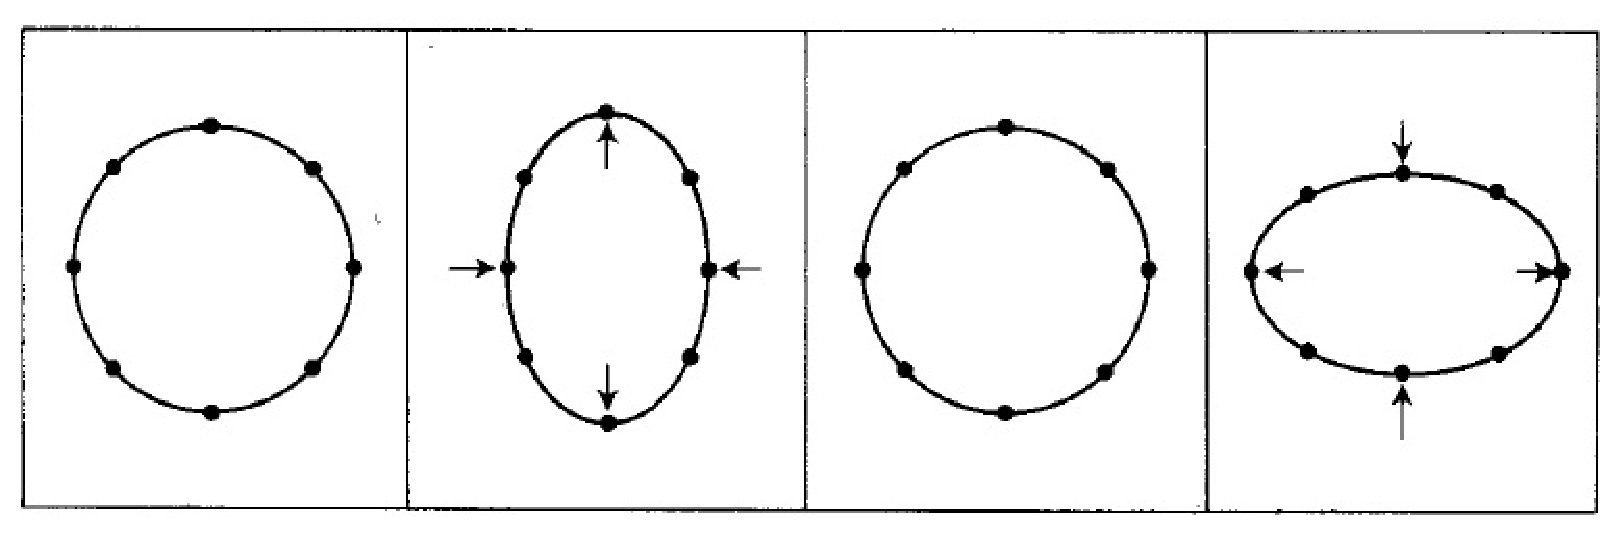
\includegraphics[width=0.5\linewidth]{figures/Introduction/pluspol.eps}
  \caption{effect of plus ($+$) polarisation}
  \label{fig:sub1}
\end{subfigure}\\
\begin{subfigure}{\textwidth}
  \centering
  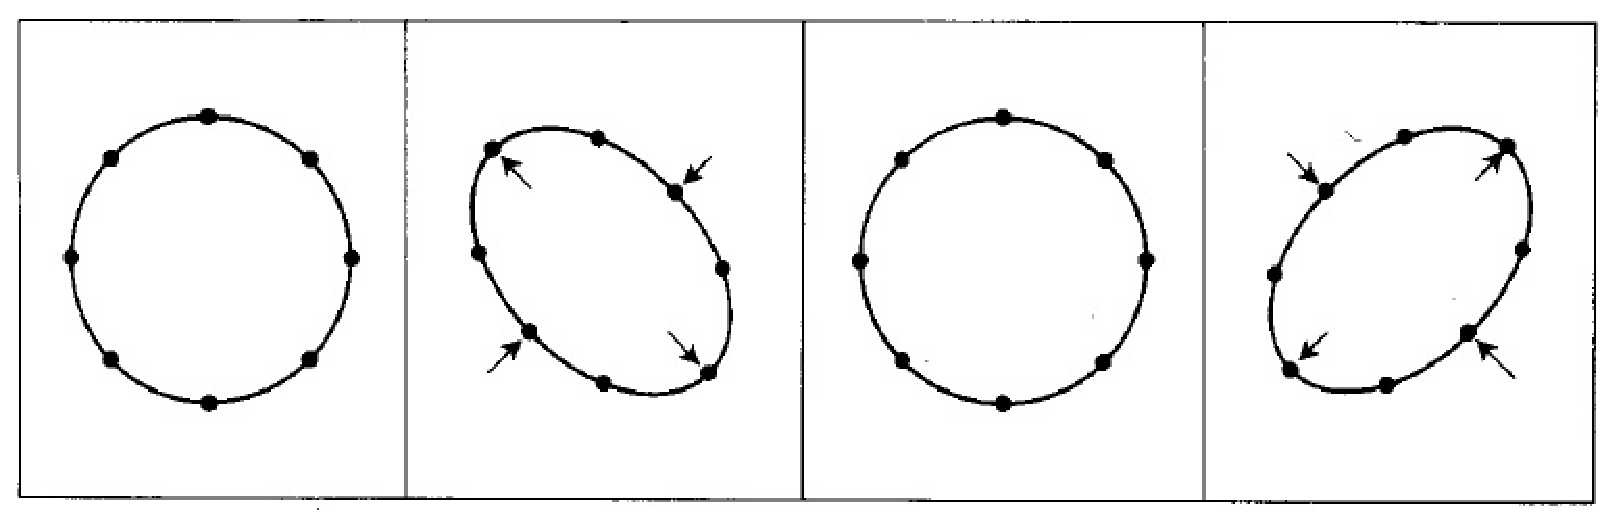
\includegraphics[width=0.5\linewidth]{figures/Introduction/crosspol.eps}
  \caption{effect of cross ($\times$) polarisation}
  \label{fig:sub2}
\end{subfigure}
\caption{Time sequence showing the effect of an oscillatory linear plane GW with (a) plus and (b) cross polarisation.}
\label{fig:Polarisation}
\end{figure}


\section{Compact Binary Mergers}

A binary system with compact objects such as black holes or neutron stars which are sufficiently close together will emit energy via the gravitational radiation. As the system evolves in frequency the radiated energy increases and the compact objects in-spiral each other. 
These are currently the most commonly detected sources of gravitational waves. 

\subsection{Modeling compact binary mergers}

A compact binary merger involves two massive objects in a close orbit, spiraling inwards due to the emission of gravitational waves, until they eventually merge. The signal from such an event can be characterized by various parameters, including the masses and spins of the two objects, the distance to the source, the inclination of the orbital plane relative to the observer, and the sky location of the source.


Different Binaries and Mathematical Formalisms:
Binary Black Holes (BBH): BBH mergers involve two black holes spiraling inwards and merging. The post-Newtonian formalism, which provides a series expansion in terms of the velocity of the objects divided by the speed of light, can be used to describe the inspiral phase. For the merger and ringdown phases, numerical relativity simulations are required, as the gravitational fields are extremely strong and the dynamics are highly nonlinear.

Binary Neutron Stars (BNS): BNS mergers involve two neutron stars. In addition to the gravitational wave emission, these events can also result in electromagnetic signals, such as gamma-ray bursts. The inspiral can be modeled using post-Newtonian formalism, but tidal effects (which are important for neutron stars) must also be taken into account. Numerical relativity simulations are required to accurately model the merger and post-merger phases, including the potential formation of a hypermassive neutron star or a black hole.

Neutron Star – Black Hole Binaries (NSBH): These binaries involve a neutron star and a black hole. The modeling of these systems is similar to BNS mergers, but with additional complexity due to the interaction of the neutron star with the black hole’s tidal field, which can lead to the disruption of the neutron star.

\subsection{Orbital mechanics and the Post Newtonian treatment}

Gravitational waves are generated by the change in the quadrupolar moment which can occur for sources that are broadly classified in four different types. \\

\begin{itemize}
\item Continuous Gravitational Waves
\item Stochastic Gravitational Wave Background
\item Supernovae
\item Primordial Gravitational Waves
\end{itemize}


\subsection{Gravitational waveforms}

Gravitational waves can be modeled by numerically solving the Einstein equations. 

A gravitational wave signal from a compact binary merger can be divided into three main parts:
Inspiral: The phase where the two objects are orbiting each other, gradually coming closer. The waveform in this phase can be approximated using post-Newtonian theory or effective-one-body formalism.

Merger: The phase where the two objects coalesce. PN approximations begin breaking down as these objects come closer. Analytical approximations are no longer valid and thus, this phase requires numerical relativity simulations for accurate modeling.

Ringdown: The phase after the merger, where the newly formed object (a black hole or a neutron star) settles into its final state, emitting gravitational waves in the process. The ringdown can be modeled using black hole perturbation theory, specifically quasi-normal modes.

Various waveform models have been proposed and developed to describe the full signal from compact binary mergers, combining analytical and numerical techniques. These include:

Phenomenological Models: These models use analytical fits to numerical relativity simulations to describe the entire waveform. Phenomenological models for gravitational waves from coalescing binary systems (such as binary black holes or neutron stars) are crucial for the detection and interpretation of gravitational wave signals. These models aim to provide accurate and computationally efficient descriptions of the signals across all phases of the coalescence: inspiral, merger, and ringdown. Below, I will delineate the construction of phenomenological waveform models, highlighting the key steps and methodologies involved.

1. Inspiraling Phase: Post-Newtonian Theory
    Post-Newtonian Expansion: The inspiral phase, where the binary components are far apart and moving slowly compared to the speed of light, is modeled using post-Newtonian (PN) theory. This involves expanding the equations of motion and gravitational waveforms in powers of $v/c$ (velocity of the bodies divided by the speed of light).

    Incorporating Spin Effects: The effects of the spins of the binary components are included using spin-orbit and spin-spin coupling terms in the post-Newtonian expansion.

    Higher-Order Corrections: The accuracy of the model is improved by including higher-order PN terms. The coefficients of these terms are calculated analytically or fitted to numerical relativity simulations.

2. Merger Phase: Numerical Relativity
    Numerical Simulations: The merger phase, where the binary components are in close proximity and moving at a significant fraction of the speed of light, requires numerical relativity simulations to accurately model. These simulations involve solving Einstein’s equations directly on a computer grid.

    Fitting to Numerical Data: The parameters of the phenomenological model are tuned to provide the best match to the numerical relativity waveforms. This process may involve fitting formulae that describe how the waveform changes with different binary parameters (such as masses and spins).

3. Ringdown Phase: Black Hole Perturbation Theory
    Quasi-Normal Modes: After the merger, the resulting single black hole undergoes a ringdown phase, emitting gravitational waves as it settles to a stable state. This phase is modeled using black hole perturbation theory, identifying the quasi-normal modes of the final black hole.

    Matching to Merger: The ringdown waveform is matched onto the end of the merger waveform, ensuring a smooth transition between the two phases.

Creating a Complete Model
    Matching Across Phases: The inspiral, merger, and ringdown phases are combined to create a complete waveform model. This requires careful matching of the waveforms at the boundaries between the phases to ensure consistency and accuracy.

    Parameterization: The complete model is parameterized in terms of the physical parameters of the binary system, such as the component masses, spins, and orbital parameters. This allows for rapid generation of waveforms for different binary configurations.

5. Validation and Calibration
    Comparison to Numerical Relativity: The phenomenological model is validated by comparing its predictions to a wide range of numerical relativity waveforms, ensuring accuracy across the parameter space.

    Calibration: The model may be calibrated to improve agreement with numerical relativity simulations, particularly in regions of the parameter space where the post-Newtonian or perturbative approximations are less accurate.

6. Application in Data Analysis
    Rapid Waveform Generation: The phenomenological model allows for the rapid generation of waveforms, which is essential for gravitational wave data analysis, including signal detection and parameter estimation.
    
    Coverage of Parameter Space: The model is designed to accurately cover the entire parameter space of binary coalescences, allowing for the analysis of a wide range of binary systems.


Effective-One-Body (EOB) Models: These models map the two-body problem onto an effective one-body problem, using results from post-Newtonian theory and numerical relativity. It was initially developed to overcome the limitations of post-Newtonian theory in the highly relativistic regime of binary mergers. 

1. Conceptual Foundation

The EOB method transforms the problem of two interacting bodies in a binary system into an equivalent problem of a single test particle moving in an effective external gravitational field. This effective field encapsulates the complex interactions between the two bodies. The transformation simplifies the problem, making it more tractable, especially in the strong-field, fast-motion regime close to merger.

2. Mapping to an Effective Problem
    Effective Metric: An effective metric is introduced to describe the gravitational field in which the test particle moves. This metric is parameterized in terms of the masses and spins of the binary components.

    Reduced Mass and Total Mass: The dynamics are described in terms of the reduced mass $\mu=\dfrac{m_1m_2}{m_1+m_2}$ and the total mass $M=m_1+m_2$, where $m_1$ and $m_2$ are the masses of the two bodies.

    Hamiltonian: An effective Hamiltonian is constructed to describe the motion of the test particle. This Hamiltonian includes not only the leading-order (Newtonian) terms but also higher-order post-Newtonian corrections and resummed terms that capture strong-field effects.

3. Resumming Post-Newtonian Terms
    Padé Approximants: The post-Newtonian series is resummed using techniques like Padé approximants to improve its convergence and extend its validity into the strong-field regime.

    Resummation of the Energy Flux: The energy flux of gravitational waves emitted by the system is also resummed to improve its behavior in the strong-field, fast-motion regime.

4. Calibration to Numerical Relativity
    Tuning Free Parameters: The EOB model includes several free parameters that cannot be determined purely analytically. These parameters are calibrated by comparing EOB predictions to fully numerical solutions of Einstein’s equations for binary systems, obtained via numerical relativity simulations.

    Improving the Model: The calibration process helps in refining the EOB model, ensuring that it accurately captures the complex dynamics of binary coalescence, especially during the merger and ringdown phases.

5. Waveform Generation
    Generating Inspirals: The EOB approach generates waveforms for the inspiral phase of the binary coalescence, capturing the increasing amplitude and frequency of the gravitational waves as the bodies spiral together.

    Extending to Merger and Ringdown: By incorporating information from numerical relativity, the EOB model is extended to accurately describe the merger of the two bodies and the ringdown of the resulting single compact object.

6. Application in Gravitational Wave Astronomy
    Parameter Estimation: EOB models are crucial for interpreting gravitational-wave signals detected by observatories like LIGO and Virgo, allowing for the extraction of physical parameters of the binary system.

    Real-time Data Analysis: Due to their efficiency in generating waveforms, EOB models are particularly useful for real-time data analysis and rapid characterization of gravitational-wave events.

7. Continuous Development and Validation
    Incorporating Spin and Precession: Efforts are ongoing to improve EOB models by incorporating effects like spin-precession and higher-order mode contributions, which are important for accurately modeling systems with spinning and misaligned components.

    Validation Across the Parameter Space: EOB models are continuously validated and updated based on comparisons with new numerical relativity simulations, ensuring their reliability across the vast parameter space of binary configurations.


Hybrid Models: These models combine post-Newtonian or EOB waveforms for the inspiral with NR waveforms for the merger and ringdown.


\section{Formation and evolution mechanisms of binary mergers}

Neutron stars (NS) and black holes (BH) with stellar masses typically emerge from the end stages of massive stars. These massive stars are usually not solitary; they often exist in pairs or even more complex groups, with many engaging in interactions with their companions, as illustrated in the works of Sana et al. (2012) and Moe and Di Stefano (2017). The dynamics of these interactions, which significantly shape the destiny and observable traits of the stars—as well as the events they catalyze, like double compact object (DCO) mergers—are not fully understood .

Gravitational wave (GW) detections offer a promising avenue for unveiling the intricate mechanisms governing the life cycles of these massive stellar entities. Yet, when such NS or BH formations are situated in regions bustling with stellar activity, the frequent stellar run-ins can modify their characteristics significantly. Under these circumstances, repeated mergers are a possibility, hinting that some GW events we observe may involve BHs that are not straightforwardly linked to the immediate outcomes of stellar or binary evolution.

One of the primary complexities in the field of GW astrophysics is the ambiguity in interpreting observational data, which can vary based on the postulated history of the merger's formation . Therefore, distinguishing the unique origins of merger events based on their observational signatures is of paramount importance.

An illustrative example is provided by the most massive GW event on record to date (GW190521), which was interpreted as a merger between two BHs with a combined mass of 150 $M_{\odot}$, with the primary BH weighing over 65 $M_{\odot}$ at a 99\% confidence level (refer to Abbott et al. 2020b,c, and see also Fishbach and Holz 2020 for a perspective that a mass over 120 $M_{\odot}$ is plausible). The formation of such a massive BH through isolated binary evolution is deemed highly improbable, as it would typically be in the range of 50 $M_{\odot}$ to 120 $M_{\odot}$ — a region expected to yield no remnant due to pair-instability supernovae (PISN), according to predictions by Bond et al. (1984) and Woosley and Heger (2006). Should GW190521 indeed include a BH mass within this predicted gap, it would strongly suggest an origin outside of isolated binary star evolution.

However, drawing broader conclusions about the evolution of massive stars from singular observations requires an understanding of how typical such instances are. As the pool of GW data grows, it allows for a more detailed understanding of the properties of local DCO mergers, such as the rates at which they occur and their mass distributions. Weaker constraints exist on their spin distributions and sky localizations, which could indicate potential host galaxies.

One particularly interesting discovery is that the bulk of the BHBH mergers observed—32 out of 44 systems—feature at least one BH exceeding 30 $M_{\odot}$ in mass. The prevalence of such massive BHs among GW findings, while anticipated due to selection biases (discussed in Sec. 1.1.2), is noteworthy since electromagnetically observed systems with BHs before the era of GW detection were estimated to be less than 20 $M_{\odot}$ (e.g., Tetarenko et al., 2016; Miller-Jones et al., 2021). The maximum mass achievable by a BH from stellar origin is understood to be metallicity-dependent, with wind mass loss rates during the massive star phase increasing with metal content, thus reducing the final mass of the BH (Vink et al. 2001; Vink and de Koter 2005). This has led to theories that the massive BHBH mergers detected through GWs may arise from low-metallicity star formation regions or potentially from previous merger events.

The potential for gravitational wave data to reveal discontinuities, such as mass gaps or cutoffs, within the compact object mass spectrum is of significant interest for its implications on core collapse and stellar explosion physics. Differing explosion models predict varying outcomes, such as a mass gap between approximately 3 - 5 $M_{\odot}$ due to the dynamics of massive stellar core collapse, with others anticipating a more uniform distribution (for instance, see Fryer et al., 2012). GW data can thus provide valuable constraints on these theoretical models.

The advancement in detector sensitivity is starting to allow examination of the BHBH population across cosmic time. The anticipated evolution of GW detector capabilities, with projects like Cosmic Explorer and Einstein Telescope (outlined by Reitze et al. 2019 and Maggiore et al. 2020), promises to map this dependency across the span of cosmic star formation history. Such insights could enhance our comprehension of the Universe's chemical evolution and its correlation with unresolved questions. This chapter will provide a comprehensive overview of these formation and evolution mechanisms.

\textbf{Formation channels}

\textbullet{Primordial Formation}

Some compact binaries are believed to form directly from the primordial gas in the early Universe. These binaries originate from density fluctuations in the early Universe, leading to the formation of closely-packed binaries.

\textbullet{Tidal Capture}

In dense stellar environments like globular clusters, stars can come close enough for tidal forces to dissipate energy and form a bound pair. Over time, through dynamical interactions and gravitational radiation, these pairs can evolve into compact binaries.

\textbf{Evolutionary Pathways}

\textbullet{Common Envelope Phase}

One of the most significant phases in the evolution of compact binary systems is the common envelope (CE) phase. This occurs when one of the stars in the binary expands, engulfing its companion. Drag forces within the envelope can cause the companion to spiral inward, leading to a closer binary system. If enough energy is released, the envelope can be ejected, leaving behind a compact binary.

\textbullet{Mass Transfer}

After the CE phase or in the absence of it, one star can transfer mass to its companion. Depending on the mass ratio and other properties, this mass transfer can be stable or unstable, leading to different outcomes:

    Roche Lobe Overflow (RLOF): When a star fills its Roche lobe, the outer layers can be transferred to its companion. This process can lead to drastic changes in the binary configuration.

    Thermal Timescale Mass Transfer: In cases where the mass-losing star is much more massive than its companion, the mass transfer can be rapid, leading to the formation of a helium core.

\textbullet{Stellar Collisions}

In dense stellar environments, direct collisions between stars can lead to the formation of compact binaries. These collisions can merge two stars or strip the outer layers of one, leaving behind a compact remnant.

\textbullet{Gravitational Radiation}

Compact binaries, especially those involving neutron stars or black holes, can emit gravitational waves. This radiation causes the binary to lose energy, leading to a decrease in the orbital separation and eventually merger.

\textbf{End Stages}

\textbullet{Supernova Explosions}

If one component of the binary undergoes a supernova explosion, it can disrupt the binary. Alternatively, if the binary remains bound, the system may evolve into a compact binary with a neutron star or a black hole.

\textbullet{Mergers}

When the separation between binary components decreases to a critical value, the binary can merge, leading to various outcomes:

    White Dwarf Mergers: Can lead to a type Ia supernova.

    Neutron Star Mergers: Result in the emission of intense gravitational waves and can form a black hole.

    Black Hole Mergers: Produce powerful gravitational waves detectable by observatories like LIGO and Virgo.







\chapter{Data analysis for gravitational-waves from compact binary mergers}

In the previous chapter we discussed modeling GW signals from compact binaries, and in this chapter we will discuss  extremely sensitive observatories to detect fractional changes in length of $\mathcal{O}(10^{-21})$ and sophisticated data analysis techniques to find signals buried under large volumes of noisy data.  We will first give an overview of the ground based laser interferometers, along with an overview of the broad sources of noise in them. We will briefly talk about the existing observatories and those proposed for the future. Next, we will discuss the key components of data analysis techniques used for searching GW signals.    

%The indirect detection of gravitational waves (GWs) through the Hulse-Taylor binary pulsar represents a pivotal moment in astrophysics. Discovered in 1974 by Russell Hulse and Joseph Taylor, this binary system consists of a pulsar orbiting another neutron star. Over time, precise measurements of the pulsar's orbit exhibited a gradual decay in its orbital period. This decay matched predictions from Einstein's theory of General Relativity, which suggested that the system should be losing energy through the emission of gravitational waves. The energy loss rate, inferred from the changing orbital period, was found to be in excellent agreement with the theoretical predictions for gravitational wave emission. Although this was an indirect observation, it provided the first compelling evidence of the existence of gravitational waves and earned Hulse and Taylor the Nobel Prize in Physics in 1993. Their discovery not only confirmed a major prediction of General Relativity but also paved the way for future direct detections of gravitational waves. 


\section{Ground-based interferometers}
The earliest GW detectors were constructed by Joseph Weber (in 1960s) called as the \textit{Weber bar}, consisting of aluminum bar of 2 meters in length and a meter in diameter \cite{Weber:1960zz}. The Weber bars' principle idea for detection was using vibration at the resonance frequency of $\sim 1.6$ KHz. Resonant bars were not sensitive to detect any GWs and could only pick up signals with a strain around $\sim 10^{-16}$, which is significantly higher than the zero-order quadrupole strain of $h \sim 10^{-21}$ as calculated earlier. To put it in perspective, this level of sensitivity would only allow for the detection of a Binary Black Hole (BBH) merger occurring within a distance of about 1 kiloparsec (within our Milky Way), an event highly improbable given current estimates of such occurrences and conventional models of astrophysical binary populations \cite{Nitz:2021zwj,LIGOScientific:2021djp,Olsen:2022pin, Belczynski:2001uc,vandenHeuvel:2017pwp, Marchant:2016wow, Fragione:2018vty, Rodriguez:2017pec,Sedda:2020wzl}.

GWs cause matter to stretch in one direction while simultaneously squeezing the perpendicular direction. Leveraging this fundamental principle for detection, in the late 1960s a parallel effort kick started to make prototype interferometeric gravitational wave detectors. Over subsequent decades, extensive collaborative efforts across multiple fields – including instrumentation, engineering, and applied physics – were dedicated to enhancing the sensitivity of these massive interferometers. This combined effort made it possible to achieve the necessary precision to detect gravitational waves. In the next subsection, we briefly discuss the principle mechanism of interferometers required for detecting these waves. 


\subsection{LASER interferometers}
Today's ground-based GW observatories employ an evolved concept of a Michelson interferometer with the addition of a Fabry-Pe\'rot cavity. Currently there are five operational gravitational wave observatories: the Advanced Laser Interferometer Gravitational-Wave Observatory (LIGO) detectors in Hanford, (Washington), and Livingston, (Louisiana), in the United States \cite{LIGOScientific:2014pky}; Virgo, located near Pisa, Italy \cite{VIRGOdetector}; KAGRA, in Japan \cite{KAGRA:2018plz} and the GEO 600 in Sarstedt, Germany \cite{Dooley:2015fpa}. These detectors are part of a growing global network that collaborates to triangulate the source of gravitational waves and improve the sensitivity of detections. 


%The Advanced LIGO observatories in Hanford and Livingston are identical in their L-shaped design, with each arm being 4 kilometers long. The arms are kept in a near-perfect vacuum to minimize disturbances, and mirrors at the ends of each arm are suspended to isolate them from external vibrations. Virgo is a gravitational wave detector that features a 3-kilometer-long L-shaped interferometer. While slightly shorter than the LIGO arms, Virgo is crucial because of its longer duty cycle. KAGRA is unique among the ground based detectors as it is located underground in the Kamioka mine, which helps to shield it from seismic noise and provides a stable thermal environment. KAGRA uses a 3-kilometer-long L-shaped interferometer like Virgo and is designed to operate at cryogenic temperatures to reduce thermal noise. Despite its smaller size, GEO 600 compensates with advanced technologies, particularly in precision optics and LASER stabilization, making it a valuable test-bed for innovative techniques in gravitational wave detection. These advancements have often been instrumental in enhancing the sensitivity of the larger interferometers. 


\begin{figure}
    \centering
    \includegraphics[width=\textwidth]{figures/basic_data_analysis/GW-observatories.png}
    \caption{Gravitational wave observatories around the World. LIGO Livingston and Hanford, Virgo and KAGRA contributing to scientific observing runs. The Advanced LIGO observatories in Hanford and Livingston are identical in their L-shaped design, with each arm being 4 kilometers long. Virgo is a gravitational wave detector that features a 3-kilometer-long L-shaped interferometer. KAGRA is unique 3-kilometer-long L-shaped interferometer, as it is located underground in the Kamioka mine. GEO600 is a nearly L-shaped interferometer with arm lengths of 600m, and serves as a key site to test technologies for the bigger observatories. Photo credits: LIGO, Joe Giaime, GEO600 and KAGRA.}
    \label{fig:GW-observatories}
\end{figure}


Michelson interferometer was successfully employed during the famed Michelson-Morley experiment in 1887 designed to verify the presence of an aether wind \cite{Michelson:1887zz}. In a simple Michelson interferometer (shown in Fig. \ref{fig:Michelson-interferometer}), a single beam of monochromatic light (usually a LASER) is directed towards a beam splitter. This mirror splits the beam into two separate but perpendicular paths: one continues straight while the other is reflected at a 90-degree angle. In normal conditions, without gravitational waves, these beams travel back and forth over the same distance and converge at the photodetector, resulting in destructive interference, effectively cancelling each other out. During the passing of an astrophysical GW signal will cause one arm of the interferometer to extend and the other to shrink (Fig. \ref{fig:Polarisation}). This alters the optical paths of the beams, leading to a time delay upon their return to the photodetector. Instead of cancelling out, they create a pattern of constructive interference. A photodetector is positioned at the output port to receive the beam and generate the readout. 
%This unique interference pattern serves as a detectable signature, characteristic of the astrophysical source of the gravitational wave. 

The interferometers measure ``strain", which is a dimensionless measure of the fractional change in length that one of the interferometer's arms experiences relative to the other. The minimum change in the interferometer's arm length is limited by the wavelength of the laser $\lambda_{\text{laser}} \sim \Delta L$. To the first order, the fractional change in the interferometer’s arm length is given by
\begin{align}
    \dfrac{\Delta L}{L} \simeq \dfrac{\lambda_{\text{laser}}}{L} \simeq 10^{-9}, 
    \label{Eq:rough-strain-sensitivity}
\end{align}
using arm lengths $\mathcal{O}$(1 km) and lasers with wavelength $10^{-6}$m. In comparison,  typical GW strain is $\sim 10^{-21}$ (using Eqs. (\ref{Eq:ring-eqn}) and (\ref{Eq:toymodel-plus})), several orders of magnitude smaller than what could be detected by a simple Michelson interferometer.  
%We can write the phase difference accumulated with a LASER of wavelength $\lambda_l \sim 1 \mu m$, as \cite{Maggiore:2008aaa} 
%begin{align}
%    \Delta \Phi = \dfrac{4\pi}{\lambda_L}h_+L \sim 10^{-12}.  
%\end{align}

To improve the inteferometer's ability to reach required sensitivity, additional components are employed that increase the effective path length and power of the laser. The light from beam splitter is trapped inside a \textit{Fabry-P\'erot} \cite{Maggiore:2008aaa} cavity (two parallel, highly reflective mirrors), allowing it to bounce back and forth -- increasing the effective distance travelled by each laser from $4$km to $\sim 1000$km. Increasing the power of the laser also improves the performance of the interferometer -- more number of photons leads to sharper fringes at the photodetector. To achieve this, a \textit{power recycling mirror} is used to reflect the laser light that has already passed through the instrument, back into the interferometer, effectively `recycling' it \cite{Meers:1988wp}. This continuous cycling of laser power, coupled with the constant influx of light from the laser source, significantly enhances laser light's power inside the interferometer without the necessity of initially producing an extremely powerful laser beam. A similar technique is used to recycle the power of the light before it reaches to the photodetector, called \textit{signal recycling} \cite{Buonanno:2001cj}. 

These enhancements allow the interferometers to reach the sensitivity of $h \sim 10^{-21}$. At such small length deviations, numerous factors impact the movement of the test masses and the detectable output signal, acting as noise that constrains the detectors' sensitivity. These noise sources are largely well-characterized and can be effectively modeled, as discussed next. 

\begin{figure}
    \centering
    \includegraphics[width=0.5\textwidth]{figures/basic_data_analysis/Michelson-interferometer.png}
    \caption{A simplified design of a LASER interferometer: The left panel presents a basic diagram of a LASER interferometer with its arms aligned along the $x$ and $y$ axes. A beam splitter divides the incoming laser light, directing it into two arms, each housing a Fabry-Pérot cavity. These beams are then merged back together and captured at the output. Image credits: \cite{Kondrashov:2008zr}}
    \label{fig:Michelson-interferometer}
\end{figure}

\subsection{Noise sources}
Achieving the extraordinary sensitivity means that these detectors have to deal with a plethora of noise sources that can mask or mimic gravitational-wave signals.  To keep track of the detector's internal condition and its surrounding physical environment, a variety of additional sensors are employed, gathering data through auxiliary channels. Below is an expanded look at the main types of noise that affect ground based gravitational wave observatories:

Quantum noise in gravitational wave detectors arises from the Heisenberg uncertainty principle, which limits the precision with which pairs of physical properties, like position and momentum, can be known. A technique called \textit{squeezing} is used to swap the uncertainties in the measurement of amplitude or phase of the noise, which is related by the Heisenberg uncertainity principle \cite{Oelker2016}. 
\begin{itemize}
    \item Shot Noise: This is a form of quantum noise that arises because light consists of discrete particles (photons). When measuring the interference pattern in an interferometer, the discrete arrival of photons causes statistical fluctuations in the detected light intensity. At high laser power, shot noise predominates and limits the high-frequency sensitivity of the detectors \cite{Tse2019}.
    \item Radiation Pressure Noise: At lower frequencies, the variability is dominated by radiation pressure noise. This is the fluctuation in force exerted by photons as they bounce off the mirrors. It introduces a quantum limit to the low-frequency sensitivity due to the momentum transfer of the light \cite{Kondrashov:2008zr}.
\end{itemize}

The inherent Brownian motion of the atoms in any macroscopic object at a given temperature generates thermal noise. This effect impacts both the mirrors and the suspension system \cite{Levin:1997kv}:
\begin{itemize}
    \item Suspension Thermal Noise: The motion of the suspension fibers can introduce noise due to thermal vibrations. Advanced detectors use materials such as fused silica with very low mechanical losses to suspend the mirrors, minimizing this source of noise \cite{Aston:2012ona}.
    \item Mirror Thermal Noise: The mirrors themselves are also sources of thermal noise. Brownian motion within the reflective coating and the substrate material of the mirrors can lead to fluctuations in the reflected light phase \cite{Braginsky:2003yhs}. Lowering temperatures (as with KAGRA) can reduce such noise \cite{Steinlechner:2018crl}. Additionally, the Brownian noise of the mirror coatings also has a non-negligible impact, which can be reduced by using improved AlGaAs coatings (as planned for future observatories) \cite{Cole:2023sak}.  
\end{itemize}

Seismic noise is the result of ground vibrations transmitted through the Earth, originating from natural and anthropogenic sources: 
\begin{itemize}
    \item Ground Vibrations: These are the primary source of noise below a few tens of hertz. They can be caused by earthquakes, ocean waves, or even nearby human activity such as traffic or industrial work. Advanced isolation systems are used to minimize this noise, including active seismic isolation, which uses sensors to detect ground motion and actuators to counteract it, and passive isolation, such as layers of springs and masses that absorb vibrations \cite{Aston:2012ona,Daw:2004qd}.
\end{itemize}

Gravity gradient noise, also known as Newtonian noise, is due to fluctuations in the local gravitational field \cite{Harms:2015zma,Saulson:1984yg}:
\begin{itemize}
    \item  Environmental Factors: These can be caused by atmospheric pressure changes, density changes in the Earth, or even human activity, all of which can create varying gravitational forces on the detector components. This type of noise is particularly challenging to mitigate because it cannot be shielded against in the same way as electromagnetic noise. Efforts to subtract it involve modeling the environmental effects and removing their signature from the data \cite{Harms:2020uyc}.
\end{itemize}

Instrumental noise arising from the detector components:
\begin{itemize}
    \item  Electronic Noise: In the photodetectors and other electronic systems, inherent noise can be introduced. This is typically white noise that can be well-characterized and filtered \cite{Kondrashov:2008zr}.
    \item Calibration Errors: Uncertainty in the detector's response to gravitational waves can also introduce noise into the measurement. Regular calibration is necessary to minimize this noise \cite{Sun:2020wke}.
\end{itemize}

Despite efforts to correlate noise with auxiliary channels, numerous types of short noise artefacts \textit{glitches} remain persistent in the data which reduce our confidence for detection by mimicking GW signals. Certain types of transient noises, namely Blips, Tomte, and Koi-Fish, have been observed to happen at a frequency of about once per hour \cite{Cabero:2019orq}. To date, these glitches have not been definitively linked to any environmental or instrumental causes \cite{Cabero:2019orq}. Eradication of glitches require additional vetoeing technqiues while searching for GW signals, which will be discussed later in this chapter.  

\begin{figure*}
    \centering
    \includegraphics[width=\textwidth]{figures/basic_data_analysis/O3_noise_budget.PNG}
    \caption{O3 noise budget. Only few noise sources are shown for a simplified picture. Image credits: \cite{aLIGO:2020wna}}
    \label{fig:O3_noise_budget}
\end{figure*}



\subsubsection{Upcoming and future observatories}

There are two upgrades planned for the current Advanced LIGO observatories for the post-O5 timeline -- LIGO A+ and LIGO $\text{A}^{\#}$. LIGO A+ is expected to be $2\times$ more sensitive than Advanced LIGO and would involve improvements such as better seismic noise isolation and test mass suspensions \cite{KAGRA:2013rdx}. Further factor of two improvement is expected with LIGO $\text{A}^{\#}$ with reduction in quantum noise and coating thermal noise \cite{Asharp}.

%.  LIGO $\text{A}^{\#}$, is the upgrade further aimed towards boosting sensitivity the following O5 observation run, slated for 2029. This upgrade is designed to fill the observational gap and maintain continuity in gravitational wave research until the third-generation facilities, such as the Cosmic Explorer and Einstein Telescope, become operational.

Third-generation (3G) gravitational wave detectors, such as the Cosmic Explorer and the Einstein Telescope are planned to become operational by mid 2030s \cite{Gupta:2023lga,Punturo:2010zz}. The Cosmic Explorer, with its proposed arm lengths of up to 40 kilometers, aims to increase up to an order of magnitude in sensitivity and observational range over current detectors \cite{Evans:2021gyd}. The Einstein Telescope, planned to be an underground facility in Europe with a triangular configuration of 10-kilometer arms, seeks to reduce seismic noise and enhance detection capabilities \cite{Hild:2010id}. The location of both the 3G observatories is not yet finalized, but is strongly preferred to be in the USA for CE and in Europe for ET. 

Ground-based interferometers are limited by seismic noise, especially at frequencies below one Hertz. To circumvent this, efforts have shifted to space-based interferometers, such as the Laser Interferometer Space Antenna (LISA) \cite{LISA:2017pwj}. A collaborative project between the European Space Agency and NASA, LISA is set for a 2030s launch \cite{LISA-intro, LISA:2017pwj, eLISA:2013xep} after the success of the test mission LISA Pathfinder \cite{Armano:2016bkm,McNamara:2008zz}. LISA will consist of three spacecraft forming a vast triangle, each side stretching 2.5 million kilometers, in space. LISA's science case is rooted in its potential to open new windows for new source like Extreme Mass Ratio Inspirals (EMRIs), Intermediate Mass BBHs (IMBBH) mergers, galactic binary inspirals and cosmological stochastic background \cite{eLISA:2013xep}. The noise curves for various GW observatories mentioned above are shown in the Fig. (\ref{fig:Gw-plotter}).

\begin{figure}
    \centering
    \includegraphics[width=\textwidth]{figures/basic_data_analysis/Gw-plotter.png}
    \caption{Sensitivity curves and expected strains: Bold lines show predicted senstivity curves for various GW detectors, including ground based Advanced LIGO observatory, space based LISA and International Pulsar Timing Arrays. Senstivity curves for some proposed observatories for the future -- A+, Cosmic Explore, LISA are also shown. The shaded regions show characteristic strain for various sources as labelled. Source: \href{http://gwplotter.com/}{GW-plotter}.}
    \label{fig:Gw-plotter}
\end{figure}

\subsubsection{Signal observed at a ground based detector}
In Eqs. (\ref{Eq:toymodel-plus}) and (\ref{Eq:toymodel-cross}), we performed the transformation of gravitational radiation from the source to the radiation frame. An additional projection of the signal is necessary due to the detector's varying sensitivity across different sky points. This involves transforming the signal to the detector frame using three Euler angles, determined by the sky location of the source $(\alpha,\delta)$ known as the declination and right ascension and the polarization angle $\psi$ which signifies the rotation of the wavefront along the line of sight. The signal observed at the detector is then written in terms of the linear combination of the two polarizations
\begin{align}
    h(t) = F_+h_+ + F_{\times}h_{\times},
    \label{Eq:}
\end{align}
where the co-efficients are the \textit{antenna pattern functions} of the detector as shown in the Fig. \ref{fig:antenna-pattern}, and are given by \cite{Schutz:2011tw}
\begin{align}
    F_{+}(\alpha,\delta,\psi) = -\dfrac{1}{2}(1+\cos^2\alpha)\cos 2\delta\cos 2\psi -\cos\alpha\sin 2\delta\sin 2\psi, \\
    F_{\times}(\alpha,\delta,\psi) = \dfrac{1}{2}(1+\cos^2\alpha)\cos 2\delta\sin 2\psi -\cos\alpha\sin 2\delta\cos 2\psi.
    \label{Eq:det-frame-signal}
\end{align}


\begin{figure}
    \centering
    \includegraphics[width=\textwidth]{figures/basic_data_analysis/antenna-pattern.png}
    \caption{Angular distibution of the antenna pattern functions of an observatory in the $x-y$ plane.}
    \label{fig:antenna-pattern}
\end{figure}


\subsection{Basics of Fourier domain analysis}

Fourier domain analysis is a mathematical technique widely used in the field of data analysis to extract signal information from noisy data. Gravitational-wave signals are often buried in noise, making it difficult to detect them in the time domain. However, by transforming the data into the frequency domain using Fourier analysis, it becomes easier to identify and analyze these signals.


Suppose we have a function of time $x(t)$. Let us denote the Fourier transform of $x(t)$ by $\tilde{x}(f)$, which is given by
    \begin{align}
        \tilde{x}(f) = \int_{-\infty}^{\infty} e^{-2\pi i ft} x(t) dt,
    \end{align}
    similarly, the inverse Fourier transform is given by
    \begin{align}
        x(t) = \int_{-\infty}^{\infty} e^{2\pi i f t} \tilde{x}(f) df.
    \end{align}

\subsubsection{Discrete Fourier Transform}
Continuous signals $x(t)$ are analyzed by sampling at discrete intervals of $\Delta t$ to create a finite set of data points $x[t_i]$. If this signal is band-limited to a maximum frequency $f_{max}$, then the sampling interval $\Delta t$ is determined by adhering to the \textit{Nyquist-Shannon} sampling theorem \cite{Nyquist-shannon} -- the sampling frequency $f_s \equiv 1/\Delta t > 2f_{max}$. We can then write the Discrete Fourier Transform (DFT) of $x[t]$ assuming $N$ samples, as
\begin{align}
    \tilde{x}[f_k] = \Delta t \sum_{j=0}^{N-1} x[t_j] e^{-2\pi i j k/N},
\end{align}
and similarly the Inverse DFT as
\begin{align}
    x[t_k] = \Delta f \sum_{j=0}^{N-1} \tilde{x}[f_j] e^{2\pi i j k/N},
\end{align}
where $\Delta f \Delta t = 1/N$.

The DFT assumes that the input sequence is one period of a periodically repeating signal. This implies that the DFT treats the data as if it were part of a periodic sequence. The direct computation of DFT requires $O(N^2)$ operations, which can be expensive for large number of samples. 

The Fast Fourier Transform (FFT) most famously in the form of the Cooley-Tukey algorithm to reduce the computational complexity of the DFT \cite{Cooley-Tukey}.  The FFT algorithm exploits the periodicity and symmetry of the complex exponential function to reduce redundancy in computations, applying the algorithm recursively to increasingly smaller DFTs, and then efficiently combining these results which reduces the complexity to $O(N\log N)$.


\subsection{Modeling and measuring the noise}
The noise time series in a detector like LIGO is a complex superposition of various stochastic processes. We represent this time series $n(t)$ as a vector $\textbf{n}$ (or random process), where each of the discrete samples $n_i = n(t_i)$ is described as random variable with values according a probability distribution $p_i = p(n_i)$. The complete noise vector is then associated to to a joint probability distribution $p(\textbf{n})$. 

Features of any probability distribution can be captured by measuring moments. The first two moments of a stochastic process are often of particular interest -- mean $\mu = \langle \textbf{n}\rangle$ and covariance $C_{ij} = \langle(n_i-\mu)(\mu-n_j)\rangle$, where $\langle\rangle$ is defined as the expectation value of a random variable over time. The ensemble average is equivalent to a long time average. We can estimate these two quantities from the data with $N$ data samples uniformly sampled with sampling interval $\Delta T$
\begin{align}
    \mu = \dfrac{1}{N}\sum_{i=1}^{N}n_{i}.
    \label{eq:mean-noise-series}
\end{align}
And, the covariance matrix can be estimated using
\begin{align}
    C_{ij} = \langle (n_{i} - \mu)(\mu - n_j) \rangle.
    \label{eq:covariance-noise-series}
\end{align}
The covariance matrix allows us to estimate the \textit{power spectrum} which is essential in characterizing the noise. The power spectrum can be shown to be the expectation value of $n^2$ over a large duration of time interval $T$,
\begin{align} 
   \langle n^2 \rangle &= \lim_{n\to\infty} \dfrac{1}{T} \int_{-\infty}^{\infty} |n_T(f)|^2 df,\\
   & = \int_0^{\infty} S_n(f) df,
\end{align}
where $n_T(t) = n(t)w_T(t)$ is a windowed signal within $-T/2 < t < T/2$ and $S_n(f)$ is the \textit{power spectral density} of the process $n(t)$ (we refer the reader to \cite{Allen:2005fk} for a detailed derivation). Now, we model the noise by assuming zero mean and by using three properties that will help characterize the noise better, these properties are: 

\subsubsection{Stationary}
A stochastic process is known as wide-sense \textit{stationary} process where the statistical properties are invariant with time. Specifically, for a process to be considered wide-sense stationary, it must satisfy two main conditions: 1. the mean of the process is constant over time and 2. the covariance function $C_{ij}$ depends only on the time difference (lag) and not on the specific time. Using the stationarity conditions, the covariance matrix can be written as
\begin{align}
    C(n(t), n(t+\tau)) = \langle n(t)n(t+\tau) \rangle = R_n(\tau),
\end{align}
for all $t$ and $\tau$, where the \textit{autocorrelation function} $R_n(\tau)$ is the correlation between a signal with a delayed copy of itself.

Assuming the noise process to be wide-sense stationary, the power spectral density can be related by the \textit{autocorrelation} function $R_n(\tau)$ using the Wiener-Khinchin theorem as
\begin{align}
    S_n(f) := \int_{-\infty}^{\infty} R_n(\tau)e^{- i2\pi f\tau} d\tau.
    \label{Eq:Weiner-Khinchin}
\end{align}

Another useful property of power spectral density in the Fourier domain is that the expectation value of two frequency components $\tilde{x}(f)$ and  $\tilde{x}(f')$ is proportional to the Dirac delta function $\delta(f-f')$
\begin{align}
    \langle \tilde{n}^*(f') \tilde{n}(f) \rangle = \dfrac{1}{2}S_n(f)\delta(f-f').
    \label{Eq:PSD-prop-fourier}
\end{align}

%where $\tau$ is the lag, or the time difference between the signal and its delayed version. For noise process with zero mean, it can be shown from Eq. () that the covariance matrix is the same as the autocorrelation function
%\begin{align}
%    C(\tau) = R_n(\tau) \hspace{1cm} \text{for} \hspace{1cm} (\langle \textbf{n} \rangle = 0).
%\end{align}

\subsubsection{Colored}
We first consider a simple case of white noise, which is characterized by a constant power spectral density across all frequencies within a given bandwidth. This means that every frequency component has the same power
\begin{align}
    S_n(f) = S_0.
\end{align}
In case of white noise, the covariance matrix is a constant $C_{ij} = S_0/\Delta t$, where $\Delta t$ is the sampling interval.

Colored noise has a PSD that changes depending on the frequency. This variation can take different forms, such as $S_n(f) \propto 1/f$ known as pink noise. Using $S_n(f)$ as the PSD for a stationary colored noise, the covariance matrix is diagonalized and can be written as
\begin{align}
    C_{ij} = S_n(f_i)\delta_{ij}
    \label{Eq:Colored-noise-PSD}
\end{align}
 
\subsubsection{Gaussian}

This property allows us to write the joint probability distribution of noise time-series $p(\textbf{n})$ with $N$ samples, following a multi-variate normal distribution using the mean and covariance matrix described above 
\begin{align}
    p(\textbf{n}) = \dfrac{1}{(2\pi)^{N/2}\sqrt{\text{det}(\textbf{C})}}\text{exp}\Bigg[-\dfrac{1}{2} \sum_{ij}n_{i}C_{ij}^{-1}n_j  \Bigg],
    \label{Eq:joint-pdf-noise}
\end{align}
where $C_{ij}^{-1}$ represents the inverse and $\det(\textbf{C})$ the determinant of the covariance matrix. We define the matrix $G_{ij}$ as the inverse of the covariance matrix, which is given by $G_{ij} = 1/S_n(f)$. Using Eq. (\ref{Eq:joint-pdf-noise}), we can simplify the exponent part of the joint probability distribution 
\begin{align}
    p(\textbf{n}) & \propto \exp \Bigg[ - \dfrac{1}{2} \sum_{ij} \dfrac{n_i \delta_{ij} n_j}{S(f)} \Delta t \Bigg]\\
    &  \propto  \exp \Bigg[ - \dfrac{1}{2} \int_{0}^{T} \dfrac{n(t)^2}{S(f)} dt \Bigg] \\
    &  \propto  \exp \Bigg[ - \dfrac{1}{2} 4\int_{0}^{\infty} \dfrac{|\tilde{n}(f)|^2}{S(f)} df \Bigg],
\end{align}
where we have used that $n(t)$ is real-valued implying $\tilde{n}(-f) = \tilde{n}^*(f)$.

Defining a noise-weighted inner product between two time series $x(t)$ and $y(t)$ as,
\begin{align}
    (x|y) := 4 \Re \int_{0}^{\infty} \dfrac{\tilde{x}(f)\tilde{y}^*(f)}{S_n(f)} df,
    \label{Eq:inner-product}
\end{align}
we can write the probability density for a stationary Gaussian colored noise process $n(t)$ concisely as,
\begin{align}
    p(\textbf{n}) \propto e^{-(\textbf{n}|\textbf{n})/2}.
    \label{Eq:noise-probability}
\end{align}

\section{Optimal method to extract signal out of noise: Matched-filtering}

Matched-filtering technique is at the heart of modeled approaches for detecting compact binary coalescence (CBC) signals. This technique is performed in the Fourier domain, which estimates the probability of a stretch of data containing an anticipated signal $\tilde{h}(f)$ within Gaussian noise. The statistic used in matched-filtering is essentially a correlation involving the Fourier-transformed data $\tilde{s}(f)$ and a template $\tilde{h}(f)$ weighted by the noise power spectral density (PSD) $S_n(f)$. The complex matched-filter statistics is defined as 
\begin{align}
    \label{Eq:complex_matched_filter}
    \braket{s|h} = 4\int_{0}^{\infty} \dfrac{\tilde{s}(f)\tilde{h}^*(f)}{S_n(f)},
\end{align}
and the real component of this complex matched-filter is same as the inner product defined in Eq. (\ref{Eq:inner-product})
\begin{align}
    (s|h) = \Re [\innerproduct{s}{h}].
\end{align}
We define the output of the matched-filter as the signal-to-noise ratio (SNR)
\begin{align}
    \label{Eq:SNR_def}
    \rho^2 \equiv \dfrac{(\Real[\braket{s|h}])^2}{\braket{h|h}} = \dfrac{(s|h)^2}{(h|h)}.
\end{align}

We can show the matched-filter is an optimal detection statistic which maximizes the SNR, by invoking the Neyman-Pearson criterion \cite{Wainstein1963}. This criterion maximizes the probability of correctly rejecting a false null hypothesis (true positive) at a given probability of incorrectly rejecting a true null hypothesis (false positive). 

We assume the strain data $s(t)$ contains noise process $n(t)$ with or without a possible GW signal with known form $h(t)$, to construct two hypotheses:
\begin{align}
    \text{Null Hypothesis} \hspace{1em} \mathcal{H}_0 :  & s(t) = n(t), \\
    \text{Alternate Hypothesis} \hspace{1em} \mathcal{H}_1 : & s(t) = h(t) + n(t).
\end{align}
Assuming Gaussian noise, we can then compute the probability density for each hypothesis as (from Eq. (\ref{Eq:noise-probability}))
\begin{align}
    p(s|\mathcal{H}_0) & \propto e^{-(s|s)/2},\\
    p(s|\mathcal{H}_1) & \propto e^{-(s-h|s-h)/2}.
\end{align}
Then using Bayes's theorem we can write the likelihood ratio as
\begin{align}
    \Lambda(\mathcal{H}_1|s) = \dfrac{p(s|\mathcal{H}_1)}{p(s|\mathcal{H}_0)},
\end{align}
and substituting the probabilities for the two hypothesis to get the log-likelihood ratio as
\begin{align}
    \log\Lambda(\mathcal{H}_1|s) = (s|h) - \dfrac{(h|h)}{2}.
\end{align}
Now, suppose if the signal as an unknown amplitude $h(t) = Ah_0(t)$, then we can maximize the log-likelihood ratio over this parameter to get
\begin{align}
    \max_{A} [\log\Lambda(\mathcal{H}_1|s)] = \dfrac{(s|h_0)^2}{(h_0|h_0)} = \dfrac{\rho^2}{2}
\end{align}
which is related to the matched filter SNR from Eq. (\ref{Eq:SNR_def}).

%which is a monotonically increasing function of the data $s(t)$ only via the term $(s|h)$.  

%It can be shown that matched-filter provides the optimal statistical measure, by maximizing the signal-to-noise ratio (SNR) \cite{Maggiore:2008aaa,Creighton-book}
%The signal-to-noise (SNR) ratio $\rho$ which is the matched-filter output maximised over an overall amplitude,   

%This technique scans through data from interferometers to identify patterns that match the anticipated GW signal waveform $\tilde{h}(f)$. This technique is performed in the frequency domain to detect the anticipated GW signal, denoted as $\tilde{h}(f)$, commonly referred as the \textit{template}. 

%Knowing the statistical characteristics of the noise and the precise nature of the signal enables the creation of an optimal detection statistic, which quantifies the likelihood that the data includes the expected signal.




%and the likelihood depends on the data only via the inner products $(s|h)$ and $(h|h)$. 
%Thus the noise-weighted inner product, called as \textit{matched-filtering} is the optimal detection statistic.

%The mathematical expression for the complex matched-filter statistic is:


\subsection{Unknown signal parameters}\label{sec:MF-maximization}
The previous section dealt with calculating the optimal statistic for known GW signals or those differing only in amplitude. In practice, the signal parameters are unknown a priori,  necessitating the maximization of SNR across the entire parameter space of astrophysical signals. We simplify the signal parameter space by assuming quasi-circular systems with only the dominant ($2,2$) mode of the GW emission which are described by 15 distinct parameters. We categorize the parameters into two groups: (1) intrinsic parameters $\vec{\zeta}$ -- the component masses $(m_1, m_2)$ and three-dimensional spin vectors $(\vec{\chi_1}, \vec{\chi_2})$, and (2) extrinsic parameters $\gamma$, that are defined from the perspective of the observer, these are: the standard spherical coordinates -- distance and inclination of the source, the reference orbital phase at coalescence $(d_L, \iota, \Phi_c)$, position in the sky $(\alpha, \delta)$, polarization $\psi$, and the coalescence time $t_c$.

Searching over a broad range of sources over the complete 15-dimensional parameter space is computationally challenging. A simplified procedure is to invoke analytical approximations that help reduce the problem to fewer variables. To demonstrate this procedure, we begin with the signal seen by the detector in Fourier domain is given by, 
\begin{align}
    \tilde{h}(f) &= F_{+}(\alpha,\delta,\psi)\tilde{h}_{+}(\vec{\zeta}, d_L,\iota;f) + F_{\times}(\alpha,\delta,\psi)\tilde{h}_{\times}(\vec{\zeta}, d_L,\iota;f).
\end{align}
We can simplify the signal by combining $F_+$ and $F_{\times}$ and using normalized templates 
\begin{align}
    \hat{h} = \dfrac{\tilde{h}}{\innerproduct{\tilde{h}}{\tilde{h}}^{1/2}}.
\end{align}
The above equation allows us to freely scale the amplitude of the templates. Writing the templates and antenna pattern functions by omitting the parameters for the sake of brevity, we get
\begin{align}
    \tilde{h} &= A(u\hat{h}_+ + \hat{h}_{\times}), 
    \label{Eq:detector-signal-fourier-domain}
\end{align}
where
\begin{align}
    u = \dfrac{F_{+}}{F_{\times}}\sqrt{\dfrac{\innerproduct{\hat{h}_{+}}{\hat{h}_{+}}}{\innerproduct{\hat{h}_{\times}}{\hat{h}_{\times}}}},
\end{align}
and
\begin{align}
    A = F_{\times}\sqrt{\innerproduct{\hat{h}_{\times}}{\hat{h}_{\times}}}.
\end{align}
Inserting the Eq. (\ref{Eq:detector-signal-fourier-domain}) into (\ref{Eq:SNR_def}), the amplitude term gets cancelled. Maximising SNR over $u$ results into \cite{Harry:2017weg}
\begin{align}
    \max_{u}(\rho^2) = \dfrac{(s|\hat{h}_{+})^2 +
                            (s|\hat{h}_{\times})^2 
                            - 2(s|\hat{h}_{+})(s|\hat{h}_{\times})(\hat{h}_+|\hat{h}_{\times})}{\Big(1-(\hat{h}_+|\hat{h}_{\times})^2\Big)}.
    \label{Eq:Generic-SNR-maximization}
\end{align}

Eq. (\ref{Eq:Generic-SNR-maximization}) indicates the SNR maximization problem reduces to only the intrinsic parameters ($\vec{\zeta}, \iota, \Phi_c$ and $t_c$). Assuming the component spins to be aligned with the orbital angular momentum and by searching only using the dominant gravitational-wave mode, we get  
\begin{align}
    \hat{h}_{+} \propto i\hat{h}_{\times},
    \label{Eq:polarization-symmetery}
\end{align}
which implies $\innerproduct{\hat{h}_+}{\hat{h}_{\times}} \simeq 0$. The above approximation further simplifies the Eq. (\ref{Eq:Generic-SNR-maximization}) to just one polarization. Maximization of $\Phi_c$ can be done over a quadrature by taking the absolute value of the complex SNR
\begin{align}
    \max_{d_L,\alpha, \delta, \psi, \iota, \Phi_c}(\rho^2) \simeq \norm{\innerproduct{s}{\hat{h}_+}}^2.
    \label{Eq:Simple-SNR-maximization}
\end{align}
The above statistics maximizes the SNR over the parameters ($d_L, \alpha, \delta, \psi, \iota$ and $\Phi_c$) in terms of a fiducial amplitude and phase. We remind the reader that Eqs. (\ref{Eq:polarization-symmetery}) and (\ref{Eq:Simple-SNR-maximization}) may not be valid for systems with arbitrary spins or eccentric orbits or with significant subdominant GW mode emissions.


The remaining four parameters are maximized using a discrete grid of points sufficiently covering the four dimensional parameter space $(m_1, m_2, \chi_{1z}, \chi_{2z})$. The collection of the waveforms described on each points defines a \textit{template bank}. We discuss the notion of coverage and the generation of template bank in the next chapter. Subsequently, the matched-filter is applied iteratively to compare the observed data with each template, identifying the one that yields the highest signal-to-noise ratio (SNR), thus serving as the best match to the anticipated signal. Finally, the time dependence of a signal can be separated as $\hat{h}(\vec{\zeta},t_c;f) = \hat{h}(\vec{\zeta};f)e^{-2\pi ift_c}$, allowing the search over the position of the signal efficiently by using an Inverse Fast Fourier transformation (IFFT). This results in SNR time-series which can be visualized in the Fig. (\ref{fig:Mf-in-action}), and is given by, 
\begin{align}
    \rho(\zeta;t_c) =  4\int_{0}^{\infty} \dfrac{\tilde{s}(f)\hat{h}_+(f)}{S_n(f)}e^{2\pi ift_c}df.
    \label{Eq:Matched-filter}
\end{align}

\begin{figure*}
    \centering
    \includegraphics[width=\textwidth]{figures/basic_data_analysis/Matched_filter.png}
    \caption{Matched-filter in action: Bottom panel shows a stretch of strain data containing Gaussian noise and an injected signal from 10-10$M_{\odot}$ BBH. After convolving the template (with the exact injection parameters) with the data, taking the inverse Fourier transform, and then the absolute value, we obtain the SNR time-series as shown in the upper panel. The SNR is sharply peaked at time of the coalescence of the injected signal.}
    \label{fig:Mf-in-action}
\end{figure*}


\section{Detection in non-Gaussian noise}
In scenarios of stationary Gaussian noise, the matched-filter SNR serves as the optimal detection measure. However, when dealing with real detector noise, which often includes transient instrumental artifacts, SNR becomes less effective. Glitches mimic real GW signals by creating high SNR spurious triggers and reduce our confidence in detecting astrophysical signals.

Waveform consistency tests are employed which involve subtracting the GW waveform from the data to get residuals $d-h$ \cite{Allen:2004gu,Joshi:2022ocr}. If these residuals match Gaussian noise, it validates the signal hypothesis. By re-filtering these residuals over different time or frequency spans, any persistent non-noise elements suggest a poor fit of the model waveform $h$ to the data's non-Gaussian feature, resulting in a lowered SNR of a trigger. 

One way to perform this test involves constructing \textit{chi-squared} test statistic to compare the measured and expected power in different frequency bands \cite{Allen:2004gu}. This is done by dividing the matched-filter into $p$ non-overlapping frequency sub-bands such that the expected matched-filter output is equal in each band as shown in Fig. (\ref{fig:chisq_bins})
\begin{align}
    (\hat{h}|\hat{h})_i &= \int_{f_{i-1}}^{f_i} \dfrac{\hat{h}(f)\hat{h}^*(f)}{S_n(f)} df\\
    & = \dfrac{1}{p},
\end{align}
where $i \in [1, p]$ and $f_0 = 0, f_p = \infty$. Then the chi-squared statistic is the squared sum of the residuals of expected and measured matched-filter in each bin 
\begin{align}
    \chi^2 = p\sum_{i=1}^{p} \Bigg( (s|\hat{h})_i - (s|\hat{h})/p\Bigg)^2.
\end{align}
It can be shown if the data contains only Gaussian noise, then $\chi^2$ statistic is chi-squared distributed with $p-1$ degrees of freedom and variance $\sqrt{2p-2}$. In case of glitches, we expect $\chi^2 \gg \sqrt{2p-2}$ and thus, use this statistic to down-weight the glitch triggers by re-weighting the SNR using 
\begin{align}
    \hat{\rho} = \left\{
    \begin{aligned}
        &\dfrac{\rho}{[(1+(\chi^2)^3)/2]^{1/6}},  &\text{if}\hspace{0.2em}  \chi^2 > 2p-2, \\
        & \rho, & \text{if} \hspace{0.2em} \chi^2 \leq 2p-2.
    \end{aligned}
    \right.
\end{align}

\begin{figure*}
    \centering
    \includegraphics[width=\textwidth]{figures/basic_data_analysis/chissq_bins.png}
    \caption{An example of six frequency bins with equal power used for the $\chi^2$-veto. The signal the amplitude of a Fourier domain signal falls off $\propto f^{-7/6}$, and to maintain the same power in each frequency bin, the frequency bands become wider at higher frequencies, as evident from the plot.}
    \label{fig:chisq_bins}
\end{figure*}

%\subsection{Parameter Estimation}


\chapter{Observations using the PyCBC modeled search pipeline}


In this chapter, we will discuss the PyCBC modeled search pipeline designed for detecting and analyzing signals from merging binary systems of compact objects like black holes and neutron stars. It is one of the major search pipelines that is used to create catalogs of binary merger observations \cite{Usman_pycbc,Allen:2005fk}. Since the inception, this pipeline has detected $\sim$ 100 binary mergers \cite{Nitz:2021uxj,2ogc,1OGC}. The PyCBC pipeline is highly modular, allowing the user to adapt its components for different types of analyses. This includes the ability to search for different types of gravitational wave sources, handle various noise artifacts in the detector data, and perform statistical analyses to assess the significance of potential detections.

We will also discuss the key observational results from the GW catalogs produced using this pipeline as an independent analysis to the LVK results: these were the third (3-OGC) \cite{Nitz:2021uxj} and the fourth (4-OGC) \cite{Nitz:2021zwj} open gravitational wave catalogs. Finally, we will briefly discuss the astrophysical implications from the current GW observations. 

%PyCBC is an open-source software package, which allows for collaborative development and improvement by the scientific community. This openness not only fosters transparency in the data analysis methods used in gravitational wave astronomy but also encourages the adoption and adaptation of these techniques in other fields of physics and astronomy.

\section{Description of the PyCBC search pipeline}\label{sec:pycbc-pipeline}

\begin{figure}
    \centering
    \includegraphics[width=0.75\linewidth]{figures/basic_data_analysis/search_workflow.png}
    \caption{Workflow of the PyCBC search pipeline from 2015. Constant upgrades are been made to this pipeline. In the recent version, PSD is estimated for each detector and only the one with the widest effective bandwidth is used to create a common template bank (as opposed to averaging between the detectors, as shown in the image). Loud noise transients are removed from the data from each detector using gating. Matched filtering is performed to get SNR time-series, triggers above a fixed SNR threshold are identified and clustered. Triggers are then re-weighted using the chi-squared test to suppress large tails of non-Gaussian noise. Next, candidate events are identified which pass the signal consistency checks between multiple detectors -- checks for consistency in time and template parameters. Finally, the background of noise candidates is created using time-shifts to estimate the significance of a true signal. Image credits: \cite{Usman_pycbc}}
    \label{fig:pycbc_search_workflow}
\end{figure}

\subsubsection{Inputs to the search pipeline}
There are two major inputs to the search pipeline -- 1) GW strain data from one or more detectors and 2) bank of templates corresponding to binary systems that we are searching for. We begin with strain data from the GW observatories typically sampled at a uniform sampling rate of 4096 Hz. Data segments may contain glitches or noise artefacts, which are flagged based on the information provided specific auxiliary channels \cite{LIGO:2021ppb} -- quality of a data segment is characterized by a data quality flag. Some of the relevant flags are described below \cite{LIGOScientific:2016gtq}:
\begin{enumerate}
    \item DATA: Indicates unavailability of LIGO or Virgo data.
    \item CAT1: Signifies a critical issue with a detector component, leading to major known problems. CAT1 failures are consistent across data analysis groups and such data is not openly accessible.
    \item CAT2: Represents known physical interferences, like high seismic activity, affecting the gravitational wave channel.
    \item CAT3: Indicates unexplained statistical interferences in the gravitational wave channel.
\end{enumerate}

Data-quality investigations may fail to remove some noise transients \cite{Davis:2018yrz}. Usually short duration loud transients of order of 1s having SNR $\sim (100--1000)$ can creep in the data. These transients can severely affect the sensitivity of the search by creating large number of spurious triggers. A procedure called \textit{gating} is used to mask the corrupted data around the glitch and to reduce the noise background by removing the spurious noise triggers \cite{Usman_pycbc}. 

The second input to the search is the template bank. As described in subsection (\ref{sec:MF-maximization}) the template bank consists of discrete sets of points over the intrinsic parameter space. Typically, searches are performed for quasi-circular binaries with component spins aligned to the orbital angular momentum sources emitting GW only the dominant (2,2) mode. Under these assumptions a template bank requires only four parameters -- detector frame component masses (related to the source frame masses and the cosmological redshift of the source) $m_{1,2}^{det} = (1+z)m_{1,2}$, and component spins $\chi_{1z}, \chi_{2z}$. In case of searches for eccentric or precessing sources, additional parameters need to be incorporated. 

Creating a template bank involves estimating the noise power spectral density (PSD) for each detector using Welch's method. This is done by dividing a representative period of observation into multiple 16-second blocks and estimating PSDs for each block. The median of these 16-second PSDs provides an average PSD for the detector. The detector with the widest effective bandwidth, determined by comparing PSDs across detectors, is then used to generate the template bank, as discussed below.\\  

\noindent\underline{\textit{Creating the template bank}}\\
Beginning with a blank template bank, first a random point is selected, and then a random corresponding signal within the target parameter space. We then compute the \textit{match} $m(h_i, h_{prop})$ between a given template $h_i$ and the new proposed point, given by
\begin{align}
    m(h_i, h_{\text{prop}}) &= \max_{\gamma} \Big[ \dfrac{(h_i|h_{\text{prop}}(\gamma))}{\sqrt{(h_i|h_i)(h_{\text{prop}}|h_{\text{prop}})}} \Big], \notag \\
            &= \max_{\gamma} \Big[ (\hat{h}_i|\hat{h}_{\text{prop}}(\gamma))\Big]
    \label{Eq:match-definition}
\end{align}
which maximizes the SNR over extrinsic parameters $\gamma = (d_L, \iota, \psi, \Phi_c, \alpha, \delta, t_c)$ that are not a part of the template bank. This match lies between  $0 \geq m(g,h) \leq 1$, representing the fraction of the signal's optimal SNR $(s|s) = 1$ recovered using the template $h$. We also define a quantity called the \textit{fitting factor}, as the maximum match of a signal across the complete bank 
\begin{align}
    \text{FF}(h_{\text{prop}}) = \max_i [m(h_i,h_{\text{prop}})].
    \label{Eq:fitting-factor}
\end{align}
Setting a fixed FF threshold, such as 0.97, any new point yielding a FF below this threshold suggests inadequate coverage in that region. Consequently, such a point is then incorporated into the template bank. This procedure is iteratively executed until the template bank reaches a predetermined size or the coverage limit.

The mismatch level dictates the template bank's density and requires careful calibration. A higher mismatch value results in fewer templates, potentially reducing signal SNR, while a lower value increases the number of templates, raising computational demands for matched filtering. The challenge lies in optimizing the number of templates while preserving a set minimum mismatch (1 - FF). There are numerous methods to generate a template bank which are generally categorized into three categories -- geometric lattice based methods \cite{Owen:1998dk, Babak:2006ty}, stochastic placing algorithms \cite{Harry:2009ea, Babak:2008rb}, and hybrid methods \cite{Roy:2017oul, Capano:2016dsf}. 
  

%[][][] Sampling the parameter space by computing mismatches between different waveforms require estimation of noise PSD from the data. A single PSD is used that is valid for the entire search duration to create a single template bank for a detector network. The procedure begins by separately estimating PSDs for each detector in the network using the Welch's method. Data segments of 512s is subdivided into several 16s blocks to estimate PSDs in each block -- for each segment 63 PSDs are estimated. Then the median of the several 16s PSDs is computed to average the power spectrum for the corresponding data segment. Noise PSDs from each segments are combined together as a harmonic mean for the given detector. Repeating the previous steps for each detector and finally taking the average PSD over all detector gives the PSD that is used in generating the template bank. 


\subsubsection{Matched Filtering}
At its core, the PyCBC search pipeline employs the matched-filtering technique. The inputs to the pipeline are discrete quantities -- data $s[t_i]$, templates $h[\zeta;t_i]$ described by parameters $\zeta$, and noise PSD $S_n[f_i]$. The data and the templates are transformed to their Fourier-domain equivalents $\tilde{s}[f_i]$ and $\tilde{h}[\zeta;f_i]$ respectively, using the Fast Fourier Transform (FFT) algorithm in blocks of $T_B = 512$s. The average PSD is estimated for each block using the median method as discussed previously. Computation of FFTWs is implemented via Intel's Math Kernel Libray on computer processing units (CPUs) or via Nvidia's CUDA library on graphical processing units (GPUs), these libraries are efficient in performing FFTWs in several batches in parallel.  


The discrete form of the Fourier-domain matched filtering equation is given by

\begin{align}
    \rho^2_{\zeta}[t_j] \equiv \innerprod{s}{h[\zeta]}[t_j] = 4 \Delta f \sum_{k=1}^{(N-1)/2} \dfrac{\tilde{s}[k]\tilde{h}^*[\zeta];k}{S_n[k]}e^{2i\pi j k/N},
\end{align}

giving us the matched-filter SNR time series $\rho^2[t_j]$ for a template with the parameters $\zeta$. When the SNR is above a fixed threshold (usually $\sim 5$) then a \textit{trigger} is associated to the corresponding timestamp and the triggering template. In each blocks, triggers are clustered in windows of 1s and only the loudest trigger is stored for further follow-up. 
%Plot distribution of ``SNR"

\subsubsection{Signal Consistency Tests}
The signal-to-noise ratio is effective for detecting stationary Gaussian noise, but less so with real detector noise that includes transient artifacts -- loud, short duration glitches can produce high SNRs. The PyCBC pipelines performs multiple signal consistency test to differentiate triggers due to noise artefacts and astrophysical signals, which are discussed below.\\

\noindent\underline{\textit{1. Mitigating noise artefacts}}\\

Data quality checks and gating vetoes remove only the very loud non-Gaussian noise artefacts. Many glitches are still present in the data that contribute to long tails of the SNR distribution which reduces the significance of a real astrophysical event. The chi-squared test is used to distinguish noise triggers from signal triggers which typically requires intensive computation \cite{Allen:2004gu}. It demands an extra $p-$ FFT operations for each SNR time series FFT calculation, corresponding to each frequency bin. The PyCBC pipeline, however, only computes the reduced chi-squared $\chi^2_r = \chi^2/(2p-2)$ with $p$ frequency bins at clustered trigger times in the SNR series, using an optimized frequency integral rather than FFTs. This method is more efficient unless there's poor data quality with many triggers, where FFT is faster. The matched filter SNR is then re-weighted according 
\begin{align}
    \hat{\rho}_{\zeta} = \left\{
    \begin{aligned}
        &\dfrac{\rho_{\zeta}}{[(1+(\chi_r^2)^3)/2]^{1/6}},  &\text{if}\hspace{0.2em}  \chi_{r}^2 > 1, \\
        & \rho_{\zeta}, & \text{if} \hspace{0.2em} \chi_{\zeta}^2 \leq 1,
    \end{aligned}
    \right.
\end{align}
where $\hat{\rho_{\zeta}}$ is called the \textit{re-weighted SNR} or the \textit{new-SNR}.\\

\noindent\underline{\textit{2. Coincidence between multiple detectors}}\\

To minimize the number of false alarms, the PyCBC pipeline ensures that a potential event is detected with consistent parameters across at least two detectors \cite{Davies:2020tsx}. This involves a \textit{coincidence} test on triggers after vetoing glitches. For a two-detector network, signals must be detected in both detectors within a 15 ms window, allowing for travel time and timing errors. The pipeline stores the difference in arrival times $\delta t = t_a - t_b$ and phase of the gravitational waveform $\delta \Phi = \Phi_a - \Phi_b$ for different detector pairs labelled by $a, b$. Under the assumption noise is uncorrelated between any two detectors, the distribution of noise triggers over ($\delta t, \delta \Phi$) will be random and is expected to be uniform. The same distribution for a population of astrophysical signals will have predictable but a non-trivial distribution which is pre-computed using simulated injections and stored as a lookup table for the next stages \cite{Nitz:2017svb}. The distribution of signal amplitude $\mathcal{A}_{ab} = A_{a}/A_b$ ratios across two detectors would vary for noise versus signal coincidences, as these ratios are influenced by the source's sky position and polarization angle. 

For the intrinsic parameters, the PyCBC pipeline requires exact-match coincidence, meaning triggers from each detector must have identical template parameters $\zeta$ (masses and spins). The exact-match condition is especially useful for complex gravitational waveforms, like those from spinning neutron stars or black holes, or high-mass waveforms. and has shown a noticeable improvement in search sensitivity \cite{Nitz:2017svb}. 

A coincident trigger for a given detector $a$ is described by the set $\vec{\kappa}$ of parameters including: the trigger SNR $\rho^a_{\zeta}$, reduced chi-squared value $\chi^2_{r,a}$, the triggering template's parameters $\zeta$, and the distance  $\sigma_a$ at which the SNR equals to a reference value, and multiple detector quantities like amplitude ratio $\mathcal{A}_{ab}$, time difference $\delta t_{ab}$ and phase difference $\delta\Phi_{ab}$ for $a \neq b$
\begin{align}
    \vec{\kappa} = \left\{ \rho^a_{\zeta}, \chi^2_{r,a}, \sigma_a, \zeta, \mathcal{A}_{ab}, \delta t_{ab}, \delta \Phi_{ab} \right\}.
\end{align}

Coincident triggers passing the consistency tests are ranked using a ranking statistic which we discuss in brief next.

\subsubsection{Ranking the candidates}
The optimal detection statistic is expressed as the ratio of event rate densities for signal $r_s(\vec{\kappa})$ and noise $r_n(\vec{\kappa})$ triggers described by  parameters $\vec{\kappa}$
\begin{align}
    \Lambda(\vec{\kappa}) = \dfrac{r_s(\vec{\kappa})}{r_n(\vec{\kappa})},
\end{align}
suggesting the problem is equivalent to finding the trigger rate densities. We define the coincident \textit{ranking statistic} $\mathcal{R}$ as the log of the optimal detection statistic
\begin{align}
    \mathcal{R}(\vec{\kappa}) = \log r_s(\vec{\kappa}) - \log r_n(\vec{\kappa}).
\end{align}
with the trigger densities given by 
\begin{align}
    r_s(\vec{\kappa}) &= \mu_s \dfrac{\sigma_{\min}^3}{\sigma_{\text{ref}}}p(\Omega|S),\\
    r_n(\vec{\kappa}) &= p(\Omega|N)A_{{a}}\prod_a r_{n,a}(\hat{\rho},\zeta),
\end{align}
for signal and noise respectively. We now briefly explain all the terms in involved in the trigger densities and refer the reader to \cite{Davies:2020tsx} for their detailed derivations: \\
$\bullet$ Signal trigger density: For each coincident trigger, the rate of triggers is proportional to the sensitive volume $\sigma_{\min}^3$ of the least sensitive detector. This sensitive volume is normalized by a reference volume $\sigma_{\text{ref}}^3$, which represents the average sensitivity of the network. The rate of signals is also proportional to the number of astrophysical events per volume per time, $\mu_s$. Final piece is to include the likelihood of having a signal coincidences $p(\Omega|S)$ with between the parameters $\Omega = (\mathcal{A}_{ab},\delta \Phi_{ab}, \delta_{ab})$.\\
$\bullet$ Noise trigger density: Assuming the noise in each detector {$a$} involved, is independent, the single-detector noise trigger rates for a given template $r_{n,a}(\hat{\rho})$ are multiplied together to get the rate of noise coincidences within the time window $A_a$ allowed for coincidences between multiple detectors. Similar to signal trigger density, the likelihood of noise coincidences $p(\Omega|N)$ of having the parameters $\Omega$ is established, which is assumed to be uniform across the detector network.

Finally, the coincident ranking statistic is written as
\begin{align}
    \mathcal{R}(\vec{\kappa}) = -\log A_a - &\sum_{a}\log r_{n,a}(\hat{\rho},\zeta) \\ &w- \log p(\Omega|N) + \log p(\Omega|S) + 3(\log \sigma_{\min} - \log\sigma_{\text{ref}}).
\end{align}

\subsubsection{Assigning statistical significance to candidates}
The final phase in GW event identification involves assessing the statistical significance of potential coincidences. PyCBC-based searches approach this task empirically, initially creating background triggers through \textit{time-shifts}. This involves offsetting the data from one detector relative to others by a time exceeding the light travel time between them, then detecting artificial coincidences. These coincidences constitute the search background. Then the false alarm rate (FAR) for a potential event is determined by comparing its statistical ranking with that of these simulated background triggers. This method inherently ensures that background candidates are not purely due to astrophysical signals. Repeating this process allows for the generation of noise backgrounds equivalent to over 10,000 years using just a few days of data. To reduce background noise from actual signal triggers, the PyCBC toolkit excludes triggers within a specific timeframe around high-inverse false alarm rate (IFAR) events.

\begin{figure}
    \centering
    \includegraphics[width=\linewidth]{figures/current_catalogs/Time-shifts.png}
    \caption{An illustration of obtaining coincident triggers between two detectors within light travel time window (vertical) as foreground triggers (left) and background triggers (right). Background triggers are obtained by checking for coincidences for a time-shifted data (greater than light travel time) of one detector w.r.t another. This process from a few days of data can create more than 10,000 years of coincident triggers only due to noise.}
    \label{fig:Time-shifts}
\end{figure}

Nonetheless, accidental overlaps between signal and noise triggers can still occur, particularly if one is notably strong. Consequently, the PyCBC toolkit strategically removes loud triggers to lessen the impact of such astrophysical interference while maintaining an unbiased IFAR estimation. The clustering over event types dictates the calculation of false alarm rates during periods when multiple detector combinations are active. This is achieved by summing the estimated false alarm rates from all available detector combinations at the ranking statistic threshold of a candidate event \cite{Davies:2020tsx}

\begin{align}
    \text{FAR}_{\min} = \dfrac{1}{t_{\text{bg,HLV}}} + \dfrac{1}{t_{\text{bg,HL}}} + \dfrac{1}{t_{\text{bg,HV}}} + \dfrac{1}{t_{\text{bg,LV}}},
\end{align}
where $t_{\text{bg}}$ is the time-shifted total time analyzed by a given detector combination.

As an example, suppose LIGO Livingston and Virgo detect an event with a ranking statistic of 10, leading to an estimated false alarm rate (FAR) of about 1 per year (in O2 run). If LIGO Hanford's data isn't accessible at that moment, the FAR remains as is. However, if LIGO Hanford is operational and is not been part of a more significant coincidence, then the FAR for this LV event is combined with the FARs of HL (50 per year), HLV (0.8 per year), and HV (2 per year) coincidences, all at the same ranking statistic. This results in a cumulative FAR of approximately 54 per year. Essentially, this method diminishes the importance of detections by less sensitive detector pairings when more sensitive options are functioning.

\subsubsection{Sensitivity of a search}
Given a population of astrophysical signals, the population-averaged \textit{sensitive time-volume} for a search is defined as,
\begin{align}
    \langle VT \rangle = \int dz d\theta \dfrac{dV_c}{dz}\dfrac{1}{1+z}p_{\text{pop}}(\theta) f(z,\theta)T_{\text{obs}},
    \label{Eq:Sensitive-VT-generic}
\end{align}
where $dV_c/dz$ is the differential co-moving volume, $p_{\text{pop}}$ is the distribution of binary parameters $\theta$ predicted by the given astrophysical population, $f(z, \theta)$ is the detection probability for a signal with $\theta$ parameters at redshift $z$, and the observation duration of the search $T_{\text{obs}}$. Assuming that the Universe follows a Euclidean geometry, implies the redshift distribution $p(z)$ follows the star formation rate convolved with an inverse time delay model, and is written as 
\begin{align}
    p(z) = \dfrac{dV_c}{dz} \dfrac{\Psi(z)}{(1+z)V_0},
\end{align}
where $\Psi(z)$ is the specific star formation rate from \cite{Madau:2016jbv} (as shown in the Fig. \ref{fig:SFR}), and $V_0$ is the volume corresponding to the maximum redshift $z_{\max}$ of injections, given by
\begin{align}
    V_0 = \int_0^{z_{\max}} \dfrac{dV_c}{dz} \dfrac{\Psi(z)}{1+z} dz.
\end{align}
\begin{figure}
    \centering
    \includegraphics[width=0.8\linewidth]{figures/basic_data_analysis/SFR.png}
    \caption{Normalized star formation rate convolved with the inverse time delay model as a function of redshift \cite{Madau:2016jbv}}
    \label{fig:SFR}
\end{figure}

The sensitive time-volume $\langle VT \rangle$ in Eq. (\ref{Eq:Sensitive-VT-generic}) is evaluated via Monte Carlo integration using a large number of simulated signals \cite{Tiwari:2017ndi}, $N_I$, distributed according to the astrophysical distribution $p_{\text{pop}}$ and recovering injections from detector data below a specified false alarm rate $\mathcal{F}$
\begin{align}
    \langle VT\rangle  \approx \dfrac{V_0T_{obs}}{N_I} \sum_{i=1}^{N_I} \Theta(\mathcal{F}|\mathcal{F}_i),
    \label{Eq:generic-MC-integral}
\end{align}
where the $i^{th}$ injection having false alarm rate $\mathcal{F}_i$ will be recovered or missed completely according to the step function $\Theta(\mathcal{F}|\mathcal{F}_i) = 1$ if $\mathcal{F}_i \leq \mathcal{F}$ and zero otherwise. Typical threshold for FAR is chosen to be less than ($10^{-3}-10^{-2}$)/Yr. 

However, this kind of analysis have two shortcomings: 1) Multiple injection runs are required to assess the sensitive volume for various population models. 2) Since the distribution of injection increases with redshift and is independent of $\theta$, most of the injections do not contribute to the sensitive volume as they are placed at redshifts where their detection is unfeasible. 

To overcome these two challenges, injections are performed using detector based parameters $\theta^{det}$ using distributions $p_{\text{inj}}$ that will allow the search pipeline to retrieve adequate number of injections where $p_{\text{pop}}$ is significant. Also, the placement of these injections in terms of the redshift is made sure such that they occur in locations where the recovery probability, denoted as $f(z, \theta)$, is not zero. The sensitive volume using generic injection sets can be computed in the similar way as Eq. (\ref{Eq:generic-MC-integral}) but using a weight $w$ for each injection
\begin{align}
    w_i = \dfrac{p_{\text{pop}}(\theta_i)}{p_{\text{inj}}(\theta_{i}^{det})}\dfrac{1}{J_i},
    \label{Eq:MC_weights}
\end{align}
where $J_i$ is the Jacobian which maps the distribution from the detector frame parameters $\theta^{det}_i$ to the source frame $\theta_i$ via
\begin{align}
    J_i = \Bigg(\dfrac{\partial\theta_i}{\partial\theta_{i}^{det}} \Bigg)_i.
\end{align}
Finally, the sensitive $\langle VT \rangle$ is estimated using Eqs (\ref{Eq:generic-MC-integral}) and (\ref{Eq:MC_weights}), assuming $N_{I,\mathcal{F}}$ number of recovered injections below the FAR threshold $\mathcal{F}$ from the distribution $p_{\text{inj}}(\theta^{det})$
\begin{align}
    \langle VT \rangle = V_0T_{obs}\dfrac{N_{I,\mathcal{F}}}{N_I} \dfrac{\sum\limits_{i \in \text{rec}}w_i}{\sum\limits_{i\in \text{total}}w_i},
\end{align}
and the error on this estimate is 
\begin{align}
    \dfrac{\delta \langle VT \rangle}{\langle VT \rangle} = \dfrac{\sqrt{\sum\limits_{i\in \text{rec}}w_i^2}}{\sum\limits_{i \in \text{rec}}w_i}.
\end{align}

To quantify search sensitivity for a given system (i.e fixed source parameters), we define the \textit{sensitive distance} -- the radius of a sphere with volume $\langle V \rangle$, corresponding to the average distance at which a given system can be recovered by the search. Since the amplitude of GWs scales as the chirp mass of the system, if we assume a binary with $\mathcal{M}_0$ is detectable up to a distance of $r_0$, then another binary with a chirp mass $\mathcal{M}$ can be detected at a distance that can be approximated by the following relationship:
\begin{align}
    r_i = r_0 (\mathcal{M}_i/\mathcal{M}_0)^{5/6}.
\end{align}
The above approximation is valid only to the first order, and assumes the sources are distributed
uniform in co-moving volume. 

\section{Current observations of gravitational-wave events}

From the initial detection in 2015 up to the completion of the third observation run by the Advanced LIGO and Virgo detectors in 2020, approximately 100 compact binary events have been recorded \cite{Nitz:2021zwj,LIGOScientific:2021djp,Olsen:2022pin}. The precise count of these events varies depending on the specific search pipeline utilized for identifying GW events. Beyond PyCBC, there are three other pipelines used for archival GW searches: GstLAL \cite{Messick:2016aqy, Cannon:2020qnf}, Multi-Band Template Analysis (MBTA) \cite{Adams:2015ulm,Aubin:2020goo} and IAS pipeline \cite{Olsen:2022pin,Mehta:2022pcn}. 

These pipelines are distinguished by their unique technical and configuration features. One notable difference lies in the approach each pipeline uses to determine the False Alarm Rates (FARs) for candidates. GstLAL, for instance, assesses candidates against a global background encompassing the entire observation duration. In contrast, pipelines like MBTA, and PyCBC rely on a local background derived from a shorter typical period, ranging from one to several weeks. These various pipelines have contributed to the publication of different GW catalogs \cite{Nitz:2021zwj,LIGOScientific:2021djp,Olsen:2022pin}. In this section, we aim to succinctly spotlight the key observational findings from the third and fourth open gravitational wave catalogs (OGCs) and discuss the astrophysical insights derived from these observations.

\subsection{The 4-OGC and 3-OGC catalogs}
The open gravitational wave catalogs represent a series of independent studies \cite{Nitz:2021uxj, Nitz:2021zwj}, analyzing publicly accessible data from the LIGO and Virgo observatories \cite{Vallisneri:2014vxa,Abbott:2019ebz}. This analysis involves searching for a wide range of binaries and following up the significant events with an extensive parameter estimation. 

\subsubsection{Observation period} 
In the latest fourth edition of the OGC, we have performed a deep archival search of all the public data from the years 2015 to 2020 \cite{Nitz:2021zwj}, incorporating all the observational runs conducted so far (O1, O2, O3a, O3b). This latest catalog builds upon the findings of the 3-OGC catalog \cite{Nitz:2021uxj}, notably expanding its scope by including data from the second part of the third observing run, O3b. During the entire O3 observation period, there were 152 days where all three detectors were operational simultaneously, and approximately 200 days when both LIGO detectors were active. The analysis encompasses all instances where multiple detectors were observing simultaneously. Additionally, events are identified in scenarios where only one of the LIGO detectors, either LIGO-Livingston or LIGO-Hanford, was operational. However, data from periods when only Virgo is online is excluded due to its reduced range and the substantial presence of non-Gaussian transient noise.

\begin{table}
  \begin{center}
    \caption{Analyzed time in days for different global network observing scenarios. The abbreviations H, L, and V are used for the LIGO-Hanford, LIGO-Livingston, and Virgo observatories, respectively. Each time period is exclusive of the others. Some data is excluded from the full public dataset due to analysis requirements ($O(1)\%$). However, data around GW170608 and GW190814 which was made available separately from the bulk data release is included \cite{Vallisneri:2014vxa}.}
    \label{table:4ogc-timeline}
\begin{tabular}{rrrrrrrr}
Observation & HLV & HL & HV & LV & H & L & V \\\hline
O1 \vline& - & 48.6 & - & - & 27.6 & 17.0 & - \\
O2 \vline&15.2 & 103.3 & 1.7 & 2.2 & 37.8 & 33.0 & 1.7 \\
O3 \vline&152.0 & 49.5 & 31.7 & 38.9 & 10.3 & 9.9 & 25.0 \\
All \vline&167.2 & 201.4 & 33.4 & 41.1 & 75.6 & 59.9 & 26.7 \\
\end{tabular}
  \end{center}
\end{table}

\begin{figure}
    \centering
    \includegraphics[width=\linewidth]{figures/current_catalogs/range.pdf}
    \caption{In the top panel shows the cumulative number of binary merger observations as a function of days since the commission of advanced GW detectors. The bottom panel shows the range of various detectors LIGO Hanford (Blue), LIGO Livingston(orange) and Virgo (green ). The range for a given detector is defined as the distance at which a fiducial 1.4-1.4$M_{\odot}$ BNS systems (averaged over orientation and sky location) would give an SNR of 8. Three different observing periods are shown -- O1(left), O2(middle) and O3a+O3b(right).}
    \label{fig:4OGC-range}
\end{figure}



\begin{figure}
    \centering
    \includegraphics[width=\linewidth]{figures/current_catalogs/4OGC.png}
    \caption{Spectrograms of all the BBH, NSBH and BNS events from the fourth open gravitational wave catalog. The catalog features observations between 2015-2020 and includes a total of 94 observations: 90BBHs, 2NSBHs and 2BNSs mergers. Image credits: Alexander H. Nitz}
    \label{fig:4OGC-spectrograms}
\end{figure}

\subsubsection{Search region}
For source identification across a wide range of parameter space, including component masses and spins a discrete template bank is used for this catalog, as depicted in Fig. \ref{fig:4OGC-bank} (same as the one utilized in the 3-OGC analysis \cite{Nitz:2021uxj}). The bank is created using stochastic placement algorithm \cite{Harry:2009ea}. For low mass-ratio, low-spin binary black holes (BBH), a specialized bank is designed to recover over 99.5\% of the signal SNR. Additionally, there are banks for binary neutron stars (BNS), neutron star-black hole (NSBH) systems, and a broad-parameter BBH bank targeting an SNR recovery of more than 97\%. The templates are specifically designed to capture signals from non-precessing, nearly circular sources. The search focuses on the primary-mode gravitational wave signal and excludes higher-order mode effects.

To model the gravitational wave signals, a mix of waveform approximations are used: \approximant{TaylorF2} for BNS sources \cite{Sathyaprakash:1991mt,Droz:1999qx,Blanchet:2004ek,Faye:2012we}, \approximant{SEOBNRv4\_ROM} for BBH and NSBH \cite{Taracchini:2012ig,Bohe:2016gbl}, and \approximant{IMRPhenomD} for targeted BBH searches \cite{Husa:2015iqa, Khan:2015jqa}.


\begin{figure}
    \centering
    \includegraphics[width=\linewidth]{figures/current_catalogs/bank.pdf}
    \caption{ The template bank used in the 4OGC analysis described by the detector-frame component masses. The templates are categorized into different regions: binary neutron star (BNS) shown in blue, neutron star–black hole (NS-BH) in orange, binary black hole (BBH) in green, and a specialized category for BBH in purple. Each observed merger event is indicated with a star symbol on the corresponding template. We only display the template that yielded the candidate with the lowest false alarm rate for clarity in this representation.}
    \label{fig:4OGC-bank}
\end{figure}


\subsubsection{Notable binary merger events}
We will highlight a few notable confident events found to date and refer the reader to \cite{Nitz:2021zwj} for the complete list of the observed events from the 4OGC analysis.\\

\noindent\underline{\textit{Binary black holes}}
\begin{itemize}
    \item GW150914: This was the first direct detection of gravitational waves, observed on September 14, 2015. It was a merger of two black holes and confirmed a major prediction of Einstein's theory of general relativity.
    \item GW190412: The most unequal mass binary black hole was observed on 12 April, 2019. Due to this significant mass difference, GW190412 provided the first clear observation of \textit{higher-order modes} in gravitational wave signals.  
    \item GW190521: Observed on May 21, 2019, this event was remarkable for being the first detection of an 
    \textit{intermediate-mass} black hole (IMBH), resulting from the merger of two smaller black holes. It opened a new window into a previously unobserved class of black holes. The ring-down analysis of GW190521 points to the presence of a less dominant mode.
    \item GW200129: This event, detected on January 29, 2020, is particularly significant because it showed strong evidence of \textit{orbital precession}. This was the first black hole merger identified as having a large recoil velocity for the final black hole left behind after the merger.
\end{itemize}

\noindent\underline{\textit{Neutron star binaries}}
\begin{itemize}
    \item GW170817: Detected on August 17, 2017, this event was significant for being the first observation of a binary neutron star merger. It was also notable for its electromagnetic counterpart, observed across the spectrum, which marked the beginning of multi-messenger astronomy involving gravitational waves.
    \item GW190814: Detected on August 14, 2019, this event involved a collision between a black hole and a mysterious compact object of about 2.6 solar masses, which lies in the so-called ``\textit{mass gap}" between the heaviest known neutron stars and the lightest known black holes.
    \item GW200105 and GW200115: These events, detected in January 2020, were among the first confirmed detections of neutron star-black hole mergers. 
\end{itemize}






\subsection{Astrophysical implications from the current observations}
One of the primary complexities in the field of GW astrophysics is the ambiguity in interpreting observational data, which can vary based on the postulated history of the merger's formation. Therefore, distinguishing the unique origins of merger events based on their observational signatures is of paramount importance.

An illustrative example is provided by the most massive GW event on record to date (GW190521), which was interpreted as a merger between two BHs with a combined mass of 150 $M_{\odot}$, with the primary BH weighing over 65 $M_{\odot}$ at a 99\% confidence level (refer to \cite{LIGOScientific:2020aai, Fishbach:2019bbm} for a perspective that a mass over 120 $M_{\odot}$ is plausible). The formation of such a massive BH through isolated binary evolution is deemed highly improbable, as it would typically be in the range of 50 $M_{\odot}$ to 120 $M_{\odot}$ — a region expected to yield no remnant due to pair-instability supernovae (PISN) \cite{Bond:1984sn, Woosley:2016hmi}. Should GW190521 indeed include a BH mass within this predicted gap, it would strongly suggest an origin different than the isolated binary star evolution.

However, drawing broader conclusions about the evolution of massive stars from singular observations requires an understanding of how typical such instances are. As the pool of GW data grows, it allows for a more detailed understanding of the properties of local binary mergers, such as the rates at which they occur and their mass distributions. Weaker constraints exist on their spin distributions and sky localizations, which could indicate potential host galaxies.

One particularly interesting discovery is that the bulk of the BBH mergers observed — 32 out of 44 systems - feature at least one BH exceeding 30 $M_{\odot}$ in mass. The prevalence of such massive BHs among GW findings, while anticipated due to selection biases, is noteworthy since electromagnetically observed systems with BHs before the era of GW detection were estimated to be less than 20 $M_{\odot}$ \cite{Tetarenko:2016uln,Miller-Jones:2021plh}. The maximum mass achievable by a BH from stellar origin is understood to be metallicity-dependent, with wind mass loss rates during the massive star phase increasing with metal content, thus reducing the final mass of the BH \cite{Vink:2001cg,Vink:2005zf}. This has led to theories that the massive BHBH mergers detected through GWs may arise from low-metallicity star formation regions or potentially from previous merger events.

The potential for gravitational wave data to reveal discontinuities, such as mass gaps or cutoffs, within the compact object mass spectrum is of significant interest for its implications on core collapse and stellar explosion physics. Differing explosion models predict varying outcomes, such as a mass gap between approximately (3--5) $M_{\odot}$ due to the dynamics of massive stellar core collapse, with others anticipating a more uniform distribution \cite{Fryer:2011cx}. GW data can thus provide valuable constraints on these theoretical models.

The advancement in detector sensitivity is starting to allow examination of the BBH population across cosmic time. The anticipated evolution of GW detector capabilities, with projects like Cosmic Explorer and Einstein Telescope \cite{Reitze:2019iox, Maggiore:2019uih}, promises to map this dependency across the span of cosmic star formation history. Such insights could enhance our comprehension of the Universe's chemical evolution and its correlation with unresolved questions. 


%Since the current advanced LIGO and advanced VIRGO detectors went online 

\chapter{First ever search for eccentric NSBH and the most sensitive search for BNS mergers}

This chapter briefly summarizes the search performed in the paper []. We had target a previously unexplored region of the parameter space for search of eccentric binary systems. We did not find any new significant events, but explore upper limits for four different astrophysical models which have a wide range of astrophysical and physical implications.  

\section{Introduction}

The origins of compact binary systems is still unknown: their formation and evolution mechanism remains elusive. Various formation models exist in the literature, which are broadly categorized in two categories -- isolated binary channels and dynamical formation scenarios. In section [], we briefly discussed the various possible mechanisms for the two broad channels. Each of the model has a unique prediction of the distribution of binary parameters -- chirp mass $\mathcal{M}_c$, orbital eccentricity (at a given reference frequency) and spins of the compact objects. 

The primary difference between the two channels is their predictions about the component spins and the orbital eccentricity. Isolated formation channels predict component spins to be nearly aligned with the orbital angular momentum, whereas, dynamical scenarios may have asymmetric spins. Another robust signature of a binary's evolutionary history is the orbital eccentricity. Compact binaries from any channel may have very high eccentricities ($e \sim 1$) because of the asymmetric kicks from the supernovae explosion of the stellar objects []. However, the subsequent evolution of a binary might be different depending on the environment. Isolated binaries radiate energy via the GW emission only. And, as discussed in section (), eccentricity quickly vanishes with the evolution of orbital frequency and the system circularizes when the merger enters the sensitive bands of the current GW observatories (i.e 10 Hz). However, in dense environments angular exchanges with a tertiary object can induce eccentricity via the Lidov-Kozai (LK) or (Zeipel-Lidov-Kozai) mechanism as explained in section []. These mechanisms retain high eccentricities $e_{10} \geq 0.01$ at the observable frequencies. Thus, observation of an eccentric system would clearly indicate the presence of a dynamical channel.

The various formation models also come with a prediction for the local merger rates.      


Later, in section [], we discussed the most recent gravitational wave catalogs. The current observations of LIGO and VIRGO events are broadly consistent with isolated formation channels and are not sufficient enough to distinguish the two broad channels.  Distinguishing between isolated or dynamical channels will help us improve our understanding of the standard formation scenarios. In case if we detect special events, we might be able to rule out certain models. For example stellar evolution does not predict any black-holes above $65 M_{\odot}$ and the detection of the heaviest event GW190521 with component masses $142^{+28}_{-16} M_{\odot}$ and $85^{+21}_{-14} M_{\odot}$. 

\section{Search setup}

\chapter{Sensitivity of spin-aligned searches for neutron star-black hole systems}

Current search methods are restricted to systems with quasi-circular orbits and only the dominant mode of the gravitational wave signals. These assumptions degrade the sensitivity for precessing NSBH mergers whose detections provides insights into their formation history. In this chapter, we explore our study of the sensitivity of current search methods for fully precessing NSBH mergers with higher-order modes of GW emission. We also explore how much current search assumptions affect the future observatories. Finally, we estimate the loss in sensitivity for an idealized precessing search.  The aim of this work is to identify the regions of parameter space strongly biased by the current searches and to motivate a target precessing search in those regions with current and future observatories.

\section{Introduction}
In the previous chapter, we discussed eccentricity as a signature of a binary's formation channel. Another signature is the spins of the components in a merger.  In scenarios where the binary components evolve together from their main sequence phase (like in the case of binary neutron stars or some black hole binaries), the spins are expected to be relatively well-aligned with the orbital angular momentum. This alignment can be due to the tidal interactions and mass transfer processes in the binary’s evolutionary history, which tend to align the spin axes of the components with the orbit. Conversely, in dense stellar environments like globular clusters or galactic nuclei, binaries can be formed through dynamical interactions. In such scenarios, the spins of the components are more likely to be misaligned with the orbital angular momentum which causes spin-induced precession of the binary orbit. This misalignment occurs because the binary components have independent evolutionary histories and are brought together by chance encounters rather than having evolved together. 

The latest catalogs of compact-object mergers reveal that a small number of these mergers display precession or higher-order modes. Notably, the BBH merger GW200129 has shown compelling signs of precession. Similarly, significant indications of higher-order mode emissions were observed in the events GW190814 and GW190412. Additionally, the ring-down analysis of GW190521 points to the presence of a less dominant mode.

The existing observations of NSBH and BBH mergers poses a challenge to different formation pathways and population synthesis models. Significant uncertainties in these models stem from the incomplete understanding of the binary environments such as distribution of stellar metallicity and physical process such as the dynamics of natal kicks. Identifying precessing NSBH mergers could play a crucial role in refining these models. Search strategies usually operate under the assumption that the spins of compact objects align with their orbital angular momentum, the orbits of these binaries are nearly circular, and only the primary mode $(l, m) = (2, 2)$ of gravitational wave emission is detectable. However, given that NSBH sources often have significant mass differences, it's anticipated that they could exhibit important higher-order modes. Moreover, if their black holes are rapidly spinning, noticeable precession could occur. Ignoring these factors in search methodologies might lead to pronounced biases in observations.  

Measuring spin precession presents significant challenges, particularly due to the detection of most sources at minimal inclination angles []. Furthermore, various studies indicate that deducing the spin precession parameter is complex, often influenced heavily by prior assumptions. Additionally, the substantial systematic differences in waveforms could lead to biased results in estimating the binary parameters. Measuring the higher-order modes of the signal alleviates some of the problems -- sub-dominant modes can carry information on spin-precession and including them in analysis helps break the mass-spin degenaracies [].

Past research has explored the efficacy of searches that focus solely on the dominant-mode of precessing events, as well as the biases that arise from overlooking precession and higher-order modes in binary black hole searches. These specialized searches demand a significantly higher number of templates more than $\sim 10\times$ compared to standard analyses. Due to the increase in the number of templates, such analyses produce a higher rate of false alarms at a fixed signal-to-noise (SNR) threshold. Thus, improvement in searches is driven by two competing effects -- higher SNR from precessing waveforms and larger trials factor. [] have found that searches for binaries with comparable component masses or near face-on systems do not benefit from incorporating misaligned spins or higher modes. However, up to $\sim 25\%$ of NSBH systems might be missed by aligned-spin searches. 

Modeling fast and accurate inspiral-merger-ringdown waveforms for fully precessing signals with relevant sub-dominant modes is an active field. There has been significant improvements to these models since the above mentioned studies were performed. In this work, we use the state-of-art precessing IMR waveforms to compare the sensitivity of spin aligned searches in Advanced LIGO, $A^{\#}$, LIGO Voyager and Cosmic Explorer. We determine the fraction of sources that would be detected by a dominant-mode, aligned-spin search compared to the ideal search that fully accounts for precession and higher-order mode.   


Owing to the inherent challenges associated with each of these methodologies, no search that includes waveforms factoring in precessional effects has been conducted using the data from Advanced LIGO, Advanced Virgo, or KAGRA. Efforts are underway for developing a fully precessing search. A completely different methodology of searching precessing systems using     

\section{Modeling precessing CBC signals with HMs}

Numerous models are available to describe the complete inspiral, merger, and ringdown parts in the gravitational wave signals from compact-binaries. These models are capable of incorporating spin-precession effects and higher-order modes of the signal. They are generally divided into three main categories: phenomenological models, effective one-body numerical relativity (EOBNR) models, and surrogate models. Current searches employ waveform models from both the phenomenological and effective-one body families. Given that our study is focused on the efficacy of model-based searches, we will provide a concise overview of the signal model. 

We revist the quasi-circular CBC signal model that can be characterized by 15 parameters. These parameters are broadly divided as 1. \uline{\textit{Intrinsic parameters}} $\kappa$: the component masses $(m_1, m_2)$ and component spin vectors $(\Vec{\chi_1}, \Vec{\chi_2})$, and the 2. \underline{\textit{Extrinsic parameters}}: the sky-location angles ($\alpha, \delta$) in the frame of the observer, luminosity distance $d_L$, the inclination angle $i$ between the orbital angular momentum \textbf{L} and the line of sight to the observer, polarization angle $\psi$, the time of coalescence $t_c$ and the orbital phase $\phi_c$ of the binary.

The gravitational wave $h(t)$ as seen by a detector is a linear combination of the two gravitational-wave polarization
\begin{align} 
    \begin{aligned}
    h(t) = F_{+}(\alpha, \delta, \psi) & h_{+}(\kappa, i, d_L, \varphi_c; t) \\ & + F_{\times}(\alpha, \delta, \psi)h_{\times}(\kappa, i, d_L, \varphi_c; t),
    \end{aligned}
    \label{Eq:Detector_response}
\end{align}

where the coefficients $F_{+}$ and $F_{\times}$ are the time-independent antenna pattern functions of the detector \cite{Finn:1992xs, Jaranowski:1998qm}. The two polarization are defined in the radiation frame and together they make up the complex strain $H = h_{+} + i h_{\times}$. This complex strain can be further decomposed using the spin-2 weighted spherical harmonics $Y^{-2}_{lm}$ \cite{Spin-weighted-harmonics}
\begin{align}
        \label{Eq:spherical_harmonics}
    H \equiv h_+ + ih_{\times} = \sum_{l\geq2}\sum_{m=-l}^{m=l} Y^{-2}_{l,m}(i, \varphi_c) h_{l,m}(\kappa, d_L ;t-t_c),
\end{align}
where the $h_{l,m}$ are the various \textit{modes} of the GW signal which are function of $\kappa, d_L$ and $t_c$. These various modes  (explicit expression can be found in \cite{Mills:2020thr})) have different contributions to the observed signal via the respective $Y^{-2}_{l,m}(i, \varphi_c)$. The dominant mode $(l,m)$ = (2,2) is the strongest at face-on ($i=0$) or face-off ($i = \pi/2$) configurations and grows fainter with increasing $i$ reaching minimum at $i = \pi/2$. However, significantly inclined binaries can have stronger higher modes. In general for a given mode ($l, m$), we can write  
\begin{align}
    h_{l,m}(\kappa, d_L; t) = A_{l,m}(\kappa, d_L; t)e^{-i\Phi_{l,m}(\kappa;t)},
    \label{Eq:single_mode}
\end{align} 
where $A_{l,m}, \Phi_{l,m}$ are respectively the real amplitude and phase for a given mode. The phase $\Phi_{l, m}$ for each mode is related to the orbital phase as $\Phi_{l,m}(t) = m\phi_{orb}(t)$ up to a good approximation ~\cite{Apostolatos:1994mx}, which depends strongly on the component spins.

The individual modes $h_{l,m}$ are functions of the spin parameters.
We denote the spin angular momenta $\textbf{S}_1 = \vec{\chi}_1 m_1^2$ and $\textbf{S}_2= \vec{\chi}_2 m_2^2$.  In the case of aligned-spin systems, the direction of the orbital angular momentum remains fixed and thus, $\textbf{S}_1 \textbf{S}_2$, and $\textbf{L}$ are parallel. In the case of systems with generically oriented spin vectors, the spins of the compact objects couple with the orbital angular momentum which may cause spin-precession. For such systems, the orbital angular momentum $\textbf{L}$ precesses around the nearly fixed total angular momentum $\textbf{J} = \textbf{S}_1 + \textbf{S}_2 + \textbf{L}$; the inclination angle varies over time. The various spin and orientation angles are shown in the Fig. \ref{fig:precessing_angles}. Note, even though $\textbf{J}$ is considered to be fixed to a good approximation \cite{Apostolatos:1994mx}, there can be rare instances where $\textbf{J}$ can change significantly \cite{Apostolatos:1994mx}. 

\begin{figure}[]
    \centering
    \includegraphics[width=10cm]{figures/HM_and_precession/Precessing_angles.pdf}
    \caption{The angular momentum vectors for a precessing binary. The inclination angle $i$ is defined as the angle between the orbital angular momentum $\textbf{L}$ and the line of sight to the observer $\textbf{N}$. The angle between $\textbf{J}$ and $\textbf{N}$ is denoted as $\theta_{JN}$. Due to spin-orbit coupling, $\textbf{L}$ and $\textbf{S}$ will precess around the approximately fixed $\textbf{J}$.} 
    \label{fig:precessing_angles}
\end{figure}

Precession dynamics cause phase and amplitude modulations to the observed signal. Since precession is caused by the non-alignment of the spins with the orbital angular momentum, to measure the strength of precession, it is common to group the in-plane and parallel spin components. The spin effects are commonly characterized in terms of the two effective parameters \cite{Ajith:2009bn, Schmidt:2014iyl}

\begin{align}
    \chi_{\text{eff}} = \dfrac{1}{M}\Bigg(\dfrac{\textbf{S}_1}{m_1}+\dfrac{\textbf{S}_2}{m_2}\Bigg)\cdot\hat{\textbf{L}}, \label{eq:chi_eff}\\
    \chi_{p} = \dfrac{1}{A_1m_1^2}\max\Big(A_1 S_1^{\perp},A_2 S_2^{\perp}\Big), \label{eq:chi_P}
\end{align} 

where, $A_1=2+3q/2$ and $A_2 = 2 + 3/(2q)$, $q$ is the mass-ratio $m_1/m_2$, and $S_i^{\perp}$ is the projection of the spins orthogonal to $\textbf{L}$. The $\chi_{\text{eff}}$ parameter gives us a measure of the spin components parallel to $\textbf{L}$. The four in-plane spin components are averaged over a precessing cycle to obtain an effective $\chi_p$ precession parameter.

\section{ Reference NSBH population } \label{sec:ref_pop}
Since the precession and higher order-mode effects grow with mass-ratio, we choose to study a population of NSBH source extending up to $q = 20$ with the broad priors shown in table~\ref{tab:priors}. We sample the component masses in terms of the detector frame masses $m_{1,2}^{det} = (1+z)m_{1,2}$, where $z$ is the redshift of a source. The redshifted masses are sampled uniformly between $5 M_{\odot} \leq m_1^{det} \leq 30 M_{\odot}$ and $1 M_{\odot} \leq m_2^{det} \leq 3 M_{\odot}$. Working in the detector frame eliminates the redshift dependence in the calculation of signal-to-noise ratio and related metrics (see e.g. sec \ref{sec:metrics}).


We choose the spin directions to be isotropically distributed and the spin magnitudes to be uniform. We assume neutron-stars are slowly spinning with spin-magnitude up to 0.05, and up to one for black-holes. We also assume the sources are isotropically distributed in the sky. The polarization angle, coalescence phase and the cosine of the inclination angle are also uniformly distributed. In total we simulate a population of 50,000 compact-binaries.

In this study, we employ one of the latest models from the phenomenological waveform family \approximant{IMRPhenomXPHM} \cite{Pratten:2020ceb} to generate signals for our fiducial population. This model accounts for generic spins and HMs and includes $(l, |m|) = (2, 2), (2, 1), (3, 3), (3, 2), (4, 4)$ modes. \approximant{IMRPhenomXPHM} has shown consistent results with other waveform models in the recent compact-merger catalogs \cite{LIGOScientific:2021djp, Nitz:2021uxj, Olsen:2022pin}, inference studies of various GW events \cite{Estelles:2021jnz, Krishnendu:2021cyi}, and studies inferring population properties \cite{Tiwari:2021yvr, Zhu:2021jbw}. Thus, the reliability and computational efficiency of \approximant{IMRPhenomXPHM} motivated us to employ this model.  

\begin{table}[]
    \centering
    \begin{tabular}{c|c}
        Parameter &  Distribution\\
        \hline
        \hline
        $ m_{1}^{det} $ & uniform $\in$ [5.0, 30.0]  $ M_{\odot}$ \\
        \hline
        $ m_{2}^{det} $ & uniform $\in$ [1.0, 3.0] $ M_{\odot} $\\
        \hline 
        $\abs{\chi_{1}}$ & uniform $\in$ [0, 1] \\
        \hline
        $\abs{\chi_{2}}$ & uniform $\in$ [0, 0.05] \\
        \hline
        Spin tilt angles & Isotropic\\
        \hline 
        Sky angles & Isotropic \\
        \hline
        $\varphi_c$ & uniform $\in$ [0, $2\pi$]\\
        \hline
        $\cos{i}$ & uniform $\in$ [-1, 1] \\
        \hline
        $\psi$ & uniform $\in$ [0, $2\pi$]
    \end{tabular}
    \caption{ Various source parameters (first column) used in the simulation for the reference NSBH population consisting of 50,000 compact-binaries. The second column shows the distribution used to sample the corresponding parameter.}
    \label{tab:priors}
\end{table}

\section{}

\chapter{Efficient GW search algorithm: Hierarchical matched filtering using a reduced basis}

This chapter is a re-print of \cite{Dhurkunde:2021csz}, with the omission of minor part of the introduction such as matched filter equations (which is discussed in) to avoid redundancy. In this work, we introduce a novel, modeled search method that may reduce computational demands by an order of magnitude without sacrificing sensitivity, addressing the high computational costs that challenge current searches for exceptional binaries or searches with the future observatories. Implemented on graphical processing units (GPUs), this method offers energy and cost efficiency up to two orders of magnitude greater than existing search pipeline implementations.

\section{Introduction}
Advancements in the current and future detectors, it is expected that observation of signals at an increasingly lower frequency will become possible~\cite{ET_data_analysis, ET, LISA-newsources, CE-newsources, 3g_sensitivity}. As the low frequency cutoff of a search decreases, both the size of the template bank and the signal duration grows rapidly, leading to increased computational costs \cite{ET_data_analysis, Nitz_ecc_search, LIGO_subsolar}. While current template-based searches have confident detections only from quasi-circular aligned-spin binaries ~\cite{gstlal_offline, 2ogc, GWTC2, mbta_latest}, sources that exhibit measurable eccentricity or precession of the orbital plane could provide unique astrophysical insights ~\cite{Prospects_eccentricity, Prospects_precession}. While a few searches have included the effect of eccentricity \cite{LIGO_ecc_search, Nitz_ecc_search, Lennon_ecc_search} for parts of parameter space, many searches neglect the effects from eccentricity of the orbital plane \cite{eccentricity} and precession of the orbit \cite{precession} in part due to the increased computational cost relative to normal searches~\cite{ianharry_precession, Nitz_ecc_search, Nitz:2021uxj, LIGO_subsolar}. For example, it has been shown that the template bank including precession is at least 10 times bigger than one without precession \cite{ianharry_precession}. % too generic, how much would it increase costs? Can you at least give an order of magnitude 
Furthermore, the lower mass boundary of subsolar primordial black hole searches is limited by computational cost considerations ~\cite{LIGO_subsolar, ET_data_analysis, Nitz_ecc_search, Nitz:2021uxj}. Development of cost-efficient filtering algorithm would allow searches to be conducted more easily, with higher sensitivity, and in uncharted regions of parameter space. 


We discussed the various stages involved in a modeled search for compact binary mergers in the section \ref{sec:pycbc-pipeline} and matched filtering amongst all of them requires the dominant computational costs. The computational costs for matched filtering data with templates consist of redundant computations due to significant overlap of templates with each other in the neighborhood. This redundancy is be eliminated by using an \textit{orthonormal basis} to filter data instead of templates \cite{SVD_initial}. The costs of filtering scale linearly with the number of basis and can be reduced by rejecting the basis vectors of lower importance \cite{SVD_initial}. Disregarding contributions from a few basis vectors leads to a loss in SNR, but this loss is kept under a tolerance by tuning the number of relevant basis $p$
involved for filtering purpose \cite{SVD_initial}. When considering large number of templates, the value of $p$ is much smaller, and therefore, it is possible to filter data with a fewer number of basis. Current online (lwo-latency) searches \cite{GSTlal_online, SPIIR_GPU} employ this technique and are in good agreement with searches that do not use this approximation ~\cite{pycbc_offline, mbta_online}.

Since the basis vectors do not correspond to any physical source, match filtering outputs from each basis are weighted and linearly combined to give an SNR time-series for a unique template, in a~\textit{reconstruction} process. The reconstruction is performed for each template and at every time sample which occurs additional costs to matched filtering. The naive costs for reconstructing SNR time-series for $T$ templates can be estimated in terms of a matrix multiplication which scales as $\mathcal{O}(NpT)$, where $p$ is the number of basis and $N$ the number of samples in the data. On the other hand, the direct template-based filtering is widely done using a Fast Fourier Transform (FFT) - based algorithm which requires $\mathcal{O}(NT\log{N})$ operations. Usually $\log N \sim \mathcal{O}(10)$ and $p \sim \mathcal{O}(10^2-10^3)$ which suggests that naive reduced basis filtering is more expensive than the template-based filtering. 

In this chapter, we demonstrate a cost-efficient matched filtering method by employing a new hierarchical scheme using a reduced set of basis. The reduced basis are obtained by applying principal component analysis (PCA) on a template bank. A two-stage hierarchical scheme is then invoked to compute the SNR time series for each template. In the first stage, an intermediate time-series is computed that corresponds to a binned average of the complete SNR time-series. In the second step we, do a full time resolution (non-averaged) reconstruction using the reduced basis inside the bins where the average SNR exceeds a threshold. We demonstrate our method on simulated Gaussian noise and a population of CBC signals. To estimate the improvement from our method, we compare it against the flat template based filtering scheme used in current searches. We observe that our method attains a speed up by a factor of $\sim 6\times$ for a threshold of SNR = 5. Furthermore, we expect the performance of our method to increase at higher SNR thresholds, and similarly observe a performance gain of $\sim 10\times$ for SNR = 6. 

\section{Reduced basis representation}
Consider a region in the parameter space described by $\zeta = (m_1, m_2, \chi_{1z}, \chi_{2z})$. Discrete templates are used to cover this region, and as a result of the mismatch criterion, templates are strongly correlated in the vicinity of each other. The correlation between the templates incurs a redundancy in matched filtering computations, instead, an orthonormal basis can be used to eliminate these correlated computations \cite{SVD_initial}. Commonly used methods for computing an orthonormal basis is the principal component analysis (PCA) and the singular value decomposition (SVD). The PCA approach to obtain basis is by performing an eigenvalue decomposition (EVD) of the covariance matrix $\textbf{C} = \textbf{T}^{\top}\textbf{T}$ constructed using the templates (see Eq. (\ref{Eq-PCA})). Whereas, SVD is applied directly to a matrix containing the templates $\textbf{T}$ (see Eq.(\ref{Eq-SVD})). 
\begin{subequations}
  \begin{equation}
    \label{Eq-PCA}
      \textbf{C} = \textbf{PL}\textbf{P}^{\top},
  \end{equation}
  \begin{equation}
    \label{Eq-SVD}
    \textbf{T} = \textbf{US}\textbf{P}^{\top}.
  \end{equation}
\end{subequations}

In the case when templates are centered -- the column means of $\textbf{T}$ are zero, then both SVD and PCA yield the same orthonormal basis. The basis are represented as columns of $\textbf{P}$ which are ranked by their corresponding eigenvalues in $\textbf{L}$ or singular values in $\textbf{S}$. It can be easily shown that $\textbf{L} = \textbf{S}^2$ and that the two methods are similar. Hence, either of the methods are applicable to obtain the basis. 

Consider a set of $p_t$ basis vectors for the parameter region $\zeta$ denoted by $\tilde{p}(f)$ in the Fourier domain. Every template in this region $h_{\zeta}$ is expressed in terms of a unique linear combination of the basis. Since the matched filtering operation is also linear, we can filter the data $\tilde{s}$ only using the basis and rewrite the matched filter Eq. (\ref{Eq:Matched-filter}) 
\begin{align}
    \label{IFFT}
    \Braket{s|h_{\zeta}}(t)  & = 4\int\limits_{0}^{\infty}\dfrac{\tilde{s}(f)\tilde{h}_{\zeta}^*(f)}{S_n(f)} e^{2\pi i ft}df,
\end{align}
in terms of the basis $\tilde{p}(f)$, as
\begin{align}
        \rho_r(t) &=  \sum \limits_{k=0}^{p_t-1} 4 \int\limits_{0}^{\infty}\dfrac{\tilde{s}(f)c_{k, \zeta}^*\tilde{p}_{k}^*(f)}{S_n(f)} e^{2\pi i ft}df, \label{basis_SNR}
\end{align}
where the template is normalized $\tilde{h}_{\zeta}(f) = \sum \limits_{k=0}^{p_t-1}c_{k, \zeta}\tilde{p}_{k}$, and is a linear combination of the basis $\tilde{p}(f)$ and the unique decomposition coefficients $c_{k, \zeta}$. The coefficient $c_{k, \zeta}$ is obtained by computing the scalar product of $\tilde{h}_{\zeta}$ and the $k^{th}$ basis vector $\tilde{p}_{k}$. 

Matched filtering with the basis is done by first performing an IFFT of the correlation between $\tilde{s}$ and $\tilde{p}_k$, which results in a complex time-series defined as $\beta_{k}(t) = \text{IFFT} (\langle s|p_{k} \rangle)$. Afterwards, each $\beta_k$ is weighed accordingly using the respective decomposition coefficients and then combined to give SNR time-series corresponding to the template $\tilde{h}_{\zeta}(f)$. The process of multiplying the coefficients $c_{k,\zeta}$ with $\beta_{k}$ is the reconstruction step, as it reconstructs the SNR time-series using the contribution from the basis
\begin{align}
    \rho_r(t) =  \sum \limits_{k=0}^{p_t-1} c^*_{k, \zeta} \beta_{k}. \label{Beta_eqn}
\end{align}

Using the complete orthonormal basis $p_t = T$ where $T$ is the number of templates, Eq. (\ref{Beta_eqn}) reproduces exact results as Eq. (\ref{IFFT}). 

Instead of using the full basis, it is possible to approximately reconstruct the SNR with fewer basis vectors. Eigenvalues $\sigma$ are arranged in decreasing order and only the first $p$ basis vectors are chosen and the rest are discarded. It can be shown that the first $p$ basis vectors span an approximate lower rank subspace of the original parameter space. Neglecting contribution from some basis vectors leads to an average loss in SNR, which is shown to be a function proportional to the eigenvalues \cite{SVD_initial}
\begin{align}
    \label{SNR_loss}
    \Braket{\dfrac{\delta\rho}{\rho}} = 1 - \dfrac{\left|\sum \limits_{k=0}^{p-1}\sigma^2_{k}\right|}{\left|\sum \limits_{k=0}^{p_t-1}\sigma^2_{k}\right|}.
\end{align}
The equation above indicates that the number of relevant basis $p$ can be fine-tuned based on the choice of tolerance in loss of SNR. For detection purposes, we want to keep this loss under the mismatch value ($0.03$) due to the discreetness of the template bank. 

Reconstruction of SNR time-series is performed for every template and thus, the reduced basis approach requires additional costs to matched filtering. To estimate the reconstruction costs in brief (exact costs are estimated later in this paper), consider a data segment having $N$ samples, $T$ number of templates, and reduced $p$ basis vectors. The number of operations required for the reconstruction step is $\mathcal{O}(NpT)$. Meanwhile, comparing the costs for template based filtering; which requires $\mathcal{O}(NT\log N)$, and thus, the actual comparison boils down to $\log N $ and $p$. The exact values for $\log N$ and $p$ vary over the parameter region, but considering a ballpark it is observed that $p$ is typically 1-2 order in magnitude bigger than $\log N$. Hence, the reduced basis approach loses all the computational advantage of filtering against fewer basis.


\section{Speeding up the matched filter}
Different methods in the past have been implemented to speed up the process of filtering either by reducing the latency of the search \cite{SPIIR_initial, mbta_latest, LLOID} or by decreasing the required computational costs \cite{bhooshan, hierarchy_mass, hierarchy_tau0}. For the former case, a reduced basis filtering technique along with multi-rate sampling is used with an intent to decrease the latency of matched filtering. And in the latter case, the aim is to reduce the filtering costs by using a multi-stage hierarchical filtering method. Some of these techniques have been already implemented in the current search pipelines \cite{SPIIR_GPU, GSTlal_online, mbta_online}, and are deployed in different search scenarios. We briefly discuss these various strategies next and their shortcomings.

\subsubsection{Reduced basis filtering with or without multi-rate sampling}
To discretize a continuous signal, the Nyquist-Shannon criterion \cite{Nyquist} determines the sampling rate to be at least twice the highest resolvable frequency ($1/\Delta t \geq 2f_{max}$) of the anticipated signal. This gives the relation for the number of samples in the data $N = (\Delta f \Delta t)^{-1}$ where $1/\Delta t, 1/\Delta f$ are sampling rate and sampling frequency respectively, suggesting the filtering costs increase when searching for higher frequencies. Because the frequency evolution of these signals is \textit{chirp} like; rapidly increasing towards the merger, this allows a low sampling rate at the earlier times and can be increased subsequently as the signal evolves. Using multiple sampling rates the matched filtering costs are reduced significantly \cite{LLOID, mbta_latest, SPIIR_initial}. 

Multi-rate sampling has been adopted by the MBTA \cite{mbta_latest} LLOID \cite{LLOID} and SPIIR \cite{SPIIR_initial} schemes that are implemented in current online pipelines for the prompt detection of signals \cite{SPIIR_GPU, GSTlal_online, mbta_latest}. The MBTA method performs matched filtering in the Fourier domain using the standard FFT approach to obtain SNR time-series. Whereas the LLOID and SPIIR methods perform time domain filtering by employing FIR or IIR filters respectively to compute an equivalent form of the matched filter Eq. (\ref{IFFT}). These filters are specially designed for whitening the data, a process which causes most latency in matched filtering \cite{GSTlal_online, mbta_latest, SPIIR_GPU}. The overall latency is further improved by using a reduced basis obtained by performing SVD of the IIR/FIR filters. Results from the online pipelines are very well in agreement with the rigorous offline searches \cite{pycbc_offline, gstlal_offline}, justifying the viability of multi-rate sampling and reduced basis filtering in CBC searches. 

The number of templates $T$ drastically increases when searching in sub-solar regions \cite{LIGO_subsolar, ET_data_analysis, Nitz_ecc_search, Nitz:2021uxj} or with additional parameters \cite{ianharry_precession, Nitz_ecc_search} e.g. eccentricity. In such search scenarios obtaining a reduced basis for the complete template bank is computationally limited. This is because SVD is performed on a template matrix whose size scales linearly with $T$ and might require infeasible amounts of memory for the template matrix. To address this issue we choose the PCA approach of computing the basis, which is performed on a covariance matrix whose size is independent of $T$, and therefore, making it feasible to obtain orthonormal basis even for large template banks.  

The major drawback of a reduced basis filtering is the large reconstruction costs, and hence, this method is avoided in extensive offline searches where the computational costs play an important role. In \cite{RP-1, RP-2} the authors have introduced a new technique to decrease the reconstruction costs by using Random Projections (RP) based reduced basis filtering method. Another approach to reduce the total costs is to split the matched filtering into multiple stages in a hierarchical fashion. Next, we discuss established hierarchical methods and compare them with our new hierarchical scheme.

\subsubsection{Hierarchical methods}

The crux of any hierarchical search is to perform a coarse and a fine search over the parameters involved in the hierarchy. In the past, the work in \cite{hierarchy_mass} proposed a two-stage hierarchical filtering on just a single chirp mass parameter, and the same work was extended in \cite{hierarchy_tau0} for three parameters - the component masses and the time of coalescence. The most recent works \cite{bhooshan, kanchan} in hierarchical approach to matched filtering extended the scheme to multiple detectors analysis. For the first stage data is down-sampled at 512 Hz, and filtered using a coarse bank of MM = 0.9. In the second stage, data is sampled at the full rate of 2048 or 4096 Hz, and filtered with a fine bank having MM = 0.97. Their method achieved $\sim 20$x speed up in comparison to the one-step search on simulated data containing only Gaussian noise. The latter work in \cite{kanchan} hierarchically searched advanced LIGO's first two observing run and recovered all the events presented in the GWTC-1 catalog \cite{GWTC1}.

To assign significance of any event, it is important to estimate the noise \textit{background} which is the trigger distribution due to noise only events \cite{Usman_pycbc}. In the work \cite{bhooshan, kanchan}, the performance gain comes at the expense of a poor estimation of the background. Since they do not follow the noise triggers until the second stage, the true background is mimicked by scaling the first stage background. This leads to an improper estimation of the significance for an event.

In this method, we present a new hierarchical method aimed at reducing the reconstruction costs. We perform a two-stage hierarchical reconstruction of the SNR time-series for the complete bank. We follow up all the triggers for SNR $\geq 5$ till the second stage, and therefore, are able to accurately determine the original noise background. Furthermore, our method incurs no loss in the search sensitivity. We discuss the methodology in detail in the next section.   
 


\section{The novel method: Reduced basis hierarchical matched filter}
In this section, we describe our new hierarchical approach to reduced basis matched filtering in detail. We first briefly review the PCA method in general and discuss a non uniform sampling technique to reduce the costs of performing PCA. Then we explain how PCA is applied on a template bank and the hierarchical method of filtering data along with their implementation on GPUs. Finally, we estimate the matched filtering costs in detail for the template based method and the reduced basis hierarchical scheme to compare the relative gain in performance.     

\subsection{PCA using Non-uniform Sampling}

We first briefly explain the PCA procedure applied on $n$ vectors denoted by $\textbf{v}$. Every vector is centered by subtracting the mean vector $\textbf{v}_s = \textbf{v} - \textbf{b}$, where $\textbf{b} = 1/n\sum_{i=0}^{n} v_i$ is the mean vector. To ensure each vectors get equal weight, they are normalized w.r.t. the inner product defined on the vector space. Using the normalized and centered vectors $\hat{\textbf{v}}_s$, a covariance matrix is created $\textbf{C} = \hat{\textbf{v}}_s^{\top}\hat{\textbf{v}}_s$. An EVD is performed to get the orthonormal basis vectors $\textbf{p}_t$ of the $\textbf{C}$ matrix, which are ranked by the corresponding eigenvalues $\sigma$. The basis vectors corresponding to small eigenvalues are discarded, and the resulting set of reduced basis is denoted by $\textbf{p}$.  Projecting $\hat{\textbf{v}}_s$ onto $\textbf{p}$ gives the decomposition coefficients $\textbf{D} = \textbf{p}\hat{\textbf{v}}_s$. The reduced basis $\hat{\textbf{v}}_s$ and the decomposition coefficients $\textbf{D}$ are used to retrieve an approximate version of $\hat{\textbf{v}}_s$, given by $\hat{\textbf{v}}_s^{approx} = \textbf{D}^{\top}\textbf{p}$. 

Even though the costs of PCA are amortized, PCA can be time-intensive and difficult to perform on a large collection of longer duration templates e.g. corresponding to lower masses, or with lower-frequency cutoffs. Amongst the various steps involved in PCA, the dominant computational and memory costs are for the covariance matrix -- both scale quadratically with the number of samples $N_t$ required for the templates. To put the scaling relations into perspective, consider the complete O2 bank sampled at a constant sampling frequency of 128s, the estimated memory required for $\textbf{C}$ is $\sim 550$ GBs. Distribution of the EVD process for $\textbf{C}$ across several machines is a difficult task, and thus, the size of the covariance matrix is constrained due to the memory of a single machine. Hence, it is crucial to reduce the size of the templates to make the PCA faster and feasible in the low-mass regime.

In this work, we consider the frequency range from [15, 1024] Hz. The principle idea behind efficient sampling is to adjust the sampling rate according to the number of oscillations of a function within a given frequency bin. To account for the complete frequency range in our sampling analysis, we consider the template with the longest bandwidth and identify all the frequencies corresponding to the zero crossings of this template. The identified frequencies are used to define edges of the non-overlapping bins of different sizes. We further sample every bin by using five uniformly spaced frequencies within, and together they make up the complete set of non-uniform sampling frequencies. We also ensure that our sampling criteria is never less than $df = 1/128$, which helps us avoid oversampling the dense bins at very low frequencies. The number of frequencies per bin is chosen empirically based on the relative error induced in the templates for not using the full sampling rate. Using this scheme we obtain a much smaller set of frequencies $N_t = 11074$ compared to $N=2048\times128$ uniform frequencies for efficient sampling of the templates and the basis. Once the basis are obtained, we interpolate them back to the original sampling frequencies.


To test the accuracy of our sampling method, we check the overlap between the templates generated using non-uniform and uniformly sampled frequencies. For this purpose, templates evaluated at non-uniform frequencies are linearly interpolated to a constant sampling frequency of 128s. We obtain a mismatch of $< 10^{-4}$ in the overlap due to interpolation of the templates, which is much smaller than the error due to discreteness of the template bank and, therefore, can be safely neglected. This justifies that our non-uniform frequencies are viable for sampling the templates. Using our sampling method significantly reduces the memory required for $\textbf{C}$ from $\sim 550$ GBs to only $\sim 0.9$ GBs. Therefore, saving a lot of computational resources and simultaneously speeding up the PCA process.


\subsection{Implementing PCA on a Template Bank}

Matched filtering is dominated by mathematical operations which are easily parallelizable across different threads or compute cores. Since a GPU is designed to accommodate a large number of threads, we employ GPUs in this work for an efficient implementation of matched filtering in parallel. To investigate the relative performance of different hardware, we compare the matched filtering implementations on GPUs with the central processing units (CPUs) that is currently used in the PyCBC search pipelines. We use two metrics to quantify the performance -- cost, and power efficiency while filtering data. We observe that GPUs are much more efficient than CPUs in performing matched filtering. In this analysis, we have restricted ourselves to aligned-spins, dominant mode, and a single detector analysis. However, our method can be easily extended to multiple detectors, and search scenarios including eccentricity, precession, or higher-order modes.

In this work, we use the template bank as described in \cite{TB_used} which was also used for the PyCBC analysis of the O2 observing run \cite{2ogc}. The parameters ranges used in this bank are -- total mass $M \in [2, 100]$ and mass ratio $q \in [1, 98]$. We restrict ourselves to the aligned-spin case where the spins for NS are up to 0.05 and up to 0.998 for BHs. The minimum match criterion used in this bank is 0.97, and the bank contains $T_{total} \sim 400,000$ templates.

We divide the parameter space into smaller regions to reduce the number of local basis $p$ as they contribute linearly to the dominant reconstruction costs. The complete bank is split into smaller sub-banks, and then PCA is performed on each of them individually. Splitting of template bank is performed in the ($\tau_0, \tau_3$) coordinates along iso-$\tau_0$ lines because the metric is roughly Euclidean in these coordinates \cite{tau0_tau3}. The parameter $\tau_0$ roughly corresponds to the duration of a template in seconds, that scales as $\tau_0 \propto \mathcal{M}^{-5/3} f_{0}^{-8/3}$, where $\mathcal{M}$ is the chirp mass and $f_{0}$ is the lower frequency used in the analysis. We choose to split the $\tau_0$ range into 64 equal parts, each of them containing 6250 templates. While optimizing the splitting is not in the scope of this work, we performed empirical testing of the number of splits by considering smaller or bigger equal parts than 64, and observed no significant improvement. In Fig. \ref{Bank} we show the complete parameter space along with an example sub-region which is used as a case study for further analysis.
%observe no significant improvement by briefly testing the splitting with a few smaller or bigger equal parts than 64

\begin{figure}
    \centering
    \includegraphics[width=\linewidth]{figures/Hierarchical_MF/CBC_aligned.pdf}
    \caption{O2 template bank \cite{TB_used} used in this work, and the small orange region corresponds to the sub-bank used as a case study  containing 6250 templates.}
    \label{Bank}
\end{figure}

The PCA operation begins by sampling templates at the previously obtained $N_t$ non-uniform frequencies using the IMRPhenomPv2 waveform model \cite{Phenom}. Templates are then whitened using the aLIGO PSD and normalized to unity. The template matrix for the $m^{th}$ sub-bank $\textbf{T}^m$ is constructed by storing templates row-wise such that $\textbf{T}^m$ has the dimensions of ($T \times N_t$), where $T = T_{total}/64$. In case when $T_{total}$ is not a multiple of 64, we can simply choose another divisor close to 64. We observed the mean vector of $\textbf{T}^m$ to be almost zero, and hence, skip the mean subtraction step. Covariance matrices for each sub-bank $\textbf{C}^m$ are evaluated by multiplying the template matrix with its transpose $\textbf{T}^m \times (\textbf{T}^{m})^{\top}$. In the next step, we perform the EVD of $\textbf{C}^m$ to obtain the basis vectors and their corresponding eigenvalues. For this purpose we employ the Lanczos algorithm \cite{Lanczos} -- an efficient algorithm to obtain the $p$ largest eigenvalues. Invoking Eq. (\ref{SNR_loss}) for a tolerance of $10^{-5}$,  the number of relevant eigenvalues $p$ obtained for a few different sub-banks are shown in the Table \ref{table:sub-banks}.

\begin{table}[H]
    \begin{center}
    \begin{tabular}{|c|c|c|}
    \hline
     sub-bank & $\tau_0$ &$p$\\
     index &  (sec) & \\ 
     \hline
     1 & [0.1, 5.1] & 64 \\
     \hline
     . & . & . \\
     . & . & . \\
     \hline
    34(case study ) & [98.0, 103.4] & 254\\
     \hline
     . & . & . \\
     . & . & . \\
     \hline
     64 & [442.5, 595.7] & 200\\
     \hline
    \end{tabular}
    \end{center}
    \caption{Example of a few sub-banks corresponding to their respective $\tau_0$ ranges in the second column. The third column is the number of relevant eigenvalues $p$ for the respective sub-region.}
    \label{table:sub-banks}
\end{table}


We then compute the decomposition coefficients essential to reconstruct the whitened templates in $\textbf{T}^m$. These coefficients are unique for each template and are obtained by multiplying the two matrices - basis matrix $\textbf{P}^m$ and the template matrix $\textbf{T}^m$. The resulting matrix is the decomposition matrix $\textbf{D}^m$ containing the $p$ unique coefficients for every template in the $m^{th}$ sub-bank and has the dimensions (${p \times T}$). Finally, the original whitened templates can be approximately reconstructed by multiplying $\textbf{D}$ and $\textbf{P}$. In the next section, we discuss the two-stage hierarchical reconstruction of the matched filter output using $\textbf{D}$ and $\textbf{P}$.

 
\subsection{Hierarchical Reconstruction of the SNR Time-series}\label{sec:first_stage}
Matched filtering with the basis vectors as per Eq. (\ref{Beta_eqn}) is performed using the following steps:
\begin{itemize}
    \item compute FFT of the data $s(t)$ with $N$ sample points at a uniform sampling rate $1/dt$ to obtain $\tilde{s}(f)$.
    \item linearly interpolate the basis vectors $\tilde{p}_k(f)$ at the uniform frequencies (multiples of $2f_{max}/N$).
    \item filter data with every basis vector to obtain $\beta_k$ -- inverse FFT of the product $\tilde{s}(f) \tilde{p}^*_{k}(f)/\sqrt{S_n(f)}$ .
    \item average $\beta_k$ in bins of $w$ samples to obtain $\beta^{avg}_k$.
    \item perform first stage reconstruction to obtain averaged SNR time-series.
    \item perform second stage reconstruction around the triggers from the first stage.
\end{itemize}

The first step in the reduced basis matched filtering process is to compute forward FFT of the data $s(t)$. Since $s(t)$ is sampled uniformly with a rate of $1/dt = N df$, the Fourier transformed data $\tilde{s}(f)$ is obtained at frequencies given by integer multiples of $2f_{max}/N$, where $f_{max} = 1/(2dt)$. Now to filter the data with the basis, the correlation of data and basis are computed at the uniform frequencies, and for this reason, the basis are linearly interpolated from $f_{min}$ to $f_{max}$ in $df$ steps. Since the basis are already whitened and the denominator in the matched filtering Eq. (\ref{basis_SNR}) requires $S_n(f)$, we multiply the correlation product with $S_n(f)^{-1/2}$ to get the appropriate denominator. For a basis vector $\tilde{p}_k$, the filtered output $\beta_k$ time-series is obtained by computing the inverse FFT of the weighted correlation. Finally, for every data, $p$ different time-series (basis output) are stored in a separate $\pmb{\beta}$ matrix of size $N \times p$. 

The reconstruction of SNR time-series for every sample and each template requires large computational costs. Since we are only interested in triggers exceeding a certain threshold, it is better not to reconstruct the complete SNR times-series, rather only in the vicinity of the triggers. We propose a two-step hierarchical scheme for reconstruction, which performs a coarse reconstruction, and then a finer reconstruction around the triggers obtained in the first stage. In the first stage, we consider fixed non-overlapping bins of $w$ samples. Then the outputs from each basis vector $\beta_k$ are averaged in the bins referred as the averaged time-series 

\begin{align}
    \beta^{avg}_k [t_i] = \sum \limits_{j=0}^{w-1} \beta_k [t_{i\times w + j}] / w,
\end{align}

where $i = \{0,...,N/w-1\}$ corresponds to different bins, and $j = \{0,..,w-1\}$ goes over the samples inside each bin. The bin index $i$ can be considered as a sample point in the shortened averaged time-series. By linearly combining the $\beta^{avg}_k$ with the decomposition coefficients $c_{k, \zeta}$ similar to Eq. (\ref{Beta_eqn}), results into an averaged SNR times-series for the template $h_{\zeta}$. We identify the first stage triggers and their corresponding bins having the average SNR above a first stage threshold $\rho_{\text{I}}$. In the next step we perform a finer reconstruction for every sample inside all the triggering bins. Triggers from the second stage which are above a second stage threshold $\rho_{\text{II}}$ are referred as the final triggers. In the Fig. \ref{zoomed}, we show the hierarchical reconstruction of SNR time-series around a trigger.
 
Our aim is to minimize the total costs for the hierarchical method without losing any sensitivity. The sensitivity is determined by computing the fraction of triggers recovered at a given SNR, or conversely, the SNR threshold at which all the triggers are recovered. We compute the sensitivity using the latter approach -- by comparing the hierarchical distribution of the triggers with the original distribution. The parameters $w, \rho_{\text{I}}$ are fine-tuned under the constraint of reaching a fixed target SNR ($\rho_{target}$) to optimize the total costs. We give a detailed description to compute $\rho_{target}$ in the later subsection \ref{Sec:Cost-estimation}.


\begin{figure}
    \centering
    \includegraphics[width=\linewidth]{figures/Hierarchical_MF/zoomed.pdf}
    \caption{Demonstration of the hierarchical scheme, the first panel shows the reconstructed SNR time-series without any averaging and a single trigger (SNR $\geq 4$). In the middle panel is the averaged SNR series obtained from binned averaging of $w=16$ samples (shown in green in the first panel), and the red region corresponds to the bin containing the original trigger. The last panel shows a finer reconstruction performed only for the bin having average SNR greater than the first stage threshold.}
    \label{zoomed}
\end{figure}

\subsection{Fast First Stage Filtering using Templates}\label{sec:fft_first_stage}

To reduce the first stage costs the average SNR can be obtained by the faster template method which is mathematically equivalent to reduced basis filtering. Using the template method, the average SNR time-series can be obtained by binned averaging of the integrand in the Eq. (\ref{IFFT}) and then performing an IFFT of shorter length. To demonstrate the averaging process mathematically, we consider a single bin $b$ with $w$ samples, and compute the averaged SNR for the same, which is denoted by $\Braket{\rho_{\theta}(t)}_b$.  
The $w$ time samples in the bin are represented by $t = wb + r$, where $r \in [0, w-1]$. We then write the discretized version of the Eq. (\ref{IFFT}) averaging the SNR time-series over $w$ samples 

\begin{align}
    \Braket{\rho_{\zeta}(t)}_b & = \dfrac{1}{Nw} \sum \limits_{r=0}^{w-1} 4 \Delta f \sum \limits_{f=0}^{N-1}\dfrac{\tilde{s}[f]\tilde{h}_{\zeta}^*[f]}{S_n[f]}e^{2\pi i f(wb+r)/N}. \label{eq:avg_fft1}
\end{align}
Now, breaking the summation over $f \in [0,N-1]$ into a double sum by expressing $f = lN/w + f'$, we can rewrite the single summation of any function $\tilde{g}(f)$ in the Fourier domain as
\begin{align}
    \label{eq:double-sum}
    \sum \limits_{f = 0}^{N-1} \tilde{g}[f] = \sum \limits_{f'=0}^{N/w-1} \sum \limits_{l=0}^{w-1} \tilde{g}\Big[l\frac{N}{w} + f'\Big],
\end{align}
where $l \in [0,w-1]$ and $f' \in [0, N/w-1]$. This modifies the Eq.~(\ref{eq:avg_fft1}) to 
\begin{align}
\label{eq:avg_fft2}
\begin{split}
    \Braket{\rho_{\zeta}(t)}_b &= \dfrac{4 w\Delta f}{N}\sum \limits_{f'=0}^{N/w-1} e^{2 \pi if' \frac{w}{N}b} 
    \\
    &\times \underbrace{\dfrac{1}{w^2}\sum \limits_{l=0}^{w-1} \dfrac{\tilde{s}[l\frac{N}{w} + f']\tilde{h}_{\zeta}^*[l\frac{N}{w} + f']}{S_n[l\frac{N}{w} + f']} \sum \limits_{r = 0}^{w-1} e^{2\pi i(l\frac{N}{w} + f')\frac{r}{N}}}_{=\Omega(f')}
    \\
    & = \dfrac{4w\Delta f}{N}\sum \limits_{f'=0}^{N/w-1} e^{2\pi i f'\frac{w}{N}b} \Omega(f').
\end{split}
\end{align}
To simplify Eq. (\ref{eq:avg_fft2}), we introduce a new frequency series $\Omega(f')$ which represents the binned average of the PSD weighted correlation of the data and template. The second summation term in $\Omega(f')$ has a closed form solution and can be computed analytically. We notice that the last line of Eq. (\ref{eq:avg_fft2}) has a similar form to Eq. (\ref{IFFT}) but, the integrand replaced with $\Omega(f')$ having only $N/w$ number of samples. Suggesting that the average SNR time-series can be obtained by an IFFT of $\Omega(f')$, where one can think of $b$ as the new time equivalent variable which ranges between $[0, N/w-1]$. Therefore, it is possible to perform the first stage using basis or templates, however, the second stage filtering needs to be done with the basis.

\subsection{Implementation}
We now discuss the implementation of our method which is divided into two parts -- 1) preparation and 2) matched filtering. The preparation stage is implemented partially on GPUs, whereas matched filtering is performed entirely on the GPUs. We use several Nvidia GV100 GPUs, each having memory of 32 GB as well as several RTX 2070 Super each with 8 GB of memory. Our code is written in C language and uses various optimized libraries for different purposes. Operations on the GPU are performed using CUDA \cite{CUDA} an application programming interface by Nvidia.

In the preparation stage, we perform PCA on the template bank to obtain the reduced basis and the respective decomposition coefficients. Matrix multiplications on the GPUs in this stage are performed using the \textit{cuBLAS} library from CUDA. We begin by computing the covariance matrix in several parts in parallel using cuBLAS. Afterward we combine all the parts to obtain the final matrix $\textbf{C}$. The Lanczos algorithm for EVD of $\textbf{C}$ is implemented on CPUs using the SLEPc \cite{SLEPc} and PETSc \cite{PETSc} libraries. We obtain the decomposition coefficients matrix $\mathbf{D}$ by multiplying the matrices $\textbf{T}$ and $\textbf{P}$. The preparation stage is computed in advance and performed only once. Results from this stage -- the basis and the decomposition coefficients, are stored on hard drives for the later matched filtering stage. To reduce the input/output (IO) bandwidth, we compress the PCA results before writing them on the hard drive.  

In the next stage, we read the output from the previous stage to match filter data using our hierarchical scheme. To reduce the time-intensive memory transfers between CPU and GPU, we load the matrices $\mathbf{P}$ and $\mathbf{D}$ at once onto the GPUs. We divide the data into several smaller segments such that we can optimally utilize the memory of the GPUs while filtering each segment in parallel. We use data segments of $128$s and a sampling rate of 2048 Hz. Each data segment has $N = 128 \times 2048$ samples which overlap with $N/2$ samples from the previous segment. We employ the cuFFT library from CUDA to perform the FFTs in this stage. Using cuFFT we perform FFT for a batch of data segments in parallel. In the next step, we interpolate the basis vectors and multiply them with $\tilde{s}$ along with $S_n(f)^{-1/2}$. Afterward we perform in-place batched IFFTs to obtain the filtering output from the basis. The in-place technique saves GPU memory by recycling the allocated input memory to write the output.  

To perform the hierarchical reconstruction we first average the output from basis to obtain the $\pmb{\beta}^{avg} $ matrix. The first stage reconstruction is done using cuBLAS by multiplying $\pmb{\beta}^{avg}$ and $\textbf{D}$, which outputs the average SNR time-series. Next, we use a dedicated function on the GPU to find triggers with average SNR above $\rho_{\text{I}}$. Once the triggers are identified, we store their bin indices along with their corresponding average SNRs. Since these triggers are not contiguous in memory, further reconstruction of the triggering bins cannot be performed by simple matrix multiplication. Therefore, instead of using the optimized cuBLAS library, we use a custom-built function on the GPU to perform the second reconstruction. 


\subsection{Cost Estimation}\label{Sec:Cost-estimation}
In this subsection, we estimate the floating-point operations required by the two different matched filtering schemes. The purpose of estimating the number of operations is to get a rough idea of the scaling relations involved for the total filtering costs. Moreover, it will allow us to estimate the improvement in performance due to the proposed hierarchical scheme. In both methods, we split the data into blocks of $N$ samples, having an overlap of $N/2$ samples with the previous block. This is generally done to avoid corrupt SNR samples at the start and end of a data segment \cite{find_chirp}. Hence, filtering a single block results in $N/2$ unique SNR time-samples. Most operations involve complex numbers unless otherwise specified. Throughout the cost estimation, we consider 6 operations for multiplication and 2 operations for the addition of two complex numbers. To estimate the costs for the FFTs we consider a split-radix method \cite{FFT-op}.

We first estimate the costs for the template method which will be our baseline comparison. The first step is to compute the forward real-to-half-complex FFT of the data with $N$ samples, which requires $3/2N\text{log}N$ operations per block \cite{FFT-op}. Computing the integrand of the matched filter for $T$ templates requires $6NT$ operations. Finally, an inverse complex-to-complex FFT is required to obtain the SNR time-series for each template, and this attributes to $5TN\text{log}N$ operations, where each IFFT requires $5N\log N$ operations. In total the template method for a single block requires $N\text{log}N(3/2+5T) + 6TN$ operations. Usually, the number of templates is huge ($T \gg 1$), so we can neglect the cost for the forward FFT of data. Therefore, the total floating-point operations $z_{basic}$ for filtering $N/2$ data samples with the template method can be approximated to
\begin{align}
\label{FFT_operations}
     z_{basic} = NT(5\log N + 6).
\end{align}

Now, we estimate the costs for the two stage hierarchical filtering. As shown in the subsections \ref{sec:first_stage} and \ref{sec:fft_first_stage}, the first stage can be performed either by using the basis or the templates. We evaluate the first stage costs by considering the faster template method described in the section \ref{sec:fft_first_stage}. Starting with the forward FFT of the data which needs $3/2N\text{log}N$ operations. Afterward the weighted correlation of the matched filter in Eq. (\ref{eq:avg_fft2}) is then obtained for every template in $6NT$ multiplicative operations. Then, we perform binned averaging of the correlations to get reduced frequency series $\Omega(f')$ of size $N/w$ for each template, and this requires $2NT/w$ operations. For every template, we obtain the average time series by computing the IFFT of $\Omega(f')$ in $5NT/w\log (N/w)$ operations. Hence, the number of floating-point operations (neglecting the forward FFT) required for the first stage is 
\begin{align}
    \begin{split}
    \label{first_stage_cost}
        z_{first} = NT\Bigg(\dfrac{5}{w}\log(\frac{N}{w}) + 6 + \frac{2}{w}\Bigg).
    \end{split}
\end{align}


In the next stage, we compute a finer reconstruction of $w$ points around each first stage trigger. The costs for the second stage are calculated in terms of the number of first stage triggers. We denote the number of first stage triggers for a single template by $f(w, \rho_{\text{I}})$. We assume that the number of triggers do not vary for different templates, and thus, can be obtained from a single test template. This assumption is justified for the templates in the vicinity of the test template as the number of triggers would be roughly the same. In addition, since $f(w, \rho_{\text{I}})$ decreases rapidly at higher SNRs, the error in the total costs due to our assumption is negligible. Since the fast first stage does not involve computing the basis outputs $\beta_k$, we evaluate them in the second stage in $Np(5\log(N) + 6)$ operations. Using the above assumption, the second stage requires $z_{second} = 6pwf(w,\rho_{\text{I}})T + Np(5\log(N)+6)$ operations. Summing up the costs from both the stages, the total floating-point operations required for the hierarchical method are
\begin{align}
    \begin{split}
    \label{final_cost}
    z_{total} = & NT\Bigg(\dfrac{5}{w} \log(\frac{N}{w}) + 6 + \frac{2}{w}\Bigg) \\
         & + \Big( 6pw f(w, \rho_{\text{I}})T + Np(5\log(N) + 6)\Big).
    \end{split}
\end{align}

%\begin{align}
%    \begin{split}
%    \label{Hierarchical_cost}
%        \dfrac{4pNT}{w} + 5pN\log N + 26pN + 4pw&f(w, %\rho_{\text{I}})T\\
%        & \text{FLOP}.
%    \end{split}
%\end{align}

%Similar to the previous calculation we first compute the forward FFT of the data in blocks of $N$ samples, which requires $3/2N\text{log}N$ operations. After this we linearly interpolate the basis vectors which needs $14Np$ operations. Furthermore, $12Np$ operations are required to compute the integrand of Eq.(\ref{basis_SNR}). The next step is to compute the inverse Fourier transform to obtain the intermediate time-series, and this requires $5Np\text{log}N$ operations. Finally, the dominant cost that comes from the reconstruction of the $N/2$ samples of the SNR times-series. This is computed by multiplying the coefficient matrix $\textbf{D}_{p \times T}$ and the $\beta_{N/2 \times p}$ matrix, requires $4NT(p-1)$ operations.  Summing up all the costs gives us $4N\text{log}N(1+p) + 26Np + 4NT(p-1)$ operations required by the reduced basis matched filtering for each block. We can simplify the costs by making some approximations, the number of basis vectors is much greater than one ($p>>1$), and using this we get
%\begin{align}
%    \label{Non_hierarchical_cost}
%     pN(5\text{log}N + 26 + 4T)\hspace{1cm} \text{FLOP}.
%\end{align}
%Furthermore, in large $T$ limit, one can easily see that the third term is significantly bigger than the others. Dropping the other terms, the approximated number of operations required for the flat scheme are
%\begin{equation}
%\label{PCA_operationcost}
%    4pNT \hspace{1cm} \text{FLOP}.
%\end{equation}

%We now revisit Eq. (\ref{Non_hierarchical_cost}) to estimate the modified costs for the two stage hierarchical scheme. first stage reconstruction costs are reduced by a factor of $w$ because the number of reconstructed samples in the first stage are $N/w$. Hence, the new total first stage costs are $26pN\log N + 26pN + 4NpT/w$. 


The final costs in Eq. (\ref{final_cost}) are obtained in terms of two nuisance parameters $w$ and $\rho_{\text{I}}$. An appropriate choice of the first stage threshold $\rho_{\text{I}}$ is important in determining the background trigger distribution. This is to not miss any potential triggers in the first stage, because only triggers that are followed till the second stage are accounted in the background estimation. To ensure that we recover all the triggers using a reliable first stage threshold in the two stage filtering scheme, we compare the hierarchical distribution of second stage triggers against the trigger distribution from the flat scheme. The idea is to identify a target SNR ($\rho_{target}$) as a function of ($w, \rho_{\text{I}}$), such that the hierarchical scheme recovers $99\%$ of the total triggers from the flat scheme. Considering a certain first stage configuration given by specific values of ($w, \rho_{\text{I}}$), we denote the number of final triggers above $\rho_{\text{II}}$ as $n_{final}(\rho_{\text{II}})$. Similarly, using the same threshold $\rho_{\text{II}}$, we denote triggers from the flat scheme as $n_{flat}(\rho_{\text{II}})$.
The target SNR $\rho_{target}$ is then defined as
\begin{align}
\label{target_snr_criteria}
    \rho_{target}(w, \rho_{\text{I}}) = \Big(\min (\rho_{\text{II}}) \Big| n_{final}(\rho_{\text{II}}) \geq 0.99 n_{flat}(\rho_{\text{II}}) \Big).
\end{align}



\subsection{Low pass filter interpretation for the first stage}
There are many ways to coarse filter the data to produce a reduced SNR time-series; one of such methods is using a low pass filter combined with decimation. Our proposed method of averaging the SNR time series (described in section \ref{sec:fft_first_stage}) resembles qualitatively a low pass filter, however it takes into account the entire frequency range as seen in Eq. (\ref{eq:double-sum}). 

We test the performance of a low pass and our first stage filtering methods by filtering simulated Gaussian noise. A metric for comparison could be the number of false alarms produced for a given target SNR. Since the target SNR depends on the thresholding criterion we obtain the thresholds respectively for each method. Using the Eq. (\ref{target_snr_criteria}), we obtain the number of first stage triggers $f(16, \rho_{\text{I}})$ as a function of the target SNR as shown in the Fig. \ref{lowpass_vs_first}. We observe, that both methods have very similar but not identical performance. Both methods produce the same number of triggers at SNRs $\leq 5$, but for SNRs $> 5$ the low pass method triggers more false alarms than the first stage -- we observe up to 10 times more false alarms. This indicates that because the first stage filter preserves the high frequency content, it has slightly better sensitivity over a low pass filter.

\begin{figure}
    \centering
    \includegraphics[width=\linewidth]{figures/Hierarchical_MF/Lowpass.pdf}
    \caption{Comparing two different coarse filtering methods -- low pass (blue) and first stage (orange). We show the number of first stage triggers $f(16, \rho_{I})$ for simulated Gaussian noise as a function of target SNR. The two methods have broadly the same performance except for SNRs $> 5$ where the low pass method registers up to 10 $\times$ more false alarms. }
    \label{lowpass_vs_first}
\end{figure}


\section{Accuracy and Performance Analysis of the hierarchical method}\label{Sec:Results}

In the previous section, we demonstrated our method and estimated the required costs for filtering. In this section, we present the accuracy of the hierarchical filtering results and assess the reduction in the required number of operations w.r.t. the baseline -- template method. Furthermore, we measure the gain in performance by implementing matched filtering on GPUs relative to the established CPU implementations.

We use the sub-region (shown in Fig. \ref{Bank} in orange) to demonstrate our method. This sub-region covers the parameter ranges $M \in [5.72, 12.05]$ and $q \in [1.0, 11.05]$. Using a tolerance of $10^{-5}$ as per Eq. (\ref{SNR_loss}), we obtain $p = 254$ for this sub-region. We want to estimate a conservative reduction in the total costs that scale linearly with $p$. Following this reason, we choose the mentioned sub-region as it corresponds closely to the average $\Braket{p}$.

Current offline and online searches \cite{pycbc_offline, pycbc-live} generally use SNR threshold of $\sim 4-5$ for the single detector triggers. However, searches involving a large number of templates are affected by increased background due to noise triggers \cite{ianharry_precession, Nitz_ecc_search}, and thus, higher SNR thresholds are used to detect events at a constant false alarm rate. These kinds of search scenarios also happen to be the case where cost-efficient algorithms are necessary. Therefore, in this work, we target SNR thresholds of 5 and above. 

\subsection{Accuracy of the SNR}
We expect two primary contributions to the SNR loss in our method - \textit{truncation of the number of eigenvalues} and \textit{interpolation of the basis}. Error due to truncating the eigenvalues is translated as the SNR loss via the Eq. (\ref{SNR_loss}), and is regulated by choosing an appropriate number of basis vectors. The loss due to linear interpolation of the basis is quantified in terms of the mismatch between the interpolated and fully sampled templates. We evaluate the total loss by computing the relative error in the SNR time-series obtained using our method and the template method. We filter simulated colored Gaussian noise from the PSD to acquire the SNR time-series. Comparing triggers from every template, we note the maximum relative error in the SNR values and plot it against the SNR thresholds as shown in Fig. \ref{relative_error}.
\begin{figure}
    \centering
    \includegraphics[width=\linewidth]{figures/Hierarchical_MF/Rel_err.pdf}
    \caption{Maximum relative error between the original and reconstructed SNR values as a function of SNR threshold. The incurred error scales inversely with the SNR thresholds and is smaller than the error due to the discreteness of the templates for relevant SNR thresholds.}
    \label{relative_error}
\end{figure}

Based on our sensitivity requirements we are interested only in SNR = 5 and above, and from Fig. \ref{relative_error} we observe the relative error to be $\sim 0.4\%$ for SNR = 5.0. This amount of error can be tolerated because the observed loss is less than the error due to mismatch of the templates, which is up to $3\%$. We also notice that the relative error decreases even further with higher SNR thresholds. Therefore, it is justified that our method successfully recovers the SNR values for search scenarios requiring SNR thresholds $\geq 5$.

\subsection{Comparing Performance with Template Based Matched Filtering}
Our hierarchical method is characterised by two parameters, the averaging bin size $w$, and the first stage threshold $\rho_{\text{I}}$. For testing the hierarchical scheme, we use four different averaging bin size $w \times dt$ with $w \in [2, 4, 8, 16]$, and various different values of $\rho_{\text{I}}$. We drop the $dt$ factor when referring $w$, to suggest the reader that we simply average over $w$ samples. We test our scheme using noise generated from the aLIGO PSD sampled at 2048 Hz. We also check our method for a population of BBH signals within the case study sub-region. Finally, we compare the estimated costs required by the hierarchical method against the template method. We use PyCBC software library \cite{pycbc-software} to generate simulated data containing Gaussian noise and to perform injections.

\subsubsection{Number of required operations}
Using the estimates in section \ref{Sec:Cost-estimation}, we compare the number of operations required by the hierarchical scheme with the template method. We begin by testing only Gaussian noise generated using the aLIGO PSD. For this purpose, we generate a total of $\sim 7.4$ days of data using different seeds sampled at 2048 Hz. For filtering purposes, the simulated data is then divided in smaller segments of 128s with an overlap of 64s from the previous segment.  

To estimate the total costs for the hierarchical method Eq. (\ref{final_cost}), we first determine the number of first stage triggers $f(w, \rho_{\text{I}})$ by varying the hierarchical parameters. We neglect the variation of $f(w, \rho_{\text{I}})$ for different templates for reasons discussed previously in section \ref{Sec:Cost-estimation}. $f(w, \rho_{\text{I}})$ is obtained simply by iterating over different values of the first stage threshold $\rho_{\text{I}}$ for different (fixed) $w$ and by counting the total first stage triggers above the same threshold. The observed $f(w, \rho_{\text{I}})$ w.r.t. $\rho_{\text{I}}$ for different values of $w$ is shown in Fig. \ref{Triggers_vs_cutoff}.
\begin{figure}
    \centering
    \includegraphics[width=\linewidth]{figures/Hierarchical_MF/Triggers_vs_cutoff.pdf}
    \caption{The number of first stage triggers $f(\omega, \rho_{\text{I}})$ per second as a function of $\rho_{\text{I}}$ for different averaging bin sizes $w$ (shown in the legend). As $w$ is increased, $\rho_{\text{I}}$ must be decreased to recover the same number of triggers $f$.}
    \label{Triggers_vs_cutoff}
\end{figure}

It is seen from Fig. \ref{Triggers_vs_cutoff} that the number of first stage triggers decreases with increasing $\rho_{\text{I}}$, as expected. But more interestingly, we notice that fewer triggers are recovered when the averaging is done over more samples for the same $\rho_{\text{I}}$, i.e. bigger $w$.  Therefore, to maintain the same sensitivity or the number of final triggers while $w$ increases, the first stage threshold must be lowered. 

A particular combination of the parameters $(w, \rho_{\text{I}})$ determines a specific target SNR $\rho_{target}$ for the hierarchical method without any loss in sensitivity as discussed in section \ref{Sec:Cost-estimation}. The target SNR is computed for a fixed $w$ and different values of $\rho_{\text{I}}$, by iterating over different values of second stage SNR $\rho_{\text{II}}$ using Eq. (\ref{target_snr_criteria}). In Fig. \ref{cutoff_vs_target} we plot the relationship between $\rho_{\text{I}}$ and $\rho_{target}$ for different $w$ . Using the results obtained in Fig. \ref{cutoff_vs_target}, we can choose various combinations of $w$ and $\rho_{\text{I}}$ to reach a desired $\rho_{target}$. We notice from the plot that to reach the same $\rho_{target}$, bigger $w$ requires a lower value of $\rho_{\text{I}}$. This information combined with the previous plot suggests that for a specific $\rho_{target}$, choosing a bigger $w$ leads to more number of first stage triggers.
\begin{figure}
    \centering
    \includegraphics[width=\linewidth]{figures/Hierarchical_MF/HIGH_cutoff_vs_target.pdf}
    \caption{ The plot shows different combinations of $w$ and $\rho_{\text{I}}$ to achieve a specific target SNR $\rho_{target}$ without losing any sensitivity. The choice of $w$ and $\rho_{\text{I}}$ determines the total cost of the hierarchical method for the corresponding $\rho_{target}$. 
   }
    \label{cutoff_vs_target}
\end{figure}

Now, we combine the results from Fig. \ref{Triggers_vs_cutoff} and Fig. \ref{cutoff_vs_target} to estimate the final costs Eq. (\ref{final_cost}) in terms of $\rho_{target}$ as shown in the Fig. \ref{Costs_stack}. These costs are normalized by the costs required by the template method Eq. (\ref{FFT_operations}) (shown by the horizontal orange line). To demonstrate the contributions in the total costs from the individual stages separately, we plot the first stage and the total costs together. The first stage costs are constant w.r.t. $\rho_{target}$ and scale inversely with $w$. On the other hand, due to the rapid increase of the first stage triggers $f(w, \rho_{\text{I}})$ at low SNRs, the second stage costs become dominant. It is also inferred from the figure that the second stage costs are more for larger $w$ at a constant $\rho_{target}$. We notice from the Fig. $\ref{Costs_stack}$, the total costs converge to the first stage costs at higher SNRs, and hence, infer that the first stage leads to the dominant costs for the hierarchical matched filtering.  

\begin{figure*}
    \centering
    \includegraphics[width=\linewidth]{figures/Hierarchical_MF/Final_costs.pdf}
    \caption{The computational cost (in terms of FLOP) for hierarchical filtering $\sim 7.4$ days of simulated data containing only Gaussian noise against 6250 templates. We show the costs for different (fixed) $w$ which are normalized by the direct template filtering cost (orange line) versus the target SNR. The first stage costs are indicated by dot-dash lines, and the lines with markers correspond to the total costs. On the right, the vertical axis shows the relative speed-up factor (log scale) compared to the template method. The best speed up for a desired $\rho_{target}$ is achieved by choosing $w$ accordingly from this plot.}
    \label{Costs_stack}
\end{figure*}

From Fig. \ref{Costs_stack} we observe a reduction in total costs compared to the baseline for all choices of $w$ complying to our desired target of $\rho_{target} \geq 4.0$. We notice for $\rho_{target} = 5.0$, the setting with $w=8$ achieves a relative speed up factor of 6, which corresponds to a reduction of $\sim 83\%$ in the total costs. It is observed that the hierarchical method performs better with increasing SNR thresholds. Our method achieves the best computational gain of $\sim 10$ times which is equivalent to a reduction of $\sim 90\%$ in the total costs, for $\rho_{target} = 6.0$ using $w = 16$. We have not tested the scheme for higher values of $w$, but by extrapolating the obtained results we may infer that the hierarchical method might perform better with $w > 16$ for even higher SNR thresholds. 


While estimating the target SNR we use a fixed value of the recovery ratio = $99\%$ (see Eq. (\ref{target_snr_criteria})). To understand the impact of varying the recovery ratio, we compare the total costs for three values of the recovery ratio -- 0.995, 0.99 and 0.9. We plot the total costs as a function of target SNR for all averaging window sizes in the Fig. \ref{Fig:recovery_ratio}. From the plot we observe that there is no significant change in the total costs at SNRs $\geq 6$ and for smaller windows. But we notice a further reduction in costs for larger windows, especially at low SNR values, in exchange for the reduced accuracy. We infer from Fig. 8 a general trend for the total cost that is proportional to the recovery ratio; the curve translates to left or right, respectively. Moreover, the shift increases with the window size. This suggests that our results are not sensitive to small changes in the recovery ratio when close to unity. Depending on the search requirements, the recovery ratio is another parameter for further tuning performance.

\begin{figure}[H]
    \centering
    \includegraphics[width=\linewidth]{figures/Hierarchical_MF/Tau_tol_costs_comparison.pdf}
    \caption{Varying the recovery ratio used in the target SNR. We use three values of the recovery ratio 0.99 (blue), 0.995 (orange) and 0.9 (green) to test its impact on the total costs. We show the total relative costs versus the target SNR for four different window sizes. We notice the total costs are not sensitive for small changes in the recovery ratio, but can be further fine-tuned using this ratio as a parameter.}
    \label{Fig:recovery_ratio}
\end{figure}

To ensure that higher SNR triggers are recovered using only $\rho_{\text{I}}$, and also to sanity check our method for recovering CBC signals. We test our scheme for a population of 1000 CBC injections randomly generated within the case study region. For every injection, we create separate strains of 128 sec and place signals randomly into simulated data containing only colored Gaussian noise. The signals correspond to SNRs ranging between [4.5, 30]. We use two test cases of $\rho_{target} =$ 4.0 and 6.0 using $w=16$. Using the appropriate first stage cutoff $\rho_{\text{I}}$ from Fig. \ref{cutoff_vs_target} we recover all the injections that are above the respective test cases of SNR threshold. Therefore, we verify the reliability of our method to recover CBC signals using only $\rho_{\text{I}}$ even at higher SNRs.

We now make a few key remarks. The total costs of the hierarchical method are dominated by the first stage at higher SNR thresholds, which can be reduced by choosing a bigger $w$. On the other hand, the second stage costs are dominant at lower SNRs which grow as $w$ increases. As seen in Fig. \ref{Costs_stack}, for different SNRs we obtain different optimal window lengths, e.g. for $\rho_{target} = 5.0$ the best setting is when $w=8$. Depending upon the threshold criterion required for the search the optimal choice of $w$ can be chosen based on Fig. \ref{Costs_stack}. In case, the search demands higher SNR thresholds than shown in the plot, a larger $w$ may be preferred to further reduce the costs.



\subsubsection{Observed Performance}
In this section, we measure the performance of matched filtering implementations on GPUs to estimate a realistic improvement compared to the established search pipelines. For this purpose, we use a widely quoted performance metric -- the \textit{throughput} of a search method, used for determining the number of templates analyzed in real-time. Consider a data segment of $N$ secs filtered against $T$ templates and the filtering process takes $t$ seconds, then the throughput would be $NT/t$ templates processed in real-time. Once again, we filter simulated colored Gaussian noise sampled at 2048 Hz for 64 seconds to evaluate this metric.

We benchmark the template method implemented using the optimized \textit{cuFFT} library from CUDA. The template method in-situ took roughly 100ms to filter 64 secs of data against 6250 templates per GPU. Therefore, achieving an in-situ performance of $4000 \times 10^3$ templates processed in real-time on a single Nvidia GV100. We want to remark that the second stage reconstruction is not optimized and thus, we could not benchmark the hierarchical scheme to its full potential. Considering the costs from Fig. \ref{Costs_stack}, we estimate the expected peak performance of a completely optimized hierarchical method, which suggests that the hierarchical implementation may require only 12ms to perform the cuFFT equivalent filtering. Hence, we expect an increase of roughly an order of magnitude in the throughput  (second row in Table \ref{table:commercial_metrics}) if the second stage is fully optimized. Work is in progress for optimizing the second stage.  

We now compare performances using previously quoted numbers from currently used search pipelines -- PyCBC live \cite{pycbc-live} and PyCBC offline \cite{pycbc_offline}, as shown in Table \ref{table:commercial_metrics}. The PyCBC search methods are implemented on multiple CPU cores, whereas ours are on multiple GPUs. Depending upon the search method the throughput is standardized by templates processed in real-time per core (GPU) for PyCBC (hierarchical) implementation. We notice from the first column in Table \ref{table:commercial_metrics} that using the latest GPUs gives an enormous improvement in the throughput. However, the PyCBC numbers are not quoted from an up-to-date hardware implementation and hence, a fair comparison might require the latest hardware. 

Furthermore, we also present commercially motivated metrics to benchmark the performance, measuring the cost and energy efficiency of hardware while filtering. These metrics are computed by normalizing the throughput by the total cost or the energy consumption of the hardware respectively. The two metrics for the different search schemes are listed in Table \ref{table:commercial_metrics}. 
\begin{table*}[ht]
    \begin{center}
    \resizebox{12.cm}{3.5cm}{%
    \begin{tabular}{cccc}
        \hline
        \rule{0pt}{1\normalbaselineskip} &  &\\
         Method & Throughput & Throughput/ & Throughput/ \\
                & & Euro & W \\
         \hline \hline
         \rule{0pt}{1\normalbaselineskip} & &\\
         cuFFT(in-situ) & 4000 x $10^3$ & 400 & 14 x $10^3$\\
         \hline 
         \rule{0pt}{1\normalbaselineskip} & &\\
            Hierarchical scheme (expected) & 2300 x $10^4$ & 2300 & 82 x $10^3$\\
         \hline 
         \rule{0pt}{1\normalbaselineskip} & &\\
         PyCBC live  & 6300 & 17 & 31\\
         \hline 
         \rule{0pt}{1\normalbaselineskip} & &\\
         PyCBC offline  & 12,000 & 32 & 60\\
         \hline\\
    \end{tabular}
    }
    \end{center} 
    \caption{Comparing different implementations of the matched filtering schemes on GPUs (first and second row) with the established PyCBC schemes on CPUs (third and fourth row). In the second column we show the throughput for the respective methods, and in the third and fourth columns are the throughput per euro and per watt of power consumption respectively. The expected peak performance of the hierarchical method is estimated for SNR = 5.0 in the second row.}  \label{table:commercial_metrics}
\end{table*}

It is apparent from Table \ref{table:commercial_metrics}, that due to GPU's ability to perform tasks in a highly parallelized fashion, GPUs can analyze $\sim 10$x templates more than CPUs for the same costs. We also notice that considering the same power consumption a single GPU is equivalent to $\sim 10^3$ CPU cores for analyzing templates at a given instant. These metrics suggest that GPUs are highly energy and cost-efficient in performing matched filtering, which motivates their application in CBC searches. In addition, proper implementation of our hierarchical method will allow further improvement in the efficiency of the hardware and will help reduce the time required to perform extensive offline searches.

\section{Discussion and future prospects}\label{Discussion_and_future_prospects}

In this work, we have demonstrated using simulated data containing Gaussian noise an efficient way of matched filtering. We filter using a reduced basis and employ a new hierarchical method to reduce the reconstructions costs. Compared to the template based filtering, our method is $\sim 10\times$ faster than the template based filtering methods without losing sensitivity at a threshold SNR = 6, and $\sim 6 \times$ for SNR = 5. The gain in performance increases with higher SNR thresholds and is currently estimated for a specific region of the parameter space. Our method is successful in recovering the original flat search background, and thus, does not compromise the significance of detected candidates with SNR above the SNR threshold.

We demonstrate the advantages of implementing matched filtering methods on the latest GPUs. We compare the throughput of GPU implementation of matched filtering with the CPU implementation of current methods. Benchmarking the in-situ performance of template method implementation on GPUs, we observe a performance gain of 2-3 orders in magnitude compared to the PyCBC search pipelines. Our results indicate a significant improvement in performance, which may motivate the development of a fully optimized second stage reconstruction.  In addition, we present two new metrics to compare the performance of the matched filtering implementation on different hardware. Analyzing these metrics suggests that GPUs are more cost and energy-efficient in performing matched filtering than CPUs. Hence, the utilization of GPUs is encouraged for current or future searches.

A possible avenue to improve the described method would be to find better ways of performing the first stage and a faster implementation of the second stage. In this work, we use a constant sampling rate for matched filtering. Multi-rate sampling can be implemented to further improve the performance of the hierarchical method for cases where latency is a strong requirement or the duration of signals is significantly longer than those tested here. 

In the near future, detectors will become more sensitive and thus the cost-effective hierarchical method proposed here can be useful for exploring sub-solar regimes or searching for low frequency long duration signals. Our method might play a role in reducing the computational costs for the future 3G detectors where the template bank size can be at least an order of magnitude larger \cite{ianharry_precession, ET-templates} than the current CBC banks. Furthermore, this method can also be employed in new regions of the parameter space to perform computationally intensive searches for sources exhibiting precession or eccentricity.




\chapter{Conclusions and future work}

In this thesis, we explored the prospects of detecting two significant astrophysical phenomena: binaries in eccentric orbits and those with precessing orbital planes. We have performed a search for spinning eccentric neutron star binaries. A core component of this thesis motivates the search of eccentric and precessing binaries in the future. We have made predictions for eccentric observations for networks of second and third generation observatories. Furthermore, the necessity of searching for precessing binaries is underscored by pinpointing areas in the parameter space where current methods exhibit low sensitivity to such systems. Recognizing the potential computational demands of these searches, we have introduced an innovative approach to reduce computational expenses in matched filtering.

%Observation of a clearly eccentric or precessing binary system are crucial for determining the formation history and constraining uncertainties in various astrophysical models. To date there has been only one event with strong evidence for orbital precession and none for orbital eccentricity. Current state-of-art search methods have primarily focused on non-precessing, quasi circular binaries. To tackle these issues, we have explored three different avenues. In Chapter 4, using simple extension of current search methods and inspiral only eccentric waveforms, allowed us to reliably search for eccentric neutron star binaries. No new significant candidate was found, but we put the most stringent constraints for four different binary formation scenarios and predicted the capabilities of future detectors to use eccentric observations in determining the formation channels of compact binaries.  In Chapter 5, we shifted our focus to the next signature -- orbital precession. Extension of current search pipelines for precessing system is an ongoing effort, thus, to motivate future searches we have identified regions of the NSBH parameter space that are worst affected due to simplifying search assumptions, and quantify loss in sensitivity in these regions. Finally, in Chapter 6, we have tackled a challenge common to both search scenarios which is the increased computational costs for searching exceptional events by, that restricts our capability to search for new sources in a wide parameter region. Searches with future detectors are also expected to increased computational costs which will become challenging. We demonstrated our new hierarchical matched filtering using reduced basis to drastically reduce the costs of matched filtering. Furthermore, we have shown implementing this scheme on GPU can have significant commercial benefits. 


The key takeaways from this thesis are as follows.  While current observatories require a serendipitous detection of an eccentric system, improved second generation and future third generation observatories will be able to observe binaries even from dynamical formation channels. A fraction of these binaries will have measurable eccentricities, and we predict, observation of a clearly eccentric signal would require at least two years of observation with a network of three $A^{\#}$ and at least ten days with a network of Cosmic Explorers. Current searches are losing up to 24$\%$ of sources with mass ratios $q > 6$ and up to $\sim 60\%$ of highly precessing sources $\chi_P > 0.5$. Conducting searches for novel binaries or utilizing future observatories presents significant computational challenges. Using hierarchical search methods shows a potential reduction in floating-point operations by up to $\sim 10\times$. Furthermore, using GPUs for these searches is up to 100 times more energy and cost-effective, highlighting the crucial role of GPUs in gravitational wave detection efforts.


Improvements to the second generation and the upcoming third generation observatories are expected to be operational in the early to mid 2030s. These new detectors are set to revolutionize the field by exponentially increasing the number of observed GW events from around  $\mathcal{O}(100)$ as seen with the second-generation observatories up to $\mathcal{O}(10^5)$. This expected surge in observations will necessitate considerable efforts in various areas ranging from theoretical models to data analysis techniques. This is when our search methods and waveform models should be on par to capture novel binary events, that will be able to answer some of the most awaited answers in astronomy, astrophysics and physics. 

Eccentricity and precession can exhibit similar characteristics \cite{Romero-Shaw:2022fbf}, leading to difficulties in distinguishing their respective influences on formation channels. The optimal strategy for developing waveform approximants that account for both non-zero eccentricity and precession involves creating a surrogate model based on a set of eccentric and precessing numerical relativity waveforms. However, this approach is likely several years away from being feasible. The challenge lies in the scarcity of numerical relativity waveforms that are both eccentric and precessing, coupled with the fact that generating these simulations requires considerable time and energy. In the interim, until dependable waveform models become available, our focus will remain on exploring new binary searches. We will propose three different future prospects of research based on the extension of works in this thesis below. 


Eccentric BBHs have been only searched using the less sensitive unmodeled searches. This is due to lack of fast IMR eccentric waveforms -- the merger is in the sensitive band of the current detectors and thus, a modeled eccentric search for BBHs also requires the merger and the ringdown part. Rapid development is underway to make faster, eccentric IMR waveform models that cover a wide parameter range \cite{Klein:2021jtd, Joshi:2022ocr}. With such models available, we aim to perform the first modeled eccentric BBH search using the publicly available data. The prospects of observing a clearly eccentric BBH may be slightly better due to higher detection rate for BBHs compared to neutron star. Constraints on dense star cluster will become significantly tighter with 10 eccentric BBH observations \cite{Zevin:2021rtf}.      

Efforts for developing search methods for precessing system is currently underway, involving decomposition of precessing waveforms \cite{McIsaac:2023ijd,Fairhurst:2019vut}. A search method using original precessing waveforms has to address several problems. First, is defining the parameters to be included in the template bank. Second, is to define the coincidence between any two detectors -- the condition of exact-match coincidence is no longer valid, because a precessing signal may be triggered with different template parameters in different detectors. We plan to develop a precessing search method by implementing a two-stage hierarchical scheme that will use a coarser template bank for the first-stage and then a follow-up with a rapid parameter estimation. We intend to use the component masses, the effective spin parameters, the inclination angle and an extra angle to be included in the template bank. Triggers only from the same bank will be followed up for the coincidence test. 

% 
Searches for sub-solar or low-mass binary systems provide a wealth of information on the equation of state of dense nuclear matter, dark matter or new physics \cite{Nitz:2022ltl,LIGOScientific:2022hai}. The detection of a subsolar-mass black hole would definitively confirm the existence of Primordial Black Holes (PBHs), which are candidate for dark matter \cite{Sasaki:2018dmp, Carr:2020gox}. Detecting a low-mass neutron star would provide valuable constraints on the equation of state of dense nuclear matter \cite{Silva:2016myw}. However, as previously mentioned, the search for these low-mass binaries demands substantial computational resources. Furthermore, incorporating tidal deformabilities to potentially enhance the sensitive volume by approximately $80\%$ \cite{Bandopadhyay:2022tbi}, would significantly escalate the search costs. This challenge further motivates the need for applying our hierarchical matched-filtering approach. We plan to integrate this method into the PyCBC search pipeline, enabling more cost-effective and energy-efficient execution of any modeled search.

%Search for sub-solar binaries can provide constraints on primordial black hole population, which are candidates. Sub-solar binaries can be attributed to primordial black hole population, which are candidate for dark matter \cite{}.   Sub-solar or low-mass compact objects may consist of primordial black holes (PBH)s \cite{}. PBHs are candidates for dark matter, and searching for low-mass binaries could provide further insights \cite{}.


%No pior searches for precessing system and no modeled searches for eccentric BBH systems have been performed to date. This means a large parameter space remains unexplored to look for these systems. As mentioned earlier, one of the issues in searching for these systems is the large amount of computational resources required, which can be tackled by our new matched filtering scheme. In future we plan to integrate our method into the standard PyCBC search pipeline and perform a hierarchical search for precessing systems targeting the regions of poor sensitivity identified in our study. Other limitation is the lack of fast and accurate eccentric IMR waveforms which prohibit us from searching for eccentric BBH models. However, currently a model is being developed which is expected to be accurate and fast enough for us to perform an eccentric BBH search soon.


   



%Challenges
%suffers from lack of fast, accurate eccentric waveforms and in case of precessing binaries,


%\printbibliography[heading=bibintoc]
\begin{sloppy}
\printbibliography
\end{sloppy}

\appendix

\chapter{Acknowledgments}

The past four years at the Max Planck Institute in Hannover have been a roller coaster ride, beginning around the Covid era. It was filled with unexpected challenges, but I was fortunate to have many individuals who supported and uplifted me throughout my PhD.

I extend my profound gratitude to Alexander Nitz for his unwavering guidance and patience, which have been crucial to my growth. His skill in challenging me, helping me grasp the intuition behind problems, and particularly in refining my soft skills, has been instrumental in my development. Being under his mentorship has been an immense privilege.

I am thankful to Bruce Allen and Badri Krishnan for granting me the extraordinary opportunity to undertake my PhD at this institute within the compact binary merger group, and for pushing me towards its completion.

I want to thank my collaborators -- Collin Capano, Sumit Kumar, Yifan Wang, Marlin Sch\"afer, Alexander Nitz, Shichao Wu, Shilpa Kastha, and Miriam Cabero. Their collective efforts in publishing two independent gravitational-wave catalogs (3-OGC and 4-OGC) played a significant role in this thesis.

I am indebted to Henning Fehrmann for his support at the start of my PhD and for the opportunity to work on his project. This experience introduced me to GPU programming, a skill that I find invaluable for my future. The ATLAS supercomputer, maintained by the ATLAS scientific team, was essential for my research. I am thankful to Carsten Aulbert and Henning for their swift technical support and for accommodating the demands of my resource-intensive scripts.      

My sincere thanks to those who proofread this thesis, which significantly improved the clarity of this thesis - Cecilio García Quirós, Alexander Nitz, Xisco J. Forteza, Sayak Dutta, Sumit Kumar, Gianluca Pagliaro, and Reid Ferguson. 

A special thanks go to Xisco Forteza and Sumit Kumar for being readily available for discussions whenever I had trouble understanding a concept or with PyCBC. Our frequent brainstorming sessions, both academic and after-work beers, have contributed enormously to my personal and academic growth.

A heartfelt thanks to Gabi, Luisa, and Tamara for guiding me through the thick bushes of German bureaucracy and for making life at the Institute easier.  I am also grateful to the Mensa group for the everyday chat over lunch, and for the immediate mocha sessions that fueled my coffee addiction. 

I want to thank my friends, who kept me in good company outside my ``working" hours and made Hannover feel like home. The list is long, and I will try my best to call out everyone. In no particular order, thanks to --  Kaushik, Gianluca, Miguel, Saruul, Jordina, Xisco, Sumit, Reid, Cameron, Alicia, Qazal, Marina, Victor, Angela, Yulia, Sebastian, Het, Kashyap, Riddhi, Neha, Brian, Rodrigo, Jasper, Giada, Matteo, Tomislav, Narjiss, Sari, Anjana, Jing, Marlin, Sayak, Lars, Serena, Prajwal, Benjamin, Prasanna, Pep, Lo, Reshma, Johny, Tom, Jorge, Caroline, Sergio, Jose, Stefano, Hossein, Saurabh, Gemma, Krishnendu, Pierre, and Cecilio. 

Finally, immense gratitude to my family - my mom, dad, and brother, for their constant support from the other side of the world. Their belief in my ability to get a PhD in physics has been a major driving force in my journey.



%\chapter{Catalog of events from 4-OGC}

 \setlength{\LTcapwidth}{\textwidth}
\begin{longtable}{cccccccccc}
  \caption{Shown are the gravitational-wave observations from the full search on data from O1-O3 with $\mathcal{P}_{\textrm{astro}} > 0.5$ or IFAR $>$ 100 years sorted by observation time. We list the GPS time for each event alongside information on the observational status of the three observatories LIGO Hanford (H), LIGO Livingston (L), and Virgo (V). We also list the detectors for which our search triggered and the corresponding recovered SNRs ($\rho$). For some events, where multiple detectors are operational, the search does not trigger for all observatories. This is caused by requiring consistency of the triggers between detectors and triggers in individual detectors needing to exceed the SNR threshold. For multi-detector events we provide the IFAR at the associated ranking statistic for the event. The probability of astrophysical origin is estimated for all events detected by the focused BBH search and from the single-detector analyses. Events reported here for the first time are marked by bold font.}
\label{table:search}\\
 & Event & GPS Time & Observing & Triggered & $\mathcal{P}_\textrm{astro}$ & IFAR [yr] & $\rho_H$ &  $\rho_L$  & $\rho_V$  \\\hline
    \endfirsthead
  \caption*{(Continued) Shown are the gravitational-wave observations from the full search on data from O1-O3 with $\mathcal{P}_{\textrm{astro}} > 0.5$ or IFAR $>$ 100 years sorted by observation time. We list the GPS time for each event alongside information on the observational status of the three observatories LIGO Hanford (H), LIGO Livingston (L), and Virgo (V). We also list the detectors for which our search triggered and the corresponding recovered SNRs ($\rho$). For some events, where multiple detectors are operational, the search does not trigger for all observatories. This is caused by requiring consistency of the triggers between detectors and triggers in individual detectors needing to exceed the SNR threshold. For multi-detector events we provide the IFAR at the associated ranking statistic for the event. The probability of astrophysical origin is estimated for all events detected by the focused BBH search and from the single-detector analyses. Events reported here for the first time are marked by bold font.}
      \label{table:search}\\
 & Event & GPS Time & Observing & Triggered & $\mathcal{P}_\textrm{astro}$ & IFAR [yr] & $\rho_H$ &  $\rho_L$  & $\rho_V$  \\\hline
    \endhead 
    \hline
    \endfoot
 1 & GW150914\_095045 & 1126259462.43 & HL & HL & 1.00 & $>100$ & 19.9 & 13.0 & - \\
\rowcolor{gray!20} 2 & GW151012\_095443 & 1128678900.45 & HL & HL & 1.00 & $>100$ & 6.9 & 6.6 & - \\
\rowcolor{white} 3 & GW151226\_033853 & 1135136350.65 & HL & HL & 1.00 & $>100$ & 10.5 & 7.4 & - \\
\rowcolor{gray!20} 4 & GW170104\_101158 & 1167559936.60 & HL & HL & 1.00 & $>100$ & 8.9 & 9.6 & - \\
\rowcolor{white} 5 & GW170121\_212536 & 1169069154.58 & HL & HL & 1.00 & 16 & 5.2 & 8.9 & - \\
\rowcolor{gray!20} 6 & GW170202\_135657 & 1170079035.73 & HL & HL & 0.86 & 0.50 & 5.4 & 6.2 & - \\
\rowcolor{white} 7 & GW170304\_163753 & 1172680691.37 & HL & HL & 0.74 & 0.25 & 4.6 & 7.0 & - \\
\rowcolor{gray!20} 8 & GW170403\_230611 & 1175295989.23 & HL & HL & 0.72 & 0.25 & 5.2 & 5.5 & - \\
\rowcolor{white} 9 & GW170608\_020116 & 1180922494.49 & HL & HL & 1.00 & $>100$ & 12.4 & 9.0 & - \\
\rowcolor{gray!20} 10 & GW170727\_010430 & 1185152688.03 & HL & HL & 1.00 & 71 & 4.7 & 7.5 & - \\
\rowcolor{white} 11 & GW170729\_185629 & 1185389807.32 & HL & HL & 1.00 & 28 & 7.5 & 6.9 & - \\
\rowcolor{gray!20} 12 & GW170809\_082821 & 1186302519.75 & HLV & HL & 1.00 & $>100$ & 6.7 & 10.7 & - \\
\rowcolor{white} 13 & GW170814\_103043 & 1186741861.53 & HLV & HL & 1.00 & $>100$ & 9.2 & 13.7 & - \\
\rowcolor{gray!20} 14 & GW170817\_124104 & 1187008882.45 & HLV & HL & - & $>100$ & 18.3 & 25.5 & - \\
\rowcolor{white} 15 & GW170818\_022509 & 1187058327.08 & HLV & HL & 1.00 & 5.26 & 4.5 & 9.6 & - \\
\rowcolor{gray!20} 16 & GW170823\_131358 & 1187529256.52 & HL & HL & 1.00 & $>100$ & 6.6 & 9.1 & - \\
\rowcolor{white} 17 & GW190404\_142514 & 1238423132.99 & HL & HL & 0.50 & 0.02 & 5.1 & 5.9 & - \\
\rowcolor{gray!20} 18 & GW190408\_181802 & 1238782700.28 & HLV & HL & 1.00 & $>100$ & 9.2 & 10.3 & - \\
\rowcolor{white} 19 & GW190412\_053044 & 1239082262.17 & HLV & HL & 1.00 & $>100$ & 8.2 & 14.9 & - \\
\rowcolor{gray!20} 20 & GW190413\_052954 & 1239168612.50 & HLV & HL & 1.00 & 1.45 & 5.2 & 6.7 & - \\
\rowcolor{white} 21 & GW190413\_134308 & 1239198206.74 & HLV & HL & 1.00 & 6.39 & 5.4 & 7.8 & - \\
\rowcolor{gray!20} 22 & GW190421\_213856 & 1239917954.25 & HL & HL & 1.00 & $>100$ & 7.9 & 6.3 & - \\
\rowcolor{white} 23 & GW190424\_180648 & 1240164426.14 & L & L & 0.53 & - & - & 9.9 & - \\
\rowcolor{gray!20} 24 & GW190425\_081805 & 1240215503.02 & LV & L & 0.50 & - & - & 11.9 & - \\
\rowcolor{white} 25 & GW190427\_180650 & 1240423628.68 & HLV & HL & 0.53 & 0.02 & 5.8 & 6.8 & - \\
\rowcolor{gray!20} 26 & GW190503\_185404 & 1240944862.29 & HLV & HL & 1.00 & $>100$ & 9.1 & 7.6 & - \\
\rowcolor{white} 27 & GW190512\_180714 & 1241719652.42 & HLV & HL & 1.00 & $>100$ & 5.9 & 10.8 & - \\
\rowcolor{gray!20} 28 & GW190513\_205428 & 1241816086.74 & HLV & HLV & 1.00 & $>100$ & 8.8 & 7.7 & 4.0 \\
\rowcolor{white} 29 & GW190514\_065416 & 1241852074.85 & HL & HL & 0.82 & 0.19 & 6.1 & 5.3 & - \\
\rowcolor{gray!20} 30 & GW190517\_055101 & 1242107479.83 & HLV & HL & 1.00 & 66 & 6.8 & 7.9 & - \\
\rowcolor{white} 31 & GW190519\_153544 & 1242315362.38 & HLV & HL & 1.00 & $>100$ & 7.8 & 9.3 & - \\
\rowcolor{gray!20} 32 & GW190521\_030229 & 1242442967.44 & HLV & HL & 1.00 & $>100$ & 8.4 & 12.0 & - \\
\rowcolor{white} 33 & GW190521\_074359 & 1242459857.47 & HL & HL & 1.00 & $>100$ & 12.1 & 21.0 & - \\
\rowcolor{gray!20} 34 & GW190527\_092055 & 1242984073.79 & HL & HL & 0.94 & 0.37 & 5.0 & 7.0 & - \\
\rowcolor{white} 35 & GW190602\_175927 & 1243533585.10 & HLV & HL & 1.00 & $>100$ & 6.2 & 10.8 & - \\
\rowcolor{gray!20} 36 & GW190620\_030421 & 1245035079.31 & LV & L & 0.73 & - & - & 11.2 & - \\
\rowcolor{white} 37 & GW190630\_185205 & 1245955943.18 & LV & LV & 1.00 & 0.18 & - & 14.7 & 4.0 \\
\rowcolor{gray!20} 38 & GW190701\_203306 & 1246048404.58 & HLV & HLV & 1.00 & 0.13 & 6.0 & 8.9 & 5.7 \\
\rowcolor{white} 39 & GW190706\_222641 & 1246487219.33 & HLV & HL & 1.00 & $>100$ & 9.4 & 8.6 & - \\
\rowcolor{gray!20} 40 & GW190707\_093326 & 1246527224.17 & HL & HL & 1.00 & $>100$ & 7.9 & 9.6 & - \\
\rowcolor{white} 41 & GW190708\_232457 & 1246663515.38 & LV & L & 0.73 & - & - & 12.6 & - \\
\rowcolor{gray!20} 42 & GW190719\_215514 & 1247608532.92 & HL & HL & 0.92 & 0.25 & 5.6 & 5.7 & - \\
\rowcolor{white} 43 & GW190720\_000836 & 1247616534.71 & HLV & HL & 1.00 & $>100$ & 6.8 & 7.7 & - \\
\rowcolor{gray!20} 44 & GW190725\_174728 & 1248112066.46 & HLV & HL & 0.96 & 0.41 & 5.4 & 7.3 & - \\
\rowcolor{white} 45 & GW190727\_060333 & 1248242631.98 & HLV & HL & 1.00 & $>100$ & 7.9 & 8.1 & - \\
\rowcolor{gray!20} 46 & GW190728\_064510 & 1248331528.53 & HLV & HL & 1.00 & $>100$ & 7.5 & 10.6 & - \\
\rowcolor{white} 47 & GW190731\_140936 & 1248617394.64 & HL & HL & 0.92 & 0.43 & 5.2 & 6.0 & - \\
\rowcolor{gray!20} 48 & GW190803\_022701 & 1248834439.88 & HLV & HL & 1.00 & 2.40 & 5.6 & 6.7 & - \\
\rowcolor{white} 49 & GW190805\_105432 & 1249037690.78 & HL & HL & 0.51 & 0.02 & 4.8 & 6.5 & - \\
\rowcolor{gray!20} 50 & GW190814\_211039 & 1249852257.01 & HLV & HL & - & $>100$ & 11.0 & 21.1 & - \\
\rowcolor{white} 51 & GW190828\_063405 & 1251009263.76 & HLV & HL & 1.00 & $>100$ & 10.3 & 11.2 & - \\
\rowcolor{gray!20} 52 & GW190828\_065509 & 1251010527.89 & HLV & HL & 1.00 & $>100$ & 7.3 & 7.4 & - \\
\rowcolor{white} 53 & GW190910\_112807 & 1252150105.32 & LV & L & 0.77 & - & - & 13.4 & - \\
\rowcolor{gray!20} 54 & GW190915\_235702 & 1252627040.70 & HLV & HL & 1.00 & $>100$ & 9.0 & 8.6 & - \\
\rowcolor{white} 55 & GW190916\_200658 & 1252699636.90 & HLV & HL & 0.90 & 0.22 & 4.9 & 5.9 & - \\
\rowcolor{gray!20} 56 & GW190924\_021846 & 1253326744.84 & HLV & HL & 1.00 & $>100$ & 6.7 & 10.8 & - \\
\rowcolor{white} 57 & GW190925\_232845 & 1253489343.12 & HV & HV & 1.00 & $>100$ & 8.2 & - & 5.4 \\
\rowcolor{gray!20} 58 & GW190926\_050336 & 1253509434.07 & HLV & HL & 0.92 & 0.27 & 5.4 & 5.6 & - \\
\rowcolor{white} 59 & GW190929\_012149 & 1253755327.50 & HLV & HL & 0.99 & 3.08 & 5.8 & 7.4 & - \\
\rowcolor{gray!20} 60 & GW190930\_133541 & 1253885759.24 & HL & HL & 1.00 & $>100$ & 6.7 & 7.4 & - \\
\rowcolor{white} 61 & GW191105\_143521 & 1256999739.93 & HLV & HL & 1.00 & $>100$ & 6.0 & 7.7 & - \\
\rowcolor{gray!20} 62 & GW191109\_010717 & 1257296855.21 & HL & HL & 1.00 & $>100$ & 9.5 & 13.0 & - \\
\rowcolor{white} 63 & GW191126\_115259 & 1258804397.63 & HL & HL & 1.00 & 4.86 & 5.8 & 6.7 & - \\
\rowcolor{gray!20} 64 & GW191127\_050227 & 1258866165.55 & HLV & HL & 0.99 & 0.15 & 5.4 & 6.4 & - \\
\rowcolor{white} 65 & GW191129\_134029 & 1259070047.18 & HL & HL & 1.00 & $>100$ & 6.9 & 8.0 & - \\
\rowcolor{gray!20} 66 & GW191204\_110529 & 1259492747.54 & HL & HL & 0.99 & 1.59 & 5.0 & 7.7 & - \\
\rowcolor{white} 67 & GW191204\_171526 & 1259514944.09 & HL & HL & 1.00 & $>100$ & 9.2 & 13.3 & - \\
\rowcolor{gray!20} 68 & GW191215\_223052 & 1260484270.33 & HLV & HL & 1.00 & $>100$ & 7.4 & 7.8 & - \\
\rowcolor{white} 69 & GW191216\_213338 & 1260567236.48 & HV & HV & 1.00 & 55 & 17.5 & - & 5.5 \\
\rowcolor{gray!20} 70 & GW191222\_033537 & 1261020955.12 & HL & HL & 1.00 & $>100$ & 8.6 & 8.2 & - \\
\rowcolor{white} 71 & \textbf{GW191224\_043228} & 1261197166.15 & HLV & HL & 0.87 & 0.13 & 5.0 & 6.8 & - \\
\rowcolor{gray!20} 72 & GW191230\_180458 & 1261764316.40 & HLV & HL & 1.00 & $>100$ & 7.5 & 6.7 & - \\
\rowcolor{white} 73 & GW200105\_162426 & 1262276684.06 & LV & L & 0.50 & - & - & 13.3 & - \\
\rowcolor{gray!20} 74 & \textbf{GW200106\_134123} & 1262353301.93 & HLV & HL & 0.69 & 0.06 & 5.2 & 5.2 & - \\
\rowcolor{white} 75 & GW200112\_155838 & 1262879936.09 & LV & L & 0.78 & - & - & 18.6 & - \\
\rowcolor{gray!20} 76 & GW200115\_042309 & 1263097407.74 & HLV & HL & - & $>100$ & 6.5 & 8.5 & - \\
\rowcolor{white} 77 & GW200128\_022011 & 1264213229.90 & HL & HL & 1.00 & $>100$ & 7.0 & 7.0 & - \\
\rowcolor{gray!20} 78 & GW200129\_065458 & 1264316116.42 & HLV & HV & 1.00 & $>100$ & 14.6 & - & 7.0 \\
\rowcolor{white} 79 & \textbf{GW200129\_114245} & 1264333383.11 & HLV & HL & 0.53 & 0.04 & 5.1 & 6.0 & - \\
\rowcolor{gray!20} 80 & GW200202\_154313 & 1264693411.56 & HLV & HL & 1.00 & 6.05 & 5.1 & 9.6 & - \\
\rowcolor{white} 81 & GW200208\_130117 & 1265202095.95 & HLV & HLV & 1.00 & $>100$ & 6.8 & 6.9 & 4.5 \\
\rowcolor{gray!20} 82 & GW200209\_085452 & 1265273710.17 & HLV & HL & 0.99 & 1.10 & 7.1 & 5.9 & - \\
\rowcolor{white} 83 & \textbf{GW200210\_005122} & 1265331100.74 & HLV & HL & 0.74 & 0.04 & 5.4 & 6.3 & - \\
\rowcolor{gray!20} 84 & \textbf{GW200214\_223307} & 1265754805.00 & HLV & HL & 0.72 & 0.08 & 5.2 & 5.2 & - \\
\rowcolor{white} 85 & GW200216\_220804 & 1265926102.89 & HLV & HL & 0.78 & 0.09 & 6.6 & 5.6 & - \\
\rowcolor{gray!20} 86 & GW200219\_094415 & 1266140673.20 & HLV & HL & 1.00 & 22 & 5.7 & 8.0 & - \\
\rowcolor{white} 87 & GW200224\_222234 & 1266618172.40 & HLV & HL & 1.00 & $>100$ & 12.6 & 13.0 & - \\
\rowcolor{gray!20} 88 & GW200225\_060421 & 1266645879.40 & HL & HL & 1.00 & $>100$ & 9.6 & 7.8 & - \\
\rowcolor{white} 89 & GW200302\_015811 & 1267149509.52 & HV & H & 0.66 & - & 10.5 & - & - \\
\rowcolor{gray!20} 90 & \textbf{GW200305\_084739} & 1267433277.08 & HLV & HL & 0.59 & 0.02 & 4.5 & 6.1 & - \\
\rowcolor{white} 91 & GW200306\_093714 & 1267522652.12 & HL & HL & 0.51 & 0.02 & 5.5 & 5.9 & - \\
\rowcolor{gray!20} 92 & GW200311\_115853 & 1267963151.39 & HLV & HLV & 1.00 & $>100$ & 12.0 & 9.9 & 6.7 \\
\rowcolor{white} 93 & GW200316\_215756 & 1268431094.16 & HLV & HL & 1.00 & 22 & 5.4 & 7.8 & - \\
\rowcolor{gray!20} 94 & \textbf{GW200318\_191337} & 1268594035.14 & HLV & HL & 0.97 & 0.50 & 4.8 & 6.2 & - \\
     %\hline
\end{longtable}

\chapter{List of Publications}\label{app:publications}
The research for this thesis has resulted in the following publications:
\begin{itemize}
    \item[\cite{Dhurkunde:2023qoe}] \underline{Rahul Dhurkunde} and Alexander H. Nitz\\ \href{https://arxiv.org/abs/2311.00242}{Search for eccentric NSBH and BNS mergers in the third observing run of Advanced LIGO and Virgo}\\
    pre-print arXiv: 2311.00242 (2023) (\textit{Submitted to PRL})

    \item[\cite{Nitz:2021zwj}] Alexander H. Nitz, Sumit Kumar, Yi-Fan Wang, Shilpa Kastha, Shichao Wu, Marlin B. Schäfer, \underline{Rahul Dhurkunde} and Collin D. Capano\\
    \href{https://iopscience.iop.org/article/10.3847/1538-4357/aca591}{4-OGC: Catalog of gravitational waves from compact-binary mergers.}\\
    Astrophys.J. 946 (2023)

	\item[\cite{Nitz:2021uxj}]    Alexander H. Nitz, Collin Capano, Sumit Kumar, Yi-Fan Wang, Shilpa Kastha, Marlin Sch\"afer, \underline{Rahul Dhurkunde} and Miriam Cabero \\
    \href{https://iopscience.iop.org/article/10.3847/1538-4357/ac1c03}{3-OGC: Catalog of Gravitational Waves from Compact-binary Mergers}\\
    Astrophys.J. 922 (2021)
 
	\item[\cite{Dhurkunde:2022aek}] \underline{Rahul Dhurkunde} and Alexander H. Nitz\\ \href{https://journals.aps.org/prd/abstract/10.1103/PhysRevD.106.103035}{Sensitivity of spin-aligned searches for neutron star-black hole systems using future detectors}\\Phys.Rev.D 106 (2022) 

	\item[\cite{Dhurkunde:2021csz}] \underline{Rahul Dhurkunde}, Henning Fehrmann and Alexander H. Nitz\\
    \href{https://journals.aps.org/prd/abstract/10.1103/PhysRevD.105.103001}{Hierarchical approach to matched filtering using a reduced basis}\\
    PhysRevD.105.103001 (2022)
 
\end{itemize}

{
\titleformat{\chapter}{\Huge\bfseries}{}{0pt}{}
\titlespacing{\chapter}{0pt}{-20pt}{0pt}

\chapter{Curriculum Vitae}
{\noindent\Large Rahul Dhurkunde}
\vspace*{1cm}

%\vspace*{-0.5cm}
\noindent
\begin{tabular}{ll}
\textbf{Date of birth} & 31st January 1997 \\
\textbf{Place of birth} & Bhusawal, India \\
\textbf{Email} & rahul.dhurkunde@aei.mpg.de 
\end{tabular}

%\vspace*{1cm}
\section*{Education}
%\vspace*{-0.5cm}
{\renewcommand{\arraystretch}{1.25}
\begin{tabularx}{\textwidth}{lX}
\textbf{2014 -- 2019} & BS-MS -- Indian Institute of Science Education and Research, Pune, India\\
 & \underline{Master thesis}\\
 &
 	{
 	\begin{tabularx}{\linewidth}{X}
 		\textit{Constructing an optimal chi-square discriminator for modeled glitches in interferometric data}\\
 		Supervisor: Prof. Sanjeev Dhurandhar
 	\end{tabularx}
 	}\\
\textbf{2012 -- 2014} & Senior School (Central Board of Secondary Education)\\
    & Kendriya Vidyalaya Koliwada, Mumbai, India\\

\textbf{2012} & Secondary School (Central Board of Secondary Education)\\
    & Kendriya Vidyalaya Koliwada, Mumbai, India
\end{tabularx}
}

%\vspace*{-0.5cm}
\section*{Experience}
%\vspace*{-0.5cm}
\begin{tabularx}{\textwidth}{lX}
\textbf{Jan. 2020 -- Mar. 2024} & \underline{Doctoral researcher} -- Max Planck Institute for Gravitational Physics (Albert-Einstein-Institute), Hannover\\
\textbf{May. 2017 -- July. 2017} & \underline{Summer internship} -- \'Ecole Normale Sup\'erieure, Lyon\\
\end{tabularx}
}

\end{document}